\documentclass[10pt]{article}
\usepackage[margin=0.75in]{geometry}
\usepackage[T1]{fontenc}
\usepackage{graphicx,amsmath,amssymb,booktabs,longtable,array,xcolor}
\usepackage[colorlinks=true,linkcolor=blue,urlcolor=blue]{hyperref}
\setlength{\parskip}{5pt}
\setlength{\parindent}{0pt}
\setlength{\emergencystretch}{2em}
\newcommand{\Dpp}{D$^{\prime\prime}$}
\begin{document}
\title{Independent diffraction-stack reanalysis of the Cocos Plate lowermost mantle}
\author{Python implementation and public-archive reconstruction of Hutko et al. (2006)}
\date{13 October 2026}\maketitle
\begin{abstract}
We implement spherical single-scattering migration of transverse S--ScS waveforms
and repeat it with historical and later public-archive observations. Event information
comes from USGS; station responses and waveforms come from EarthScope, NCEDC, and
SCEDC. The reconstruction produces independent numerical images but does not
establish a repeat of the published 100 km discontinuity step. Differences in
event and station membership, phase selection, and unavailable receiver splitting
corrections limit comparison. PREM migration, two reference phases, phase censorship,
source deconvolution, double-array stacks, and point/source-location tests are
implemented. Three-dimensional tomography corrections and published full-wave
synthetic panels remain incomplete. We distinguish calculations from interpretations
and give a panel-level record of both successful computations and failed attempts.
\end{abstract}
\section{Scope and principal results}
The main publication is \href{https://doi.org/10.1038/nature04757}{Hutko et al. (2006),
Nature 441, 333--336}. The four comparison sets are (1) the published reference,
(2) independently processed historical observations, (3) an expanded event set
in the same Cocos imaging region, and (4) expanded observations and a wider image
domain. The published reference is visually distinguished from generated results;
it contributes no amplitudes, model grid values, or digitized input data.

\begin{center}\begin{tabular}{lrrrr}\toprule
Dataset & Used events & Used traces & Historical traces & Covered area (km$^2$)\\\midrule
Published & 15 & 270 & 270 & not tabulated\\
historical & 9 & 80 & 80 & 1968798 \\
modern\_same & 34 & 531 & 80 & 2377736 \\
expanded & 36 & 913 & 80 & 4507582 \\
\bottomrule\end{tabular}\end{center}
Covered area is measured on the spherical shell at 2650 km depth, using at least
20 valid paths from three events. It is an illumination measure. Limited azimuthal
coverage can still produce broad migration smiles even where this count is high.
The expanded same-region subset includes every retained historical observation;
its bounce-point bounds apply only to newly added observations; the wider subset retains all accepted paths. Both use the
same magnitude, depth, distance, filtering, and automated quality criteria.
The historical source clusters contain 4 southern, 53 central, and 23 northern
traces under our stated latitude-bin assumption, compared with the published
54, 180, and 36. Southern illumination is especially depleted. Consequently,
failure to recover the step in this reconstruction is not a falsification of
the published interpretation with its more complete, differently processed data.

The publication reports an approximately 100 km vertical offset, a southeast
reflector 160--190 km above the CMB, and a northwest reflector 250--290 km above
the CMB. We compare those written scales with independently calculated stacks.
We do not infer agreement from using a similar colour scale. The automated peaks
below are maxima searched over 100--400 km height and may represent sidelobes or
noise. They are not estimates of a slab boundary unless their waveform coherence,
location, and uncertainty warrant that interpretation.
The published display extends above a weighted stack value of 17. Our display
uses a sum divided by the maximum hitcount, with colour saturation at 0.15.
The written specification does not uniquely define the original weight
normalization, so these amplitude scales are not directly comparable. We retain
both mean amplitude and hitcounts to make alternative normalizations explicit.
\begin{center}\begin{tabular}{llrrrr}\toprule
Dataset & Reference & South peak km & North peak km & Offset km & Offset minus 100 km\\\midrule
historical & ScS & 391 & 391 & 0 & -100 \\
historical & S & 211 & 301 & 90 & -10 \\
modern\_same & ScS & 181 & 391 & 210 & 110 \\
modern\_same & S & 221 & 301 & 80 & -20 \\
expanded & ScS & 181 & 391 & 210 & 110 \\
expanded & S & 211 & 391 & 180 & 80 \\
\bottomrule\end{tabular}\end{center}
Only 0 of 12 selected maxima have a positive lower pointwise 95\% event-bootstrap bound. Several maxima lie at 391 km, near the upper edge of the search interval. The historical S-reference offset of roughly 90 km is therefore not evidence that the published 100 km step has been reproduced: it is reference-dependent and lacks a positively resolved peak pair.
The median measured minus PREM ScS--S residuals are historical -2.79 s, modern\_same -2.07 s, expanded -1.93 s. The fitted residual-versus-bounce-latitude slopes are historical -0.297 s/degree, modern\_same -0.008 s/degree, expanded -0.133 s/degree. These fits describe this accepted sample; they do not isolate lower-mantle velocity from phase-picking and path effects.

\section{Observations, assumptions, and forward quantities}
The observable is transverse displacement between direct S and core-reflected ScS.
The inversion assigns signed waveform amplitude to candidate scattering positions;
it does not recover an absolute shear-velocity perturbation or a temperature field.
We implement isotropic, single-scattering diffraction stacking in a spherical
reference Earth. Multiple scattering, elastic conversions, azimuthal anisotropy,
and finite-frequency triplication amplitudes are outside this imaging approximation.
The interpretation of a folded slab is kept separate from the calculated image.

The scientific specifications are the main text and supplementary legends of
Hutko et al. (2006), with processing details from Lay et al. (2004) and Avants
et al. (2006). The Nature legends take precedence where these descriptions differ.
They specify magnitudes 6.0--7.2, source depths 218--610 km, epicentral distances
65--85 degrees, and a final low-pass corner of 0.3 Hz. They normalize migration
traces to S; the earlier stacking study instead normalized to ScS.

We identify historical earthquake dates from Table 2 of Thomas et al. (2004).
That table contains 15 entries but repeats event number 7; the text says 14.
The entry dated 30 August 1999 is identified with the USGS event of 30 August
1998: its latitude and longitude match the printed values exactly and its depth
differs by only 0.5 km. We treat the printed year as a probable typographical
error and preserve this inference in the catalog. Its preferred magnitude is
5.7, a second historical exception to the stated selection bounds. The USGS
preferred magnitude of the identified 1991 event is 7.3, outside the published
range. Historical identities are preserved and such catalog exceptions are
flagged; the new-event query retains the written magnitude and depth bounds.
The historical 23 April 2000 entry is identified with the 17:01 UTC event,
consistent with the location in the published table, rather than its larger
09:27 UTC neighbour. No hypocentre used in computation is copied from that table.
Magnitudes are USGS preferred magnitudes of mixed types, retained in the event
tables. This is not guaranteed to duplicate the original CMT magnitude scale.

All event records and moment tensors are fetched from USGS. All waveforms and
StationXML responses are fetched from EarthScope, NCEDC, or SCEDC. Every request
records its URL, retrieval date, SHA-256 hash, size, and status; failures are saved
rather than silently filled. Natural Earth coastlines are used only for geographic
context. No author waveform collection, simulation output, code, or plotting
script is consulted. Published figure pages are used only for comparison, never
as numerical arrays or digitized model inputs.

Polet and Kanamori (2002) do report illustrative regional corrections: an
approximately east--west fast direction and 1.2 s delay at PAS, and a Bay-area
two-layer example with an upper 135-degree, 0.7 s layer above an east--west,
1.4 s layer. These are nonunique regional models; they do not identify the
complete station/path correction set used by Hutko et al. We do not silently
assign these examples to every station. Their existence means that the missing
correction set is a limitation of this reconstruction, not an assertion that
the literature contains no numerical anisotropy constraints.

The historical station list is an explicit approximation to California broadband
coverage, augmented by named western US stations. For later events the acquisition
also queries BK, CI, IU, II, US, and TA stations between 30--49 degrees N and
126--105 degrees W. Historical sites are retained; additional stations are sampled
at one site per network per one-degree cell to limit redundant downloads. This
thinning is a new acquisition assumption, not a published selection rule. The
expanded analysis includes the retained historical observations. The same-region
expanded subset retains every accepted historical trace and requires newly added
traces to have calculated ScS bounce points within 0--15 degrees N and
93--87 degrees W. The wider analysis uses all retained paths and masks plots with
fewer than 20 contributing traces or three events. These thresholds describe
illumination, not guaranteed spatial resolution.

\subsection{Instrument correction, polarization, and source removal}
Each gap-free BH three-component record is detrended, tapered over 3\% of its
length, and deconvolved to displacement using the epoch-appropriate archive
response. The response prefilter corners are 0.003, 0.005, 4, and 5 Hz; the upper
corners are reduced if required by the input Nyquist frequency. The instrument
water level is 60 dB. Sensor orientations from StationXML determine the rotation
to north and east. A fourth-order two-pass 0.01 Hz high-pass filter and an
eighth-order two-pass 2 Hz antialias filter precede sampling at 5 Hz. These fixed
choices replace the incompletely documented trace-dependent filters in the papers.

For backazimuth $b$, measured clockwise from north at the station, the transverse
component is
\begin{equation} u_T=u_N\sin b-u_E\cos b. \end{equation}
An optional receiver correction rotates to a fast direction $\phi$, delays the
fast component by $\delta t/2$, and advances the slow component by $\delta t/2$,
then rotates back. This preserves the average arrival time. The correction is
implemented and tested, but the supplied numerical correction file is empty:
the allowed written descriptions do not provide a complete usable station table,
and published splitting maps were not digitized. Therefore the observational
images in this report have \emph{no applied receiver splitting correction}.
This omission is a material difference from the publication.

USGS moment tensors are transformed from the spherical up--south--east basis to
north--east--down. The predicted SH radiation coefficient is
\begin{equation} R_{SH}=\frac{\boldsymbol{e}_T^{\mathsf T}\boldsymbol{M}\boldsymbol{n}}{M_0},
\qquad M_0=\left(\tfrac12\sum_{ij}M_{ij}^2\right)^{1/2}, \end{equation}
where $\boldsymbol{n}$ is the takeoff direction and $\boldsymbol{e}_T$ the transverse
unit vector. Where tensors are available, S and ScS must have matching signs and
$|R_{SH}|\geq0.6$. Unavailable tensors are flagged rather than invented; accepted
unverified records are reported separately. A coefficient range reported for the
original CMT solutions need not hold for the current USGS tensor, so this check
can remove an originally used event.

Phase peaks are measured on the 0.3 Hz low-pass displacement. S is sought within
15 s of its PREM prediction. Its residual defines a common time shift for the
ScS search; ScS is sought within 15 s of that shifted prediction and at least
6 s after S, with the S polarity. Picks on a window boundary are rejected.
This automated rule replaces unpublished manual picks and can confuse interfering
phases. We require a minimum peak-to-RMS amplitude ratio of 3 for both phases,
using the interval 90--30 s before picked S for noise. Colocated sensors appearing
under different network codes are represented once. All choices and rejections
remain in the trace audit.

For each event, up to ten candidates with the highest signal-to-noise ratios are
aligned on ScS and normalized by its signed amplitude. At least three candidates
are required. Their mean over $[-8,14]$ s is cropped at the nearest zero crossings
around its principal peak and tapered with a 25\% Tukey taper. This isolates an
empirical source wavelet $w$ and limits inclusion of precursor energy. It is an
assumed reproducible replacement for the original manual choice of simple ScS
pulses. A minimum correlation of 0.65 with this wavelet is required.

For displacement spectrum $U$ and wavelet spectrum $W$, the source-deconvolved
signal is
\begin{equation}
 D(\omega)=\frac{U(\omega)W^*(\omega)}{
 \max\{|W(\omega)|^2,\epsilon\max_{\omega'}|W(\omega')|^2\}}\,G(\omega),
 \qquad \epsilon=10^{-4}.
\end{equation}
Here $G$ is a fourth-order, two-pass Butterworth low-pass filter with corner
0.3 Hz. The FFT is zero padded beyond the combined signal and source lengths;
the wavelet zero time is explicitly placed at index zero. The deconvolved S and
ScS peaks are repicked within 5 s, and $d(t)$ is divided by its signed S peak.
The event supplements show both pre-deconvolution displacement and deconvolved
signals, each separately S-normalized, with at least 80 s before S and 65 s
after ScS. Display clipping at twice the S amplitude is labelled; saved traces
are not clipped. These diagnostics do not replace expert manual acceptance.

\subsection{Spherical ray integration and migration}
The Earth radius is $R=6371$ km and PREM's CMB depth is 2891 km. We use the
isotropic tabulation of PREM supplied with ObsPy. For ray parameter $p$ in
seconds per radian, shear speed $v(r)$, and a monotonically upgoing leg,
\begin{align}
 \Delta(p)&=\int_{r_x}^{r_e}
 \frac{p\,v(r)}{r^2\sqrt{1-[p v(r)/r]^2}}\,dr,\\
 T(p)&=\int_{r_x}^{r_e}
 \frac{1}{v(r)\sqrt{1-[p v(r)/r]^2}}\,dr.
\end{align}
The endpoint $e$ is a source or receiver and $x$ a candidate scatterer.
Only $p<\min r/v(r)$ is admitted; legs that would turn below $x$ are absent.
We split radial integration at every material boundary, endpoint, and 15 km
interval. Sixteen-point Gauss--Legendre quadrature uses $r-r_x=u^2$ to regularize
near-grazing incidence. One thousand ray parameters, clustered near the upper
limit, define monotone travel-time curves. Linear interpolation onto a
0.02-degree distance table avoids separate ray tracing for every voxel.
Direct S, ScS, and multiple predictions used for picks come from ObsPy TauP;
the scattering-leg integrator is independently implemented.

The original image domain is $[-6,20]$ degrees latitude, $[-103,-77]$ degrees
longitude, and 2310--2910 km depth, at 0.2-degree horizontal and 10 km vertical
sampling. For the last 19 km below the CMB, basal mantle shear speed is extended
solely to map post-ScS time. It is not interpreted as a shear wave in the fluid
core. The expanded domain is $[-10,25]$ degrees latitude and $[-110,-70]$ degrees
longitude at the same spacing. Geographic latitudes are treated as spherical;
ellipticity, topography, and station elevation travel-time corrections are omitted.
Profile endpoints are specified in configuration, independently of the published
plots. Horizontal distances are measured at the CMB radius, with no vertical
exaggeration. This differs from measuring profile length at the Earth's surface.

For reference phase $q$ (S or ScS), the sampled time is
\begin{equation}
 t_{iq}(\boldsymbol{x})=t^{\rm pick}_{iq}+
 T(s_i,\boldsymbol{x})+T(\boldsymbol{x},r_i)-T^{\rm PREM}_{iq}.
\end{equation}
The measured reference establishes a datum that reduces origin-time and shared
path errors. Direct S and predicted sS and SS are multiplied by symmetric
raised-cosine notches $m(t)=\sin^2\{(\pi/2)\min(|t-t_0|/2\,\mathrm{s},1)\}$.
The ScS-censored variants apply the same 4 s full-width notch to ScS. The exact
published taper shape is not specified. Our hitcount counts valid paths and
samples, including samples with tapered amplitudes, rather than a count of
nonzero amplitudes. Consequently its retained/censored versions can coincide.

For $N(\boldsymbol{x})$ valid traces, both the arithmetic mean
$\bar A=\sum_i d_i[t_{iq}(\boldsymbol{x})]/N(\boldsymbol{x})$ and the displayed
hitcount-weighted mean are saved:
\begin{equation}
 A(\boldsymbol{x})=\bar A(\boldsymbol{x})\,
 \frac{N(\boldsymbol{x})}{\max_{\boldsymbol{x}'}N(\boldsymbol{x}')}.
\end{equation}
This explicit interpretation of ``weighted according to hitcount'' is an
assumption. No geometrical-spreading or absolute scattering-amplitude inversion
is performed. The display saturates at $\pm0.15$ in S-normalized amplitude units;
unsaturated arrays remain available. No positive reflector or step is imposed
on observational images.

The first-order tomography correction operator is
\begin{equation} \delta T=-\int_{\rm ray}\frac{\delta v}{v}\,dt.\end{equation}
Its differential contribution is the sum on the two scattering legs minus
that on the reference ray. The segment operator is implemented and verified for
a uniform perturbation. The UT, UCB, and CIT coefficients are not specified by
the written descriptions. We do not manufacture these models, download the
authors' numerical inputs, or substitute generic velocity anomalies under their
names. These three Figure 3 panels remain unreproduced.

\subsection{Additional tests and the boundary of the reconstruction}
The double-array test solves $\Delta_s(p)+\Delta_r(p)=\Delta_{sr}$ at each
candidate reflector depth and samples each trace at that reflection time.
ScS bounce latitude 6 degrees N separates southern and northern bins. Confidence
intervals resample entire events 300 times, preserving within-event correlation.
They are pointwise intervals, not corrections for searching across depths.
The source-location sensitivity test perturbs only sources south of 25 degrees S
by $\pm40$ km in depth or by 40 km toward/away from the selected profile midpoint.

Synthetic point tests inject one-second Gaussian arrivals from two explicitly
assumed isotropic scatterers at 40\% and 70\% along profile A, at depths
2611 and 2711 km (100 km vertical separation). These test the
diffraction-stack operator and acquisition geometry, not full elastic propagation.
Each pulse has unit positive peak and a Gaussian standard deviation of 1 s;
attenuation, conversions, and additional reflections are absent. The same two
scatterers are tested with each dataset's own accepted event/station geometry.
A separate kinematic SH test uses a 2.6\% shear-speed increase 264 km above the
CMB and optional 2.6, 5, or 10\% decreases 90 km above it. With equal density,
its local plane-interface displacement coefficient is
\begin{equation}
 \mathcal R_{SH}=\frac{\mu_1 q_1-\mu_2 q_2}{\mu_1 q_1+\mu_2 q_2},\qquad
 q_j=\sqrt{v_j^{-2}-p_h^2},\quad \mu_j=\rho v_j^2.
\end{equation}
Complex $q_j$ permits a postcritical phase shift. This illustrative ray calculation
does not include the refracted Scd branch, caustic amplitudes, attenuation, or
full-wave reflectivity. It therefore cannot reproduce the published synthetic
waveform panels. The 1.5\% step model at 170/270 km above the CMB is generated
as an input-model illustration on PREM. No 2.5-D finite-difference solver or
thermomechanical slab-flow calculation is claimed.

There are no time-evolution initial conditions in the observational migration:
its input is the measured, processed time series, zero outside its sampled
support. The ray reference has a fluid-core SH reflection boundary and a solid
surface as encoded in PREM/TauP. The kinematic examples assume causal localized
impulses and isolated interface interactions; no absorbing numerical boundary or
dynamic initial stress field is applicable to them. A full-wave reconstruction
would require these additional specifications and validation.

\section{Validation and numerical efficiency}
Across nine source-depth/distance cases, independently integrated ScS times differ from TauP by at most 0.00170 s. A homogeneous spherical-shell test has maximum travel-time error 0.00718 s and angular error 0.000774 degrees, including nearly grazing rays. The zero-distance integral differs from independent radial quadrature by -1.77e-06 s.
A known negative impulse of amplitude -0.3 relative to a positive impulse is recovered with ratio -0.29998; both peak times agree within one 0.2 s sample. Zero input remains zero. A splitting correction followed by its inverse has relative error 8.15e-16 for the chosen integer-shift test. The tomography segment operator gives the expected -0.3 s perturbation for a 1\% anomaly over 30 s reference travel time.
These checks validate units, signs, elementary timing, and indexing. They do not
validate automatic picks on interfering real phases or the omitted receiver
corrections. The point-scatterer test uses the same kinematics for synthesis and
migration, so it is an operator/illumination check rather than independent
validation of the Born approximation. The initial near-grazing quadrature failed
the homogeneous-shell test; the final variable transformation and 16-point rule
resolve that failure. All validation assertions are rerun by the rebuild command.

Runtime improvements are confined to substantial costs: six concurrent archive
requests, event-level preprocessing workers, vectorized radial quadrature,
travel-time tables, parallel independent datasets/events, restartable event checkpoints,
and reuse of response and waveform downloads. Plain functions
and NumPy arrays keep the seismological calculations readable. No GPU is used.
The separate \texttt{usage.pdf} reports measured local CPU time, wall time, and
process-tree memory alongside explicit assumptions for unobserved remote usage.
An earlier long foreground build was terminated by the execution environment
(exit 143) during the wider migration. Event checkpoints and event-level
parallelism were then added. The historical and same-region weighted amplitudes,
means, trace counts, and event counts were bit-for-bit identical to the saved
serial results before the final dataset-membership correction (\texttt{logs/parallel-consistency.json}). The final documented
rebuild reruns numerical checks and figure generation before compiling the PDFs;
its stage outcomes are retained in \texttt{logs/latest-run.json}. A final membership
audit found that the same-region filter had excluded six historical traces. The
filter was corrected to retain the entire historical subset, then that dataset
and its figures were regenerated.

\section{Figures and comparison with the published reference}
The generated sections have no vertical exaggeration and retain signed amplitudes.
White regions fail the stated coverage threshold. Sidelobes and broad negative
regions should not be interpreted automatically as low-velocity material. The
receiver-correction omission, altered source wavelets, and strict use of current
USGS radiation coefficients remove some originally contributing paths and can
change the balance between northern and southern illumination. A failed or
unstable peak is retained as a failed comparison, not replaced by a synthetic
reflector. The four figure sets follow; published panels are reference images
only and are not counted as reproduced results.
\clearpage\subsection*{Set 1: published reference only}
The definitive original panels and captions are at
\url{https://www.nature.com/articles/nature04757}. The reference plate below is
cropped from the published PDF solely for visual comparison. It is not generated
by this implementation. Copyright Nature Publishing Group (2006).
\begin{figure}[p]\centering
\fcolorbox{red}{white}{\includegraphics[page=2,trim=55 145 345 305,clip,width=.46\linewidth]{references/hutko2006.pdf}}
\fcolorbox{red}{white}{\includegraphics[page=2,trim=320 105 80 350,clip,width=.46\linewidth]{references/hutko2006.pdf}}
\caption{PUBLISHED REFERENCE ONLY: manuscript Figures 2 and 3. Red borders distinguish published images from every computed image in this report. Neither image supplies numerical input.}
\end{figure}
\begin{figure}[p]\centering
\fcolorbox{red}{white}{\includegraphics[page=1,trim=320 155 65 400,clip,width=.46\linewidth]{references/hutko2006.pdf}}
\fcolorbox{red}{white}{\includegraphics[page=3,trim=330 115 75 450,clip,width=.46\linewidth]{references/hutko2006.pdf}}
\caption{PUBLISHED REFERENCE ONLY: manuscript Figures 1 and 4. Figure 4 includes an interpretive slab schematic. These red-bordered published panels are visually distinct from the three independently generated dataset series.}
\end{figure}
\clearpage\subsection*{Set 2: historical}
\begin{figure}[p]\centering
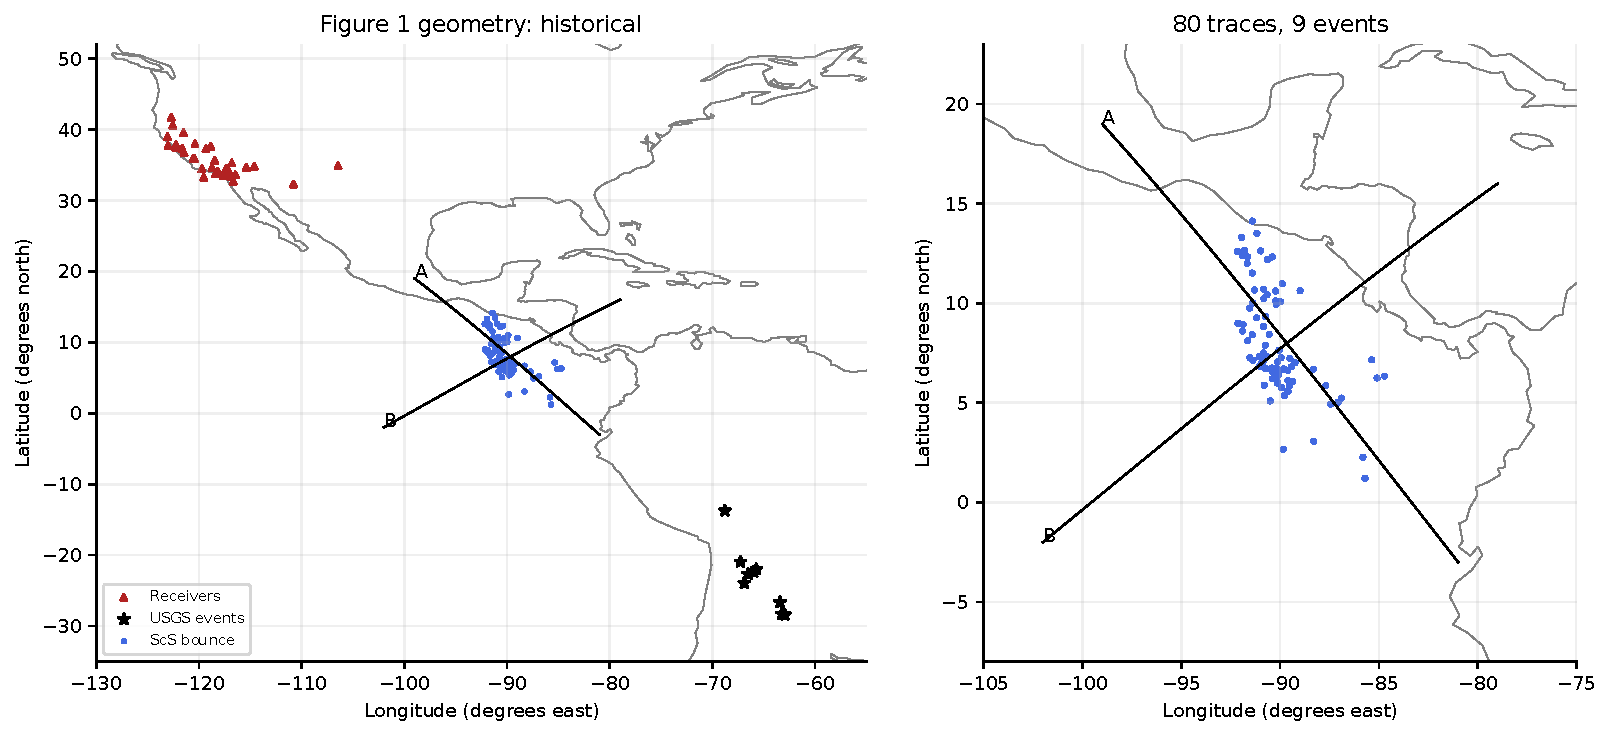
\includegraphics[width=.96\linewidth]{figures/historical/figure1.pdf}
\caption{historical; manuscript Figure 1 counterpart: Independently retrieved event and station geometry and calculated ScS bounce points. The two selected section directions are shown. Coastlines are Natural Earth geographic context.}\end{figure}
\begin{figure}[p]\centering
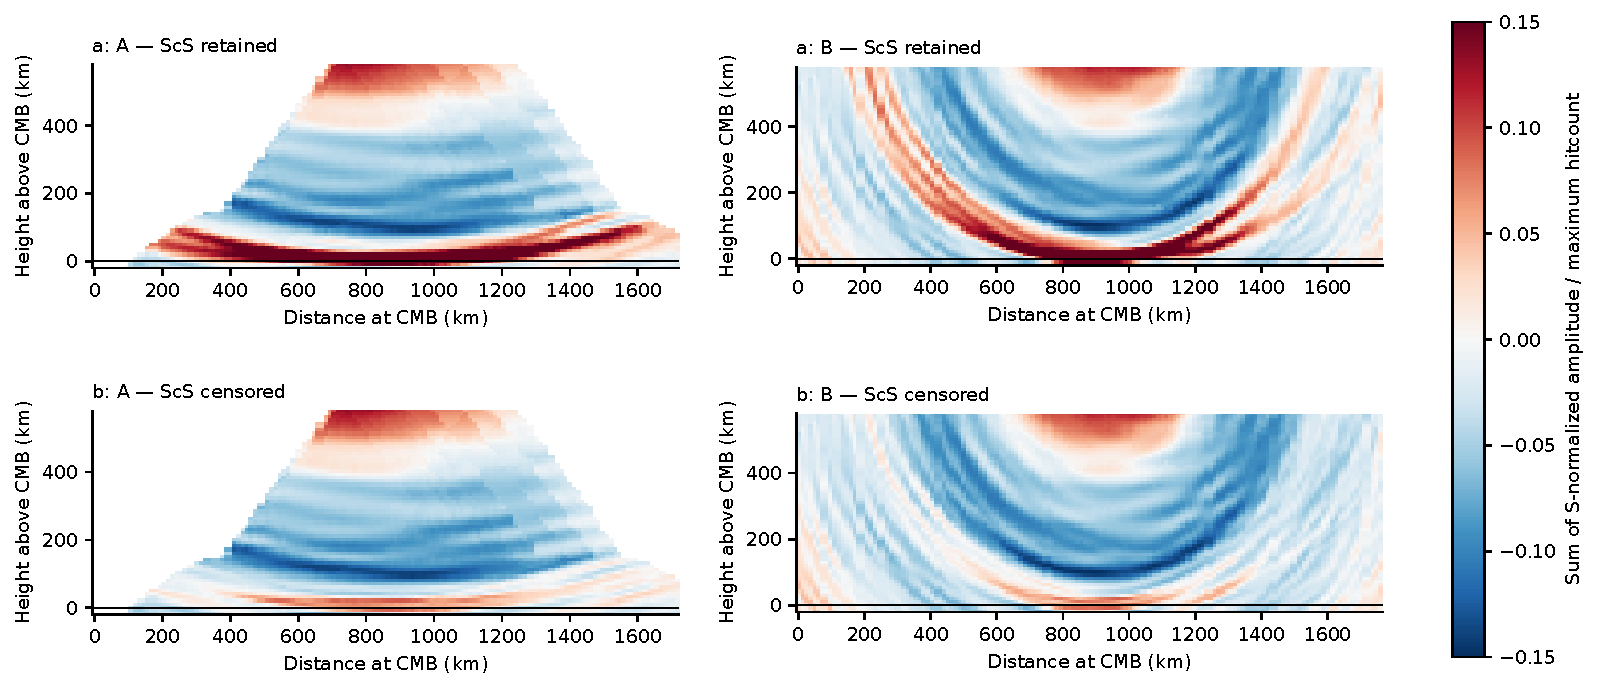
\includegraphics[width=.96\linewidth]{figures/historical/figure2.pdf}
\caption{historical; manuscript Figure 2 counterpart: Independent PREM migration. Top: ScS retained; bottom: ScS censored. Left: profile A; right: profile B. Both use ScS as reference and suppress S. Colour is the signed S-normalized stack weighted by relative hitcount, saturated at plus/minus 0.15. White regions fail the 20-trace/three-event display rule.}\end{figure}
\begin{figure}[p]\centering
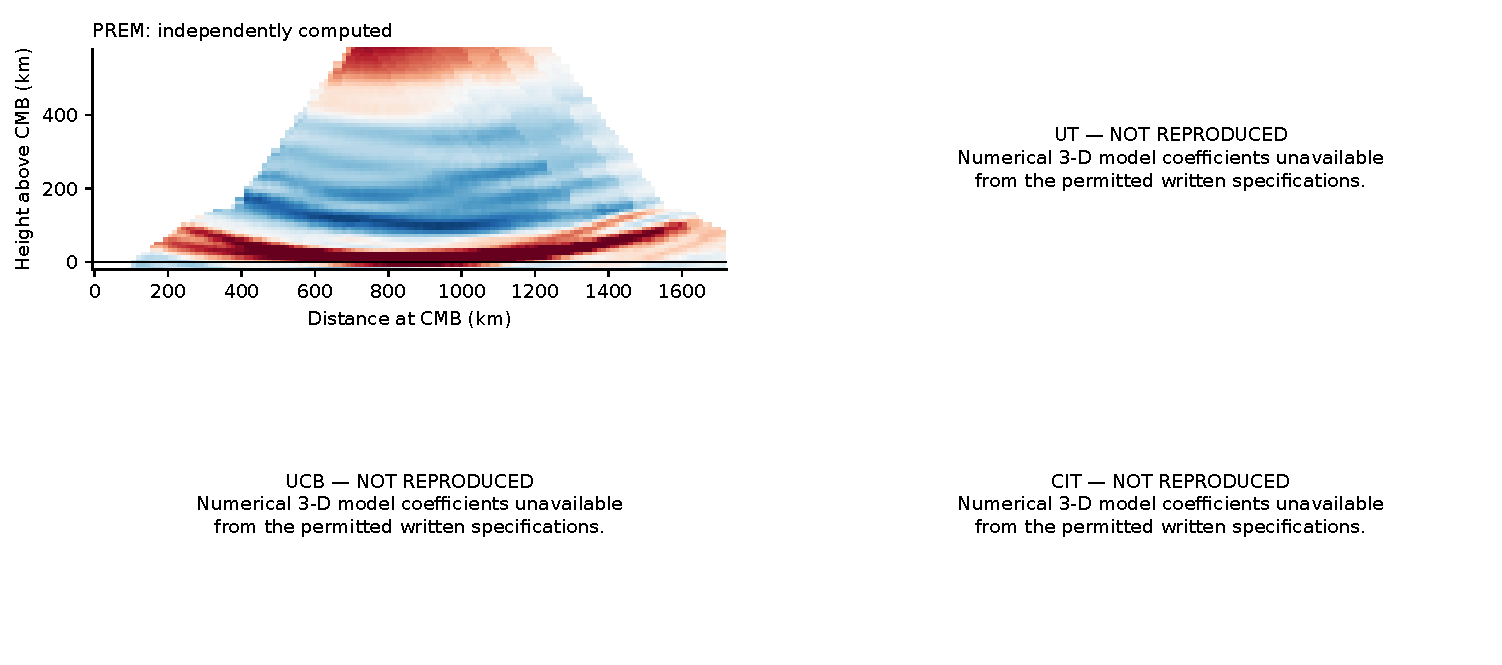
\includegraphics[width=.96\linewidth]{figures/historical/figure3.pdf}
\caption{historical; manuscript Figure 3 counterpart: Velocity-model comparison attempt. Only PREM is calculated. Blank, explicitly labelled UT, UCB and CIT panels identify unreproduced results; they are not filled with surrogate models.}\end{figure}
\begin{figure}[p]\centering
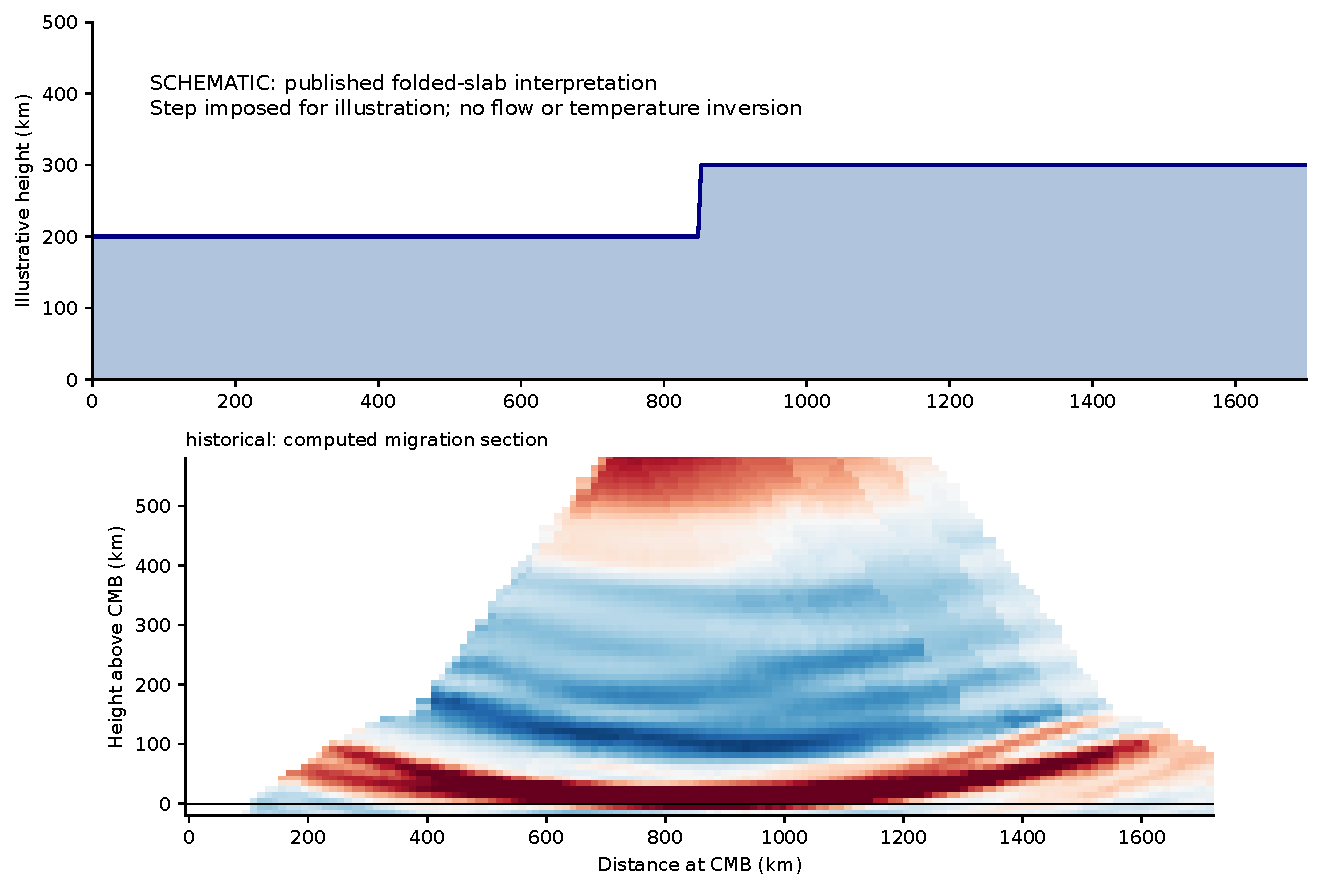
\includegraphics[width=.96\linewidth]{figures/historical/figure4.pdf}
\caption{historical; manuscript Figure 4 counterpart: Upper: an explicitly labelled conceptual schematic, with an imposed step and no calculated flow or temperature field. Lower: the independent observational profile A. The schematic is not evidence for a fold.}\end{figure}
\clearpage\subsection*{Set 3: modern\_same}
\begin{figure}[p]\centering
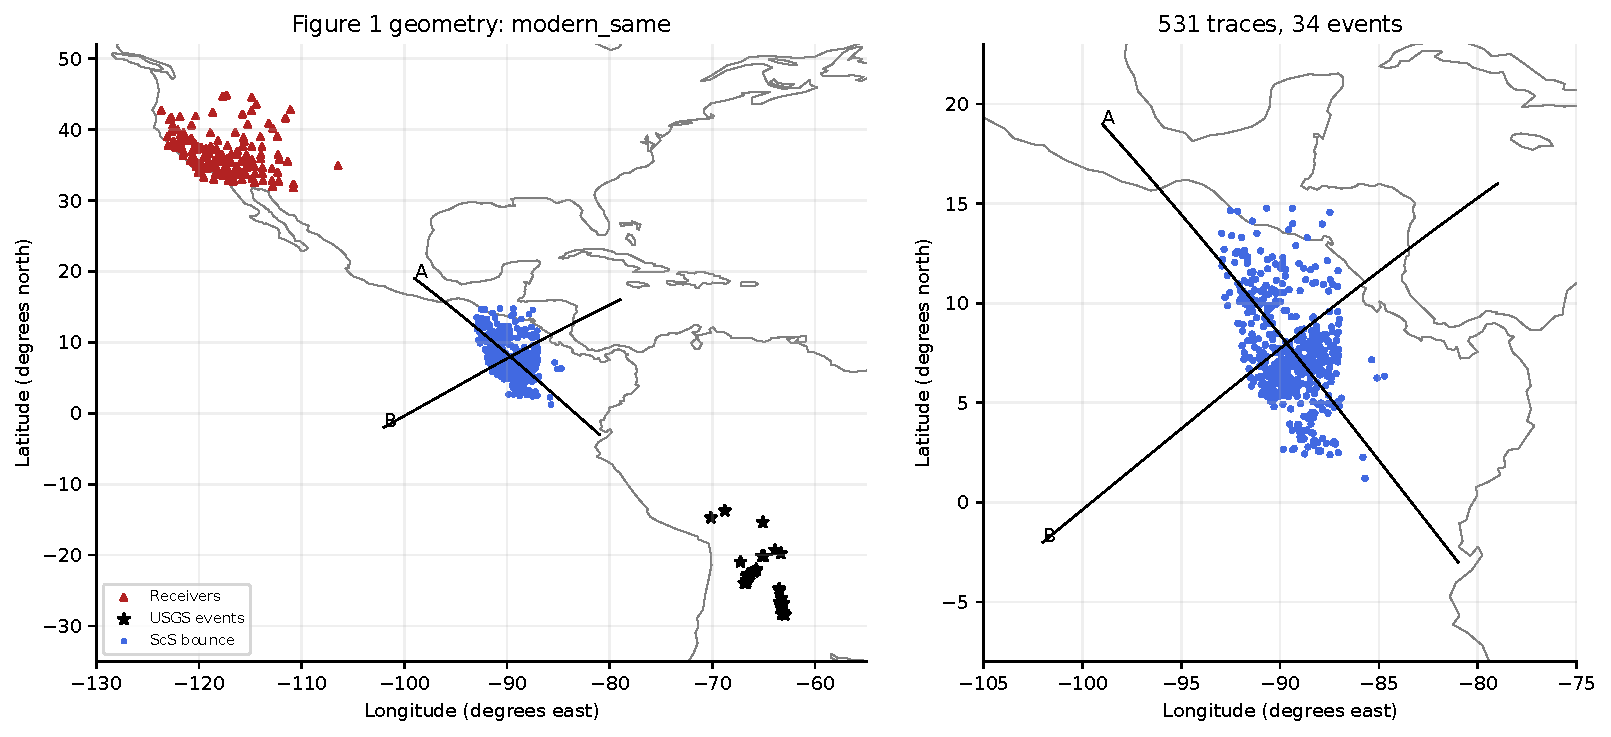
\includegraphics[width=.96\linewidth]{figures/modern_same/figure1.pdf}
\caption{modern\_same; manuscript Figure 1 counterpart: Independently retrieved event and station geometry and calculated ScS bounce points. The two selected section directions are shown. Coastlines are Natural Earth geographic context.}\end{figure}
\begin{figure}[p]\centering
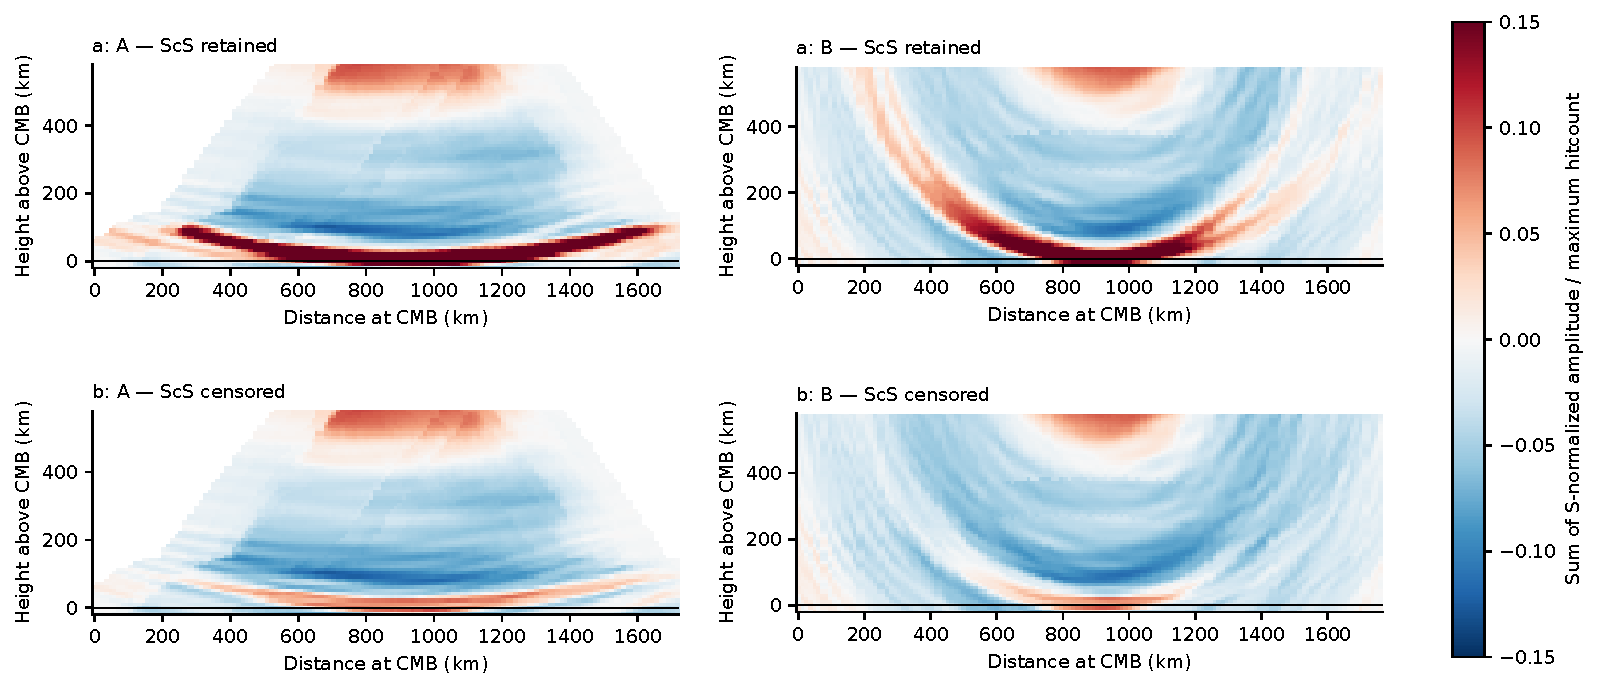
\includegraphics[width=.96\linewidth]{figures/modern_same/figure2.pdf}
\caption{modern\_same; manuscript Figure 2 counterpart: Independent PREM migration. Top: ScS retained; bottom: ScS censored. Left: profile A; right: profile B. Both use ScS as reference and suppress S. Colour is the signed S-normalized stack weighted by relative hitcount, saturated at plus/minus 0.15. White regions fail the 20-trace/three-event display rule.}\end{figure}
\begin{figure}[p]\centering
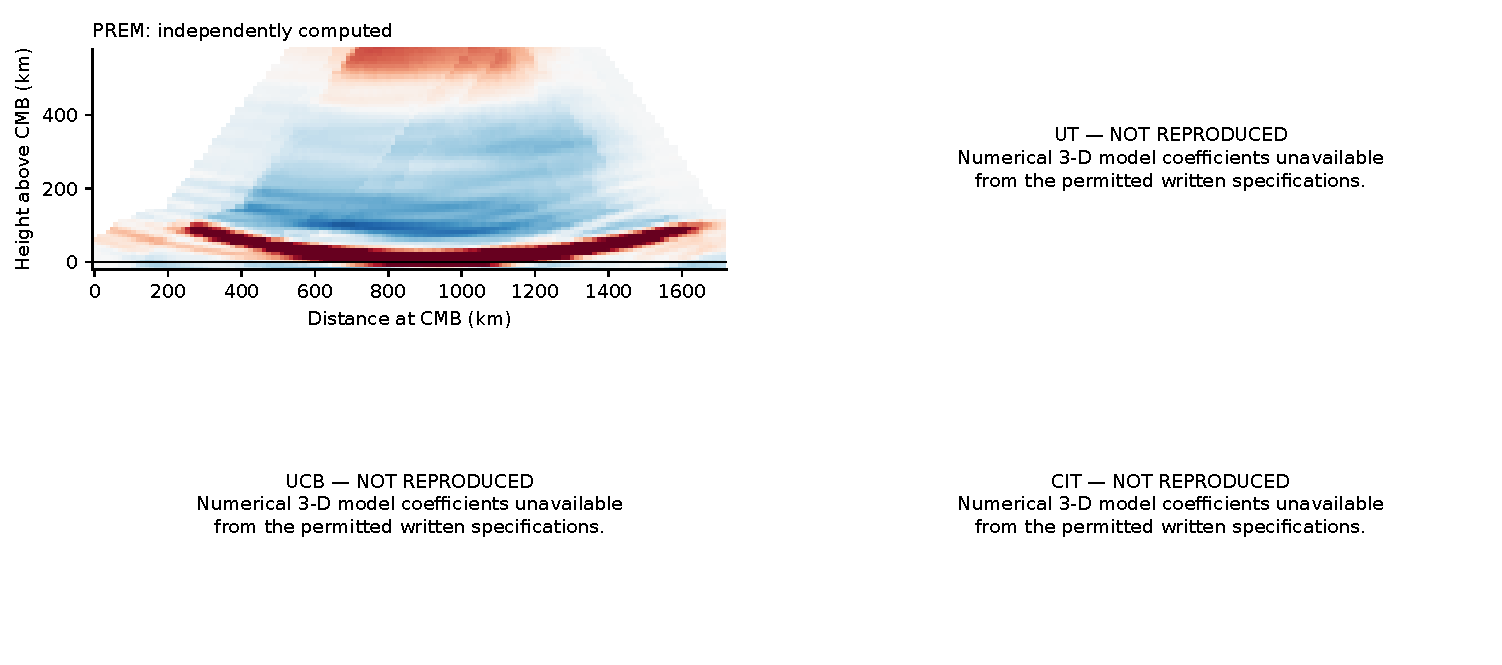
\includegraphics[width=.96\linewidth]{figures/modern_same/figure3.pdf}
\caption{modern\_same; manuscript Figure 3 counterpart: Velocity-model comparison attempt. Only PREM is calculated. Blank, explicitly labelled UT, UCB and CIT panels identify unreproduced results; they are not filled with surrogate models.}\end{figure}
\begin{figure}[p]\centering
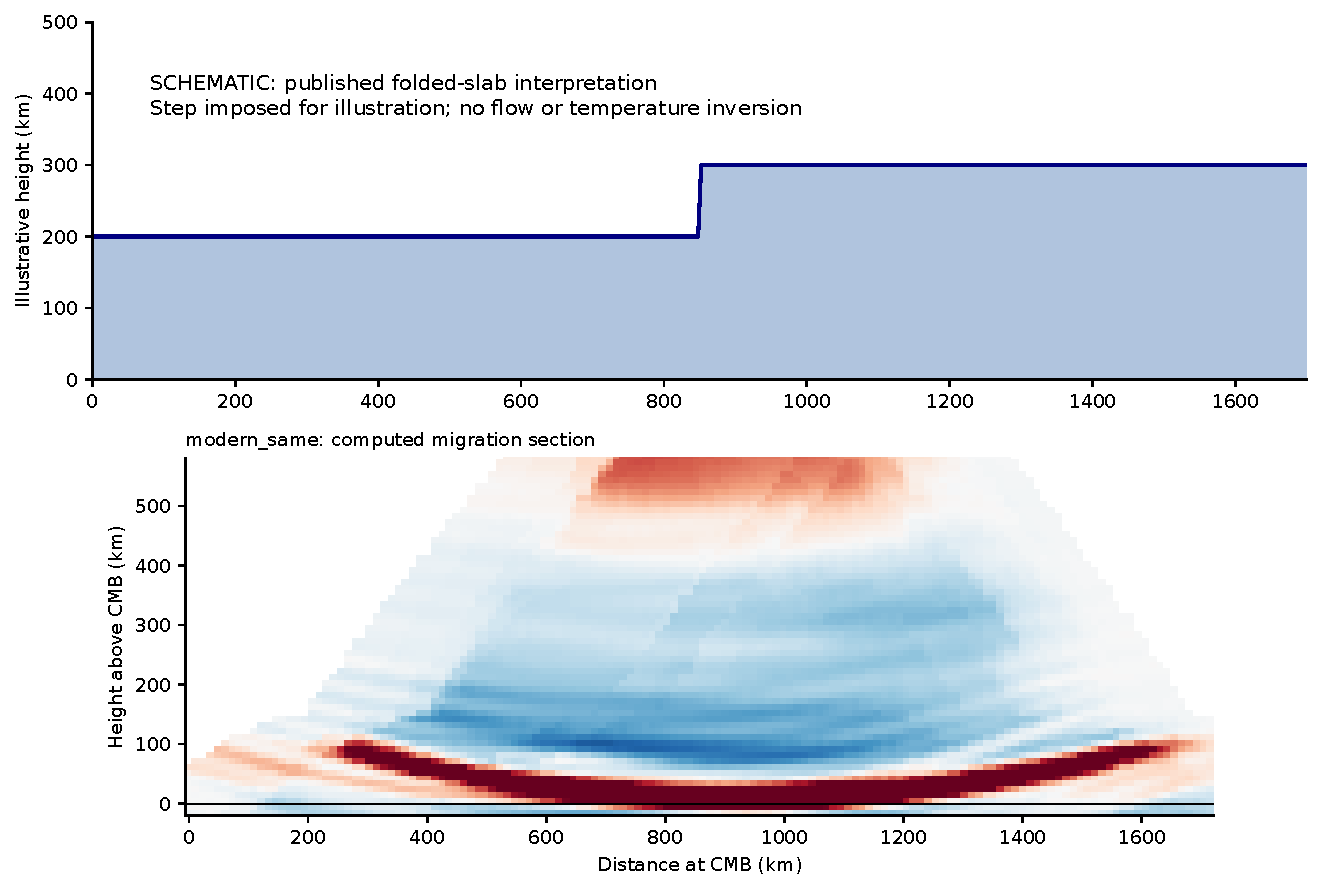
\includegraphics[width=.96\linewidth]{figures/modern_same/figure4.pdf}
\caption{modern\_same; manuscript Figure 4 counterpart: Upper: an explicitly labelled conceptual schematic, with an imposed step and no calculated flow or temperature field. Lower: the independent observational profile A. The schematic is not evidence for a fold.}\end{figure}
\clearpage\subsection*{Set 4: expanded}
The wider calculation covers 10 degrees S--25 degrees N and 110--70 degrees W. Profiles A and B are retained for direct comparison; the horizontal slices in supplementary Figure 5 show the additional imaged region, with the same coverage threshold.
\begin{figure}[p]\centering
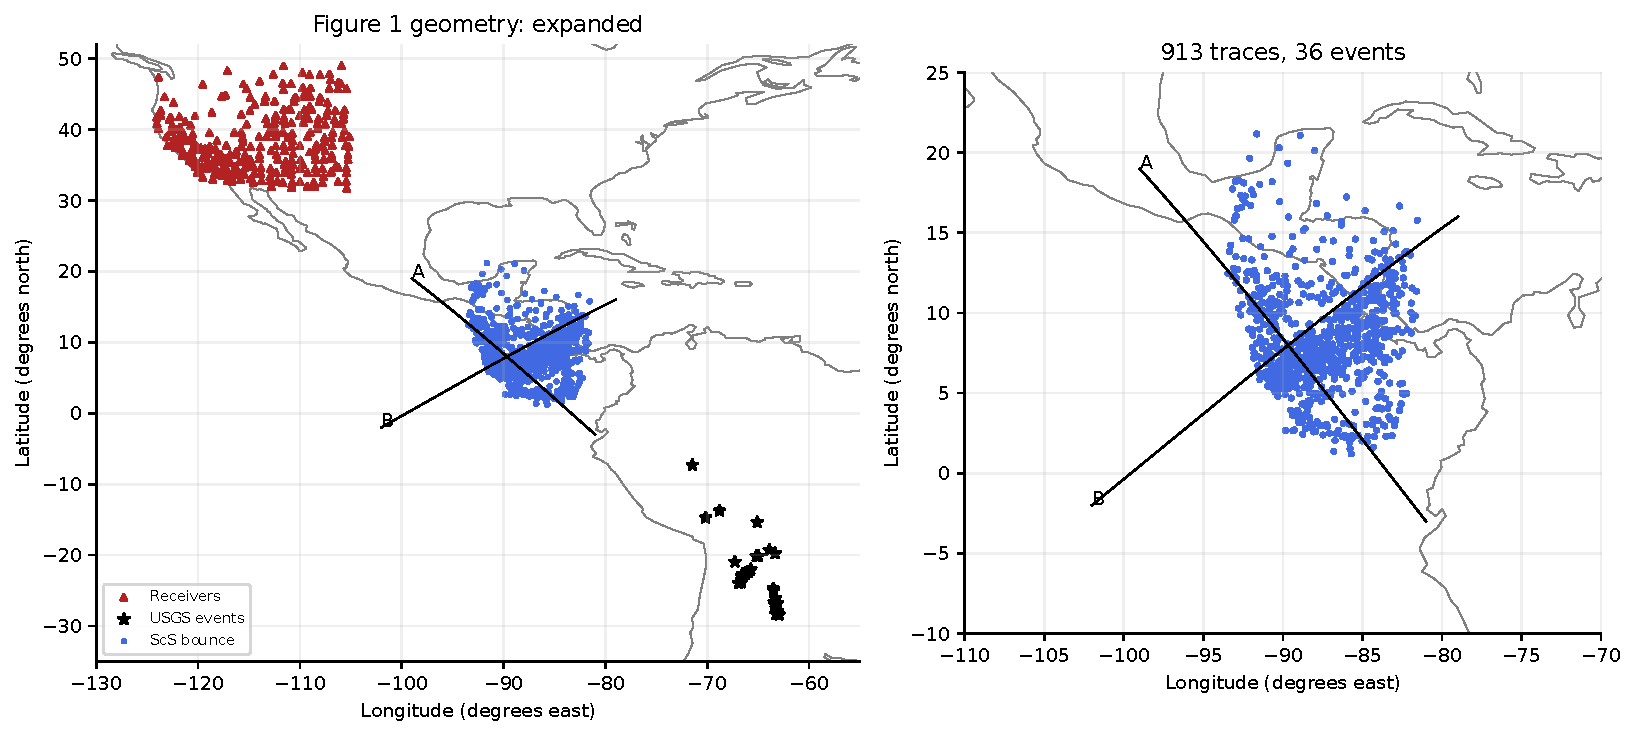
\includegraphics[width=.96\linewidth]{figures/expanded/figure1.pdf}
\caption{expanded; manuscript Figure 1 counterpart: Independently retrieved event and station geometry and calculated ScS bounce points. The two selected section directions are shown. Coastlines are Natural Earth geographic context.}\end{figure}
\begin{figure}[p]\centering
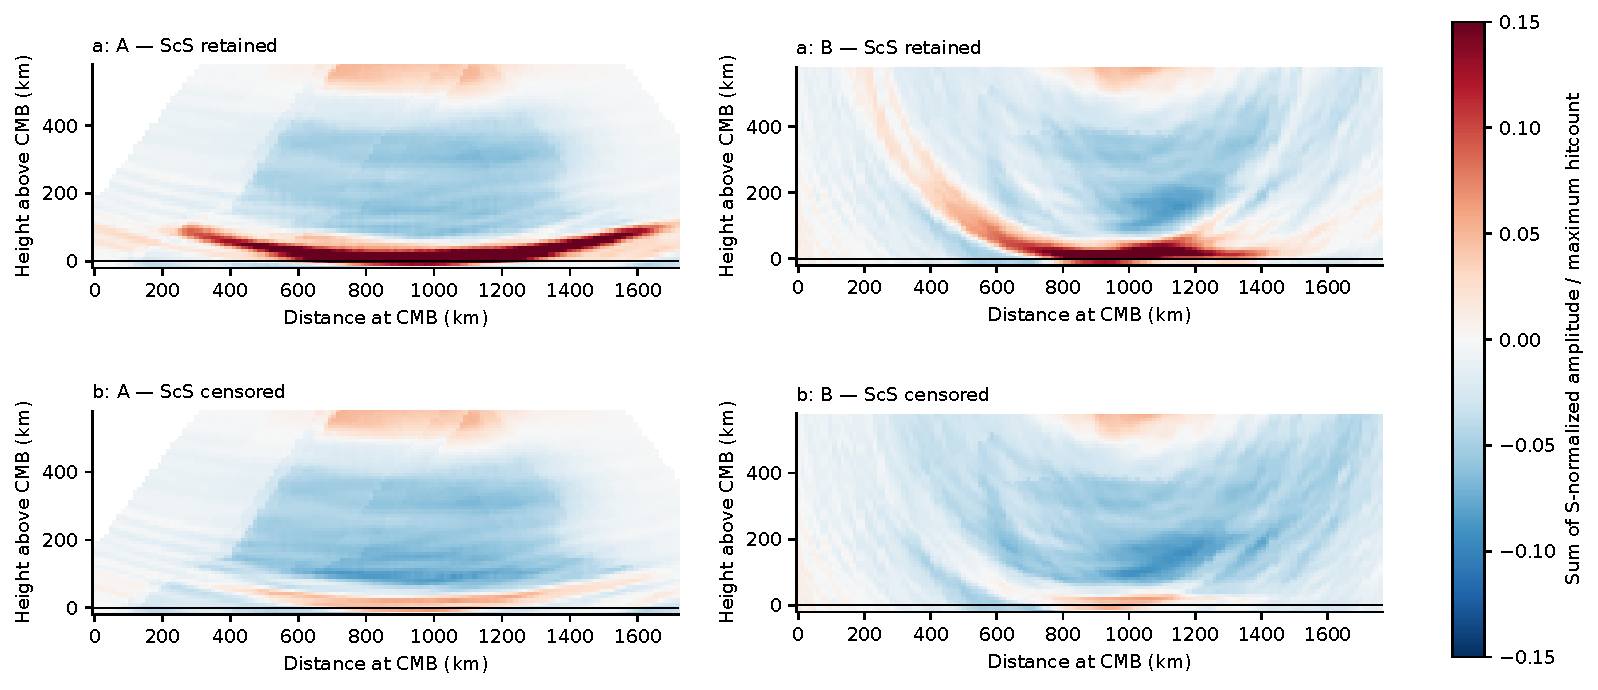
\includegraphics[width=.96\linewidth]{figures/expanded/figure2.pdf}
\caption{expanded; manuscript Figure 2 counterpart: Independent PREM migration. Top: ScS retained; bottom: ScS censored. Left: profile A; right: profile B. Both use ScS as reference and suppress S. Colour is the signed S-normalized stack weighted by relative hitcount, saturated at plus/minus 0.15. White regions fail the 20-trace/three-event display rule.}\end{figure}
\begin{figure}[p]\centering
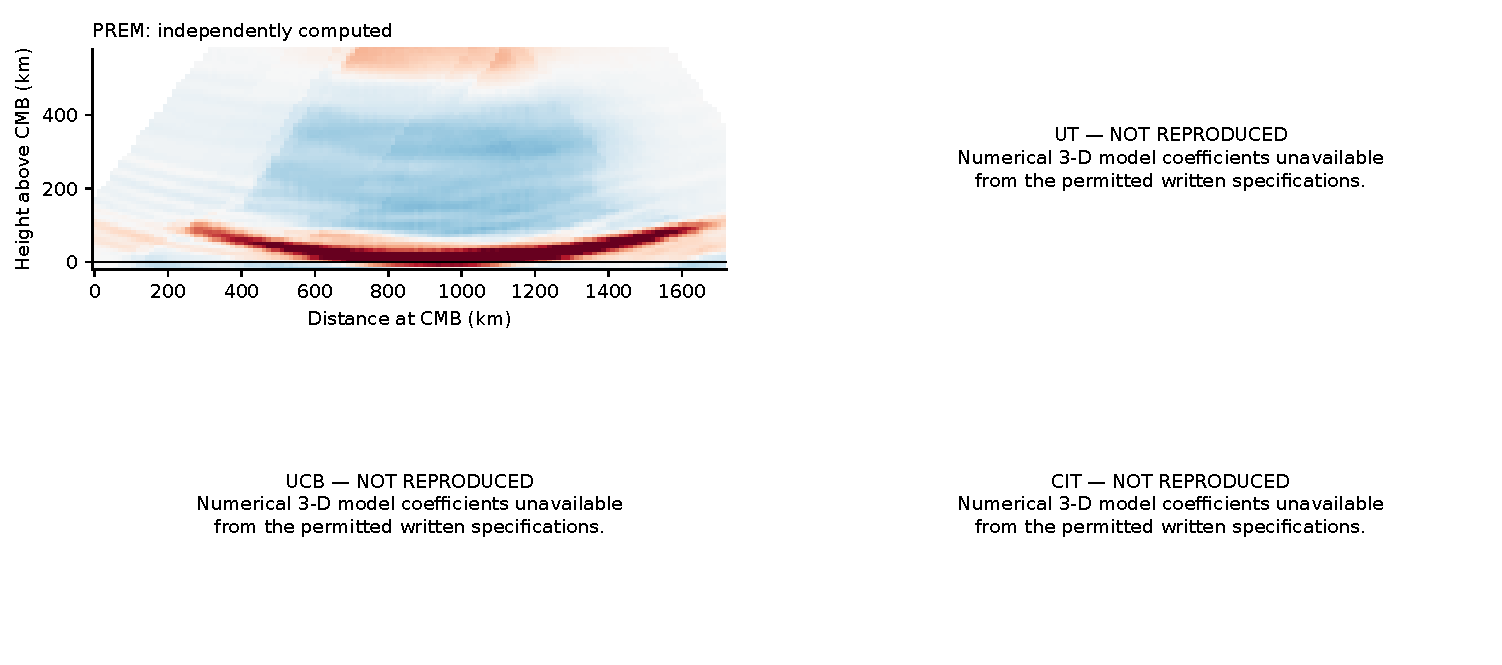
\includegraphics[width=.96\linewidth]{figures/expanded/figure3.pdf}
\caption{expanded; manuscript Figure 3 counterpart: Velocity-model comparison attempt. Only PREM is calculated. Blank, explicitly labelled UT, UCB and CIT panels identify unreproduced results; they are not filled with surrogate models.}\end{figure}
\begin{figure}[p]\centering
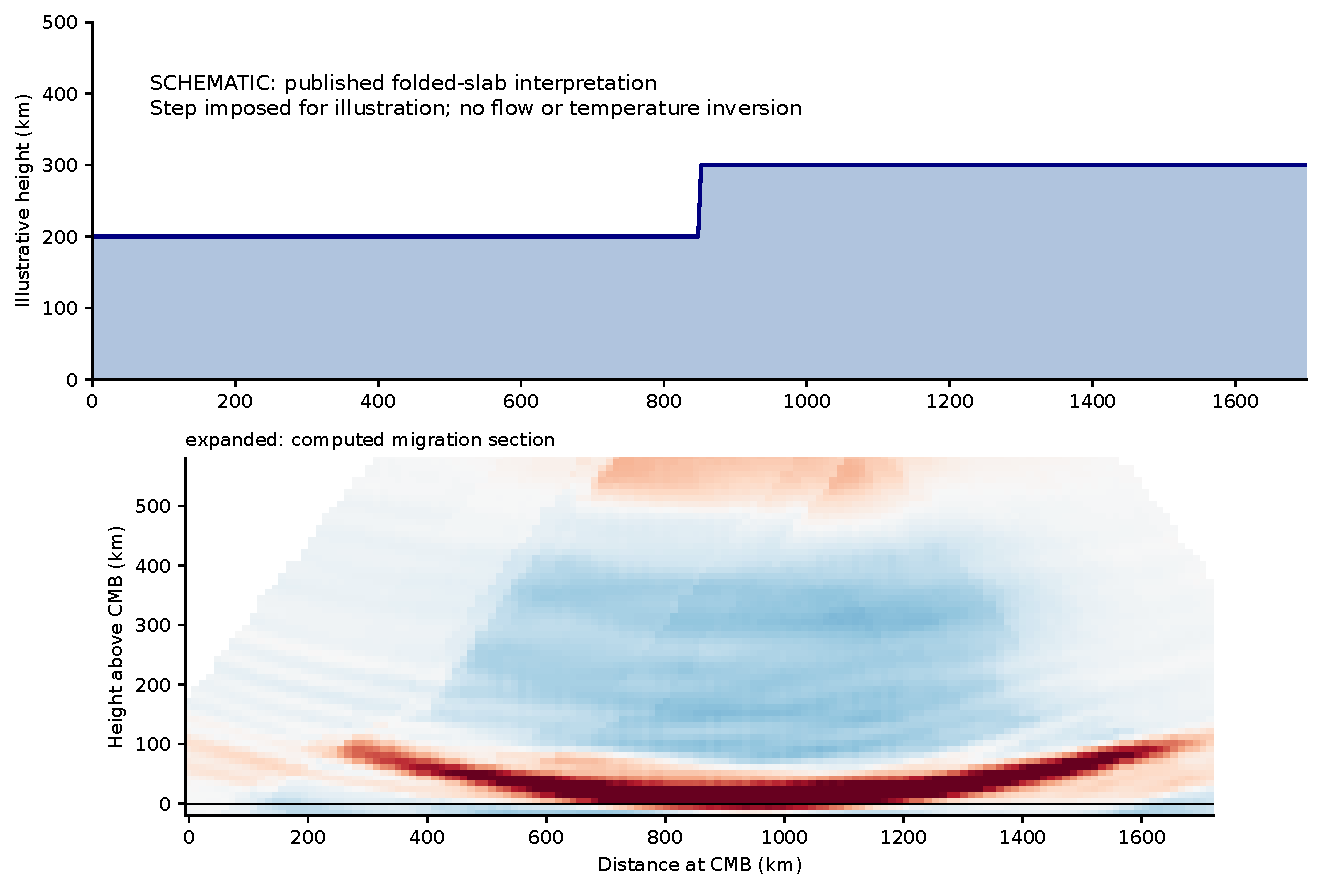
\includegraphics[width=.96\linewidth]{figures/expanded/figure4.pdf}
\caption{expanded; manuscript Figure 4 counterpart: Upper: an explicitly labelled conceptual schematic, with an imposed step and no calculated flow or temperature field. Lower: the independent observational profile A. The schematic is not evidence for a fold.}\end{figure}
\clearpage\section{Supplementary calculations}
\begin{figure}[p]\centering
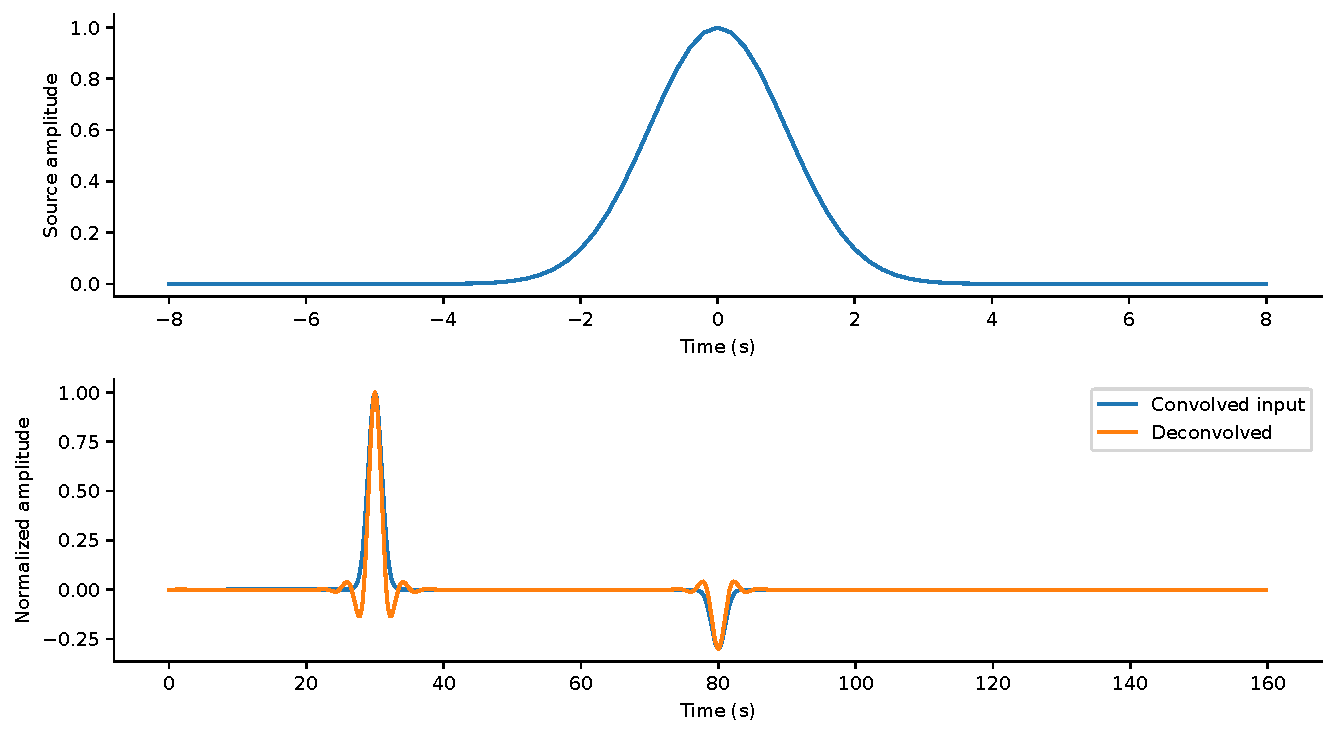
\includegraphics[width=.96\linewidth]{figures/validation.pdf}
\caption{Synthetic deconvolution consistency test. The input consists of two known signed impulses convolved with the displayed wavelet. This is a validation signal, not Earth data.}\end{figure}
\begin{figure}[p]\centering
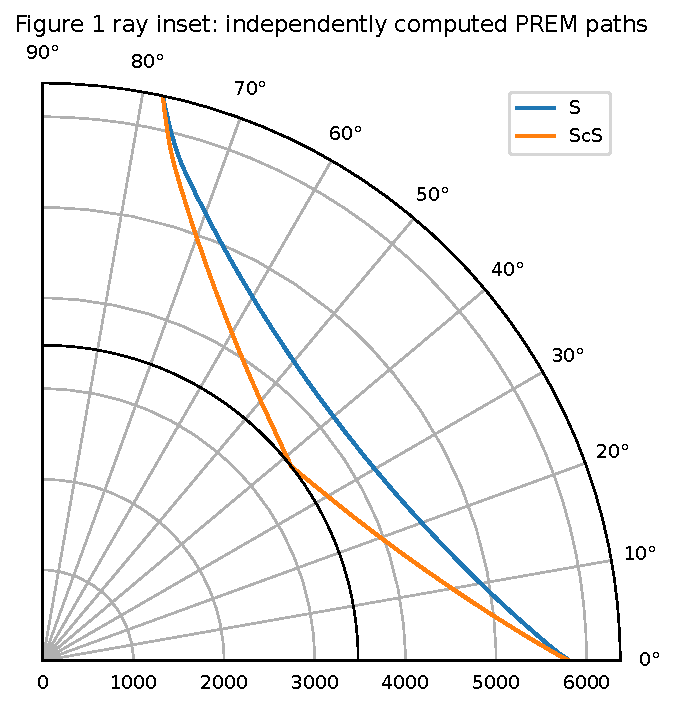
\includegraphics[width=.96\linewidth]{figures/figure1-rays.pdf}
\caption{Independently calculated S and ScS paths for a 558 km source at 78 degrees. This is a numerical ray diagram; the publication does not specify the exact illustrative source used in its inset.}\end{figure}
\begin{figure}[p]\centering
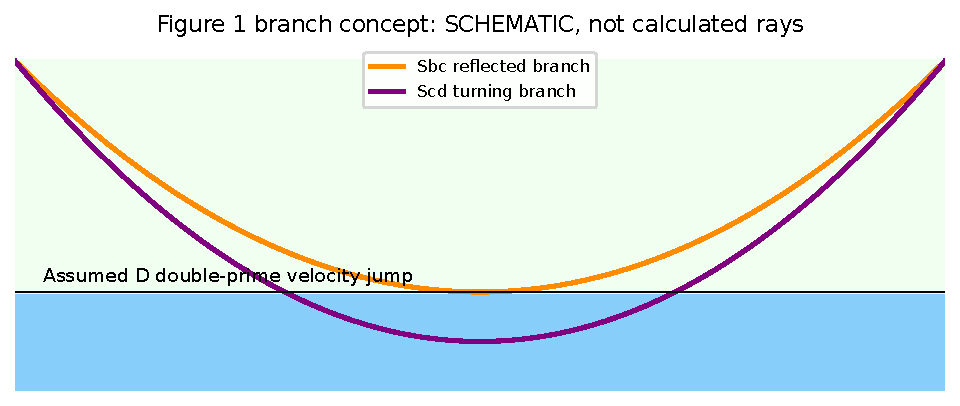
\includegraphics[width=.96\linewidth]{figures/figure1-triplication-schematic.pdf}
\caption{Redrawn conceptual companion to the Figure 1 triplication inset. The curves only distinguish reflection above the jump from turning below it. They do not satisfy a calculated ray equation and are not reproduced numerical results.}\end{figure}
\begin{figure}[p]\centering
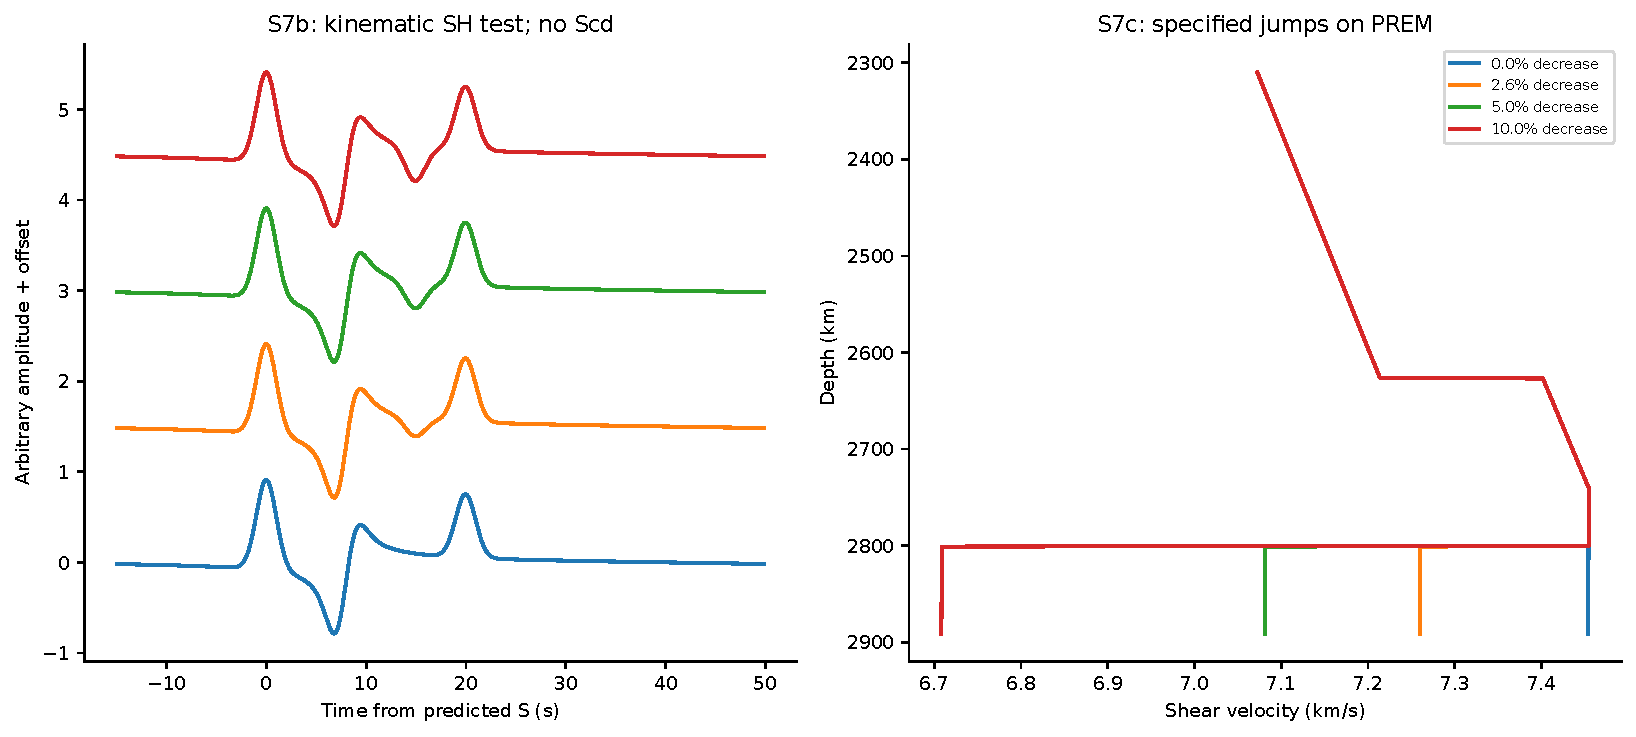
\includegraphics[width=.96\linewidth]{figures/supplement7bc.pdf}
\caption{Partial attempt at supplementary Figure 7b,c: local SH reflection coefficients and explicitly assumed layered velocity profiles. There is no refracted Scd branch or full-wave reflectivity calculation; these curves cannot reproduce the published triplication amplitudes.}\end{figure}
\begin{figure}[p]\centering
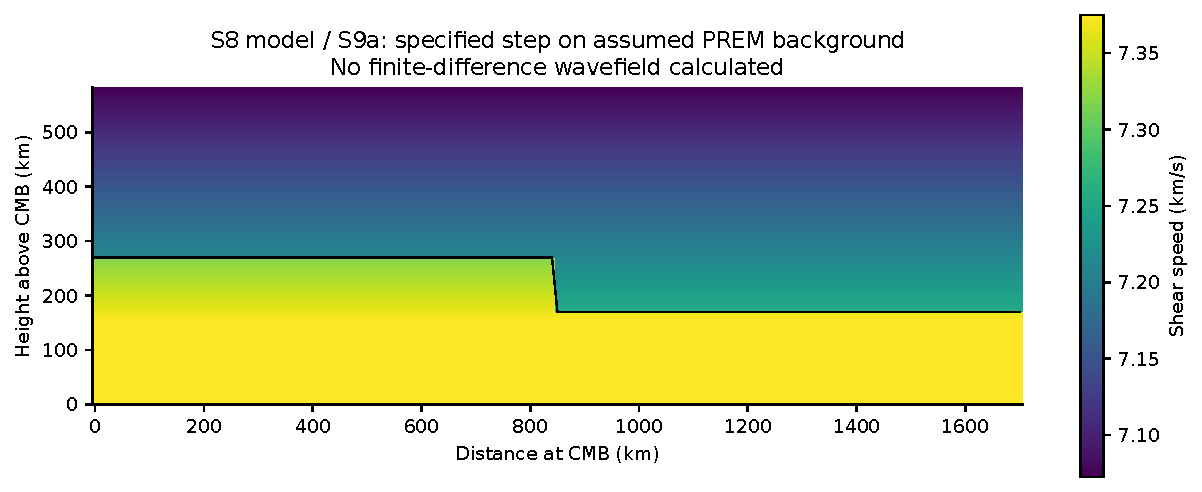
\includegraphics[width=.96\linewidth]{figures/step-model.pdf}
\caption{Numerical input-model illustration for supplementary Figures 8 and 9a. The stated 170/270 km heights and 1.5 percent jump are imposed on PREM. No full-wave propagation has been performed.}\end{figure}
\begin{figure}[p]\centering
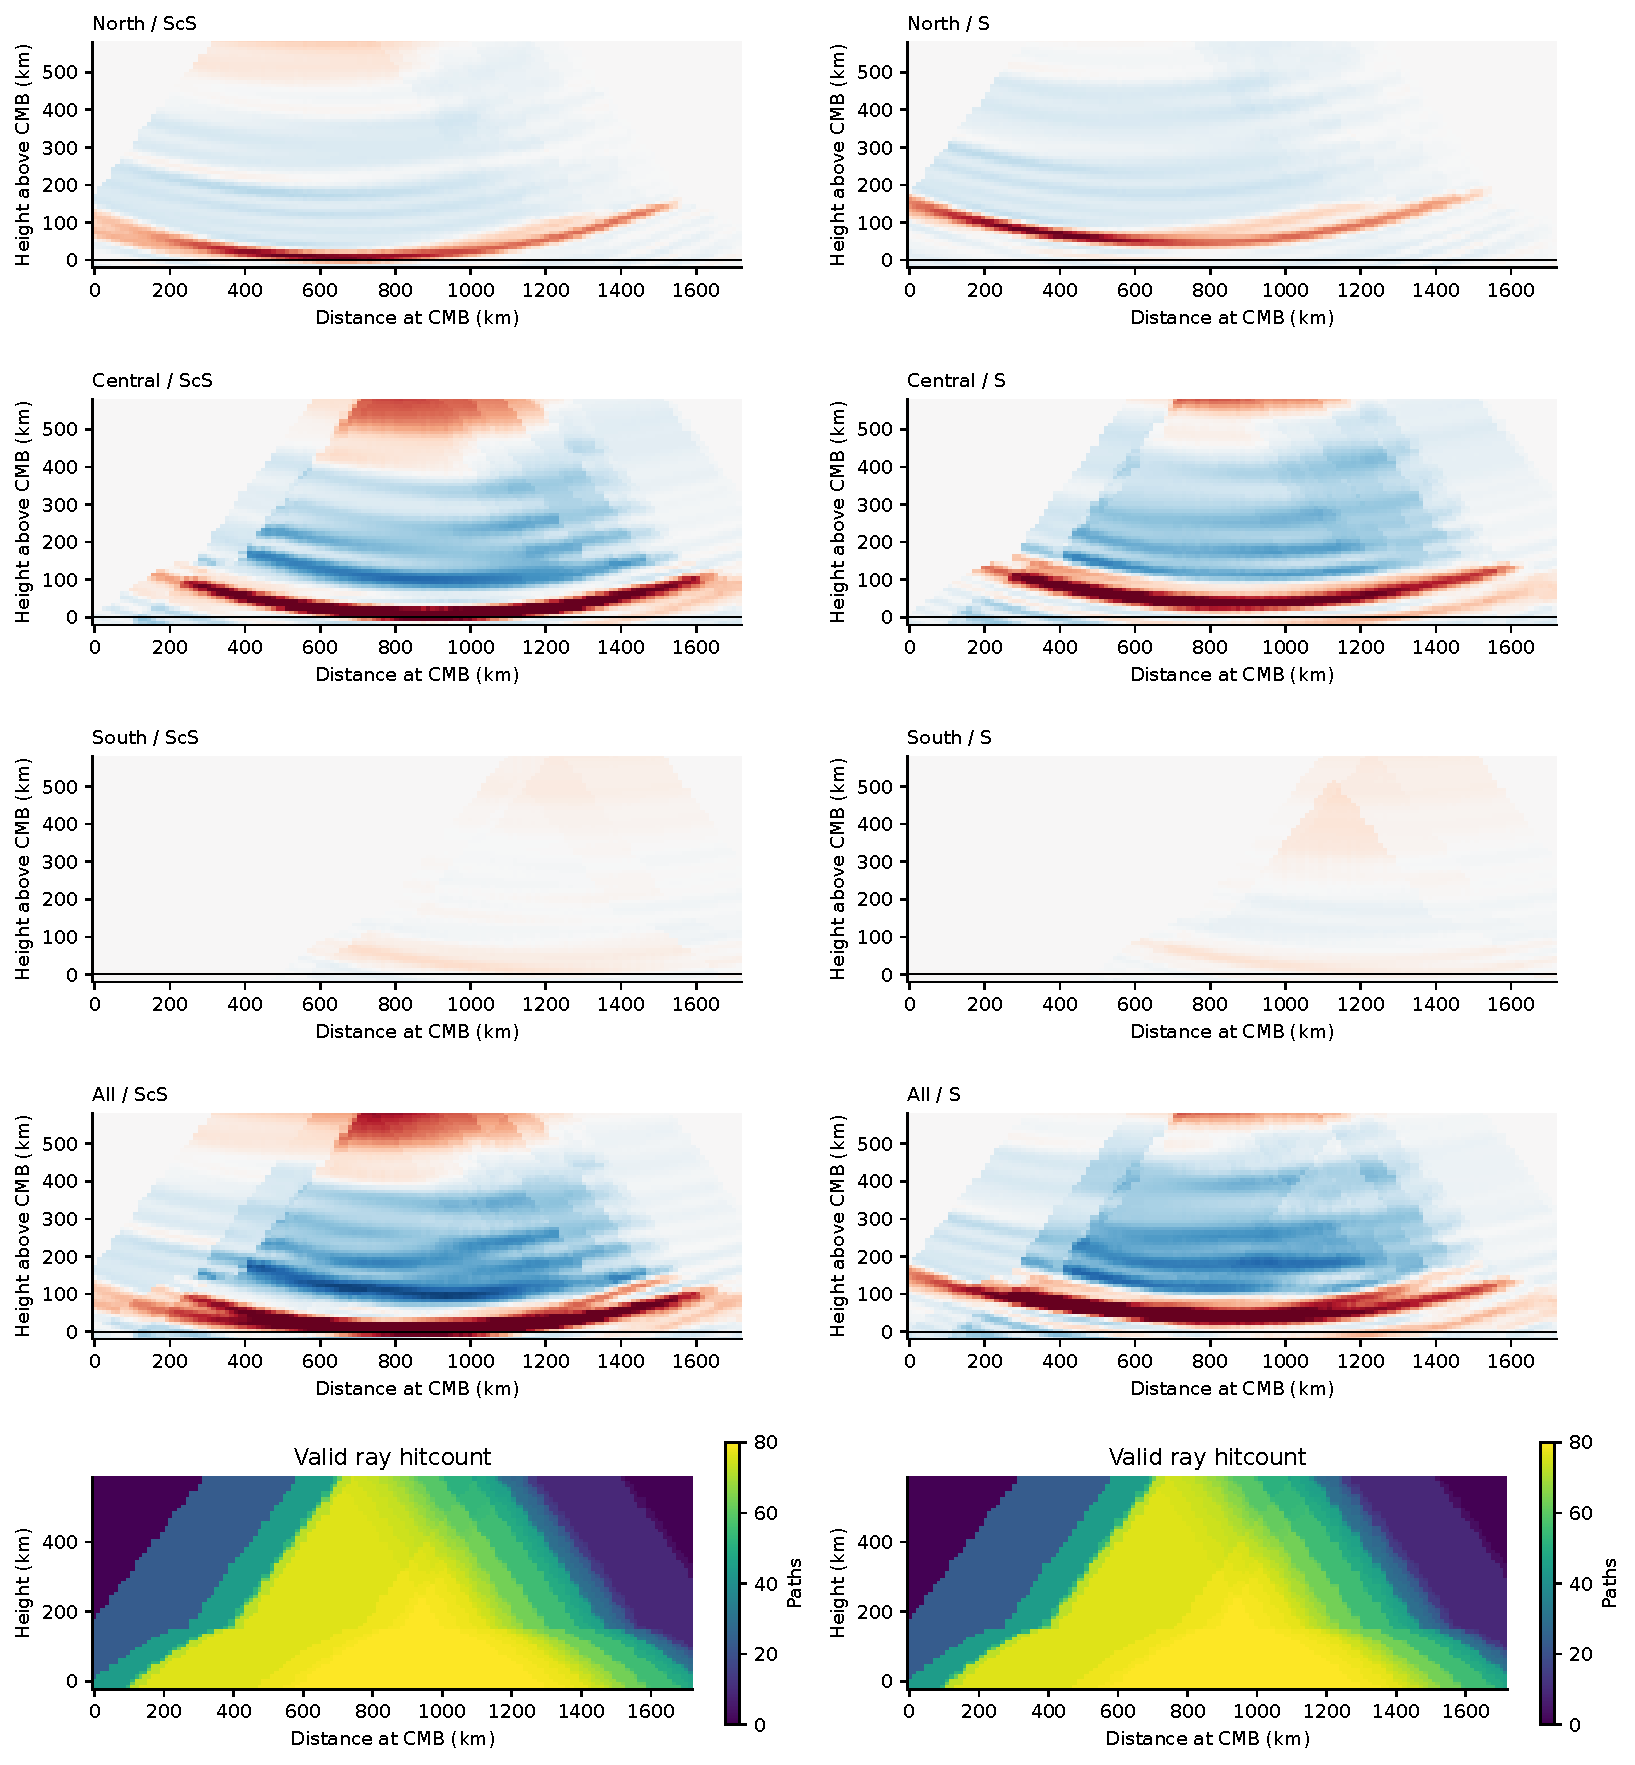
\includegraphics[width=.96\linewidth,height=.87\textheight,keepaspectratio]{figures/historical/supplement2.pdf}
\caption{historical; independent supplementary figure 2 counterpart. Definitions, assumptions, and panel status are given in the panel record. All numerical values come from saved arrays.}\end{figure}
\begin{figure}[p]\centering
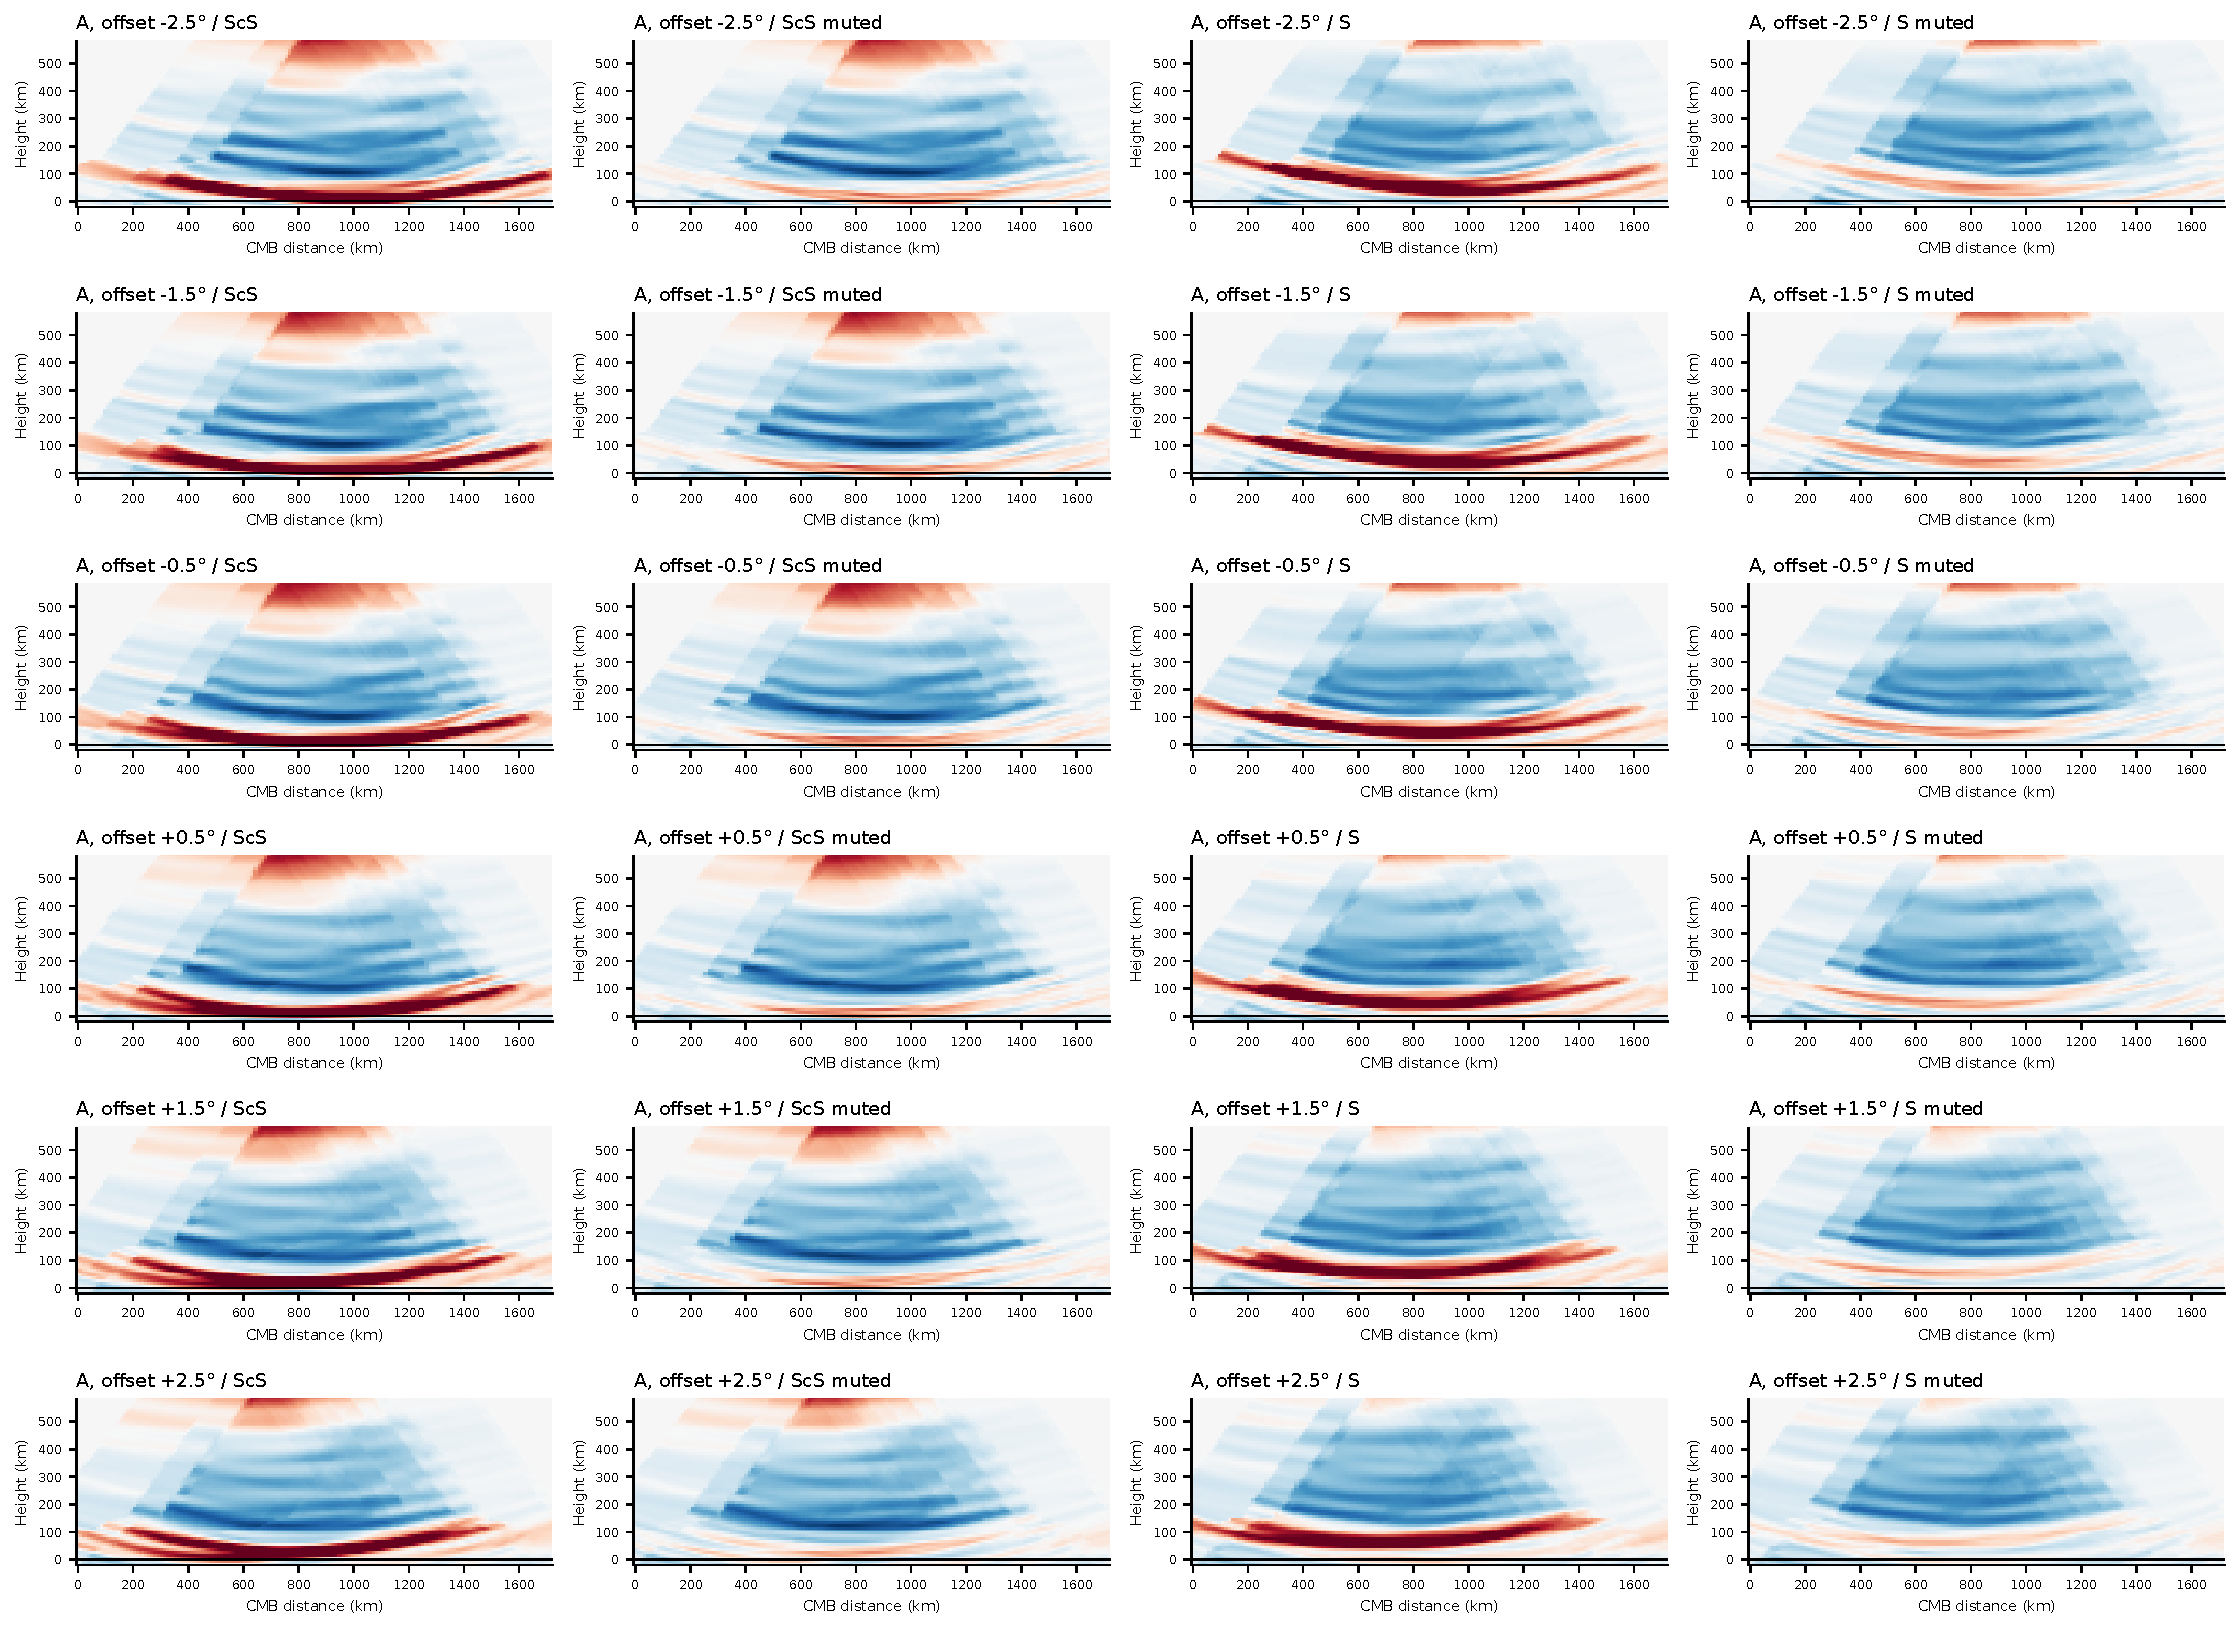
\includegraphics[width=.96\linewidth,height=.87\textheight,keepaspectratio]{figures/historical/supplement3a.pdf}
\caption{historical; independent supplementary figure 3a counterpart. Definitions, assumptions, and panel status are given in the panel record. All numerical values come from saved arrays.}\end{figure}
\begin{figure}[p]\centering
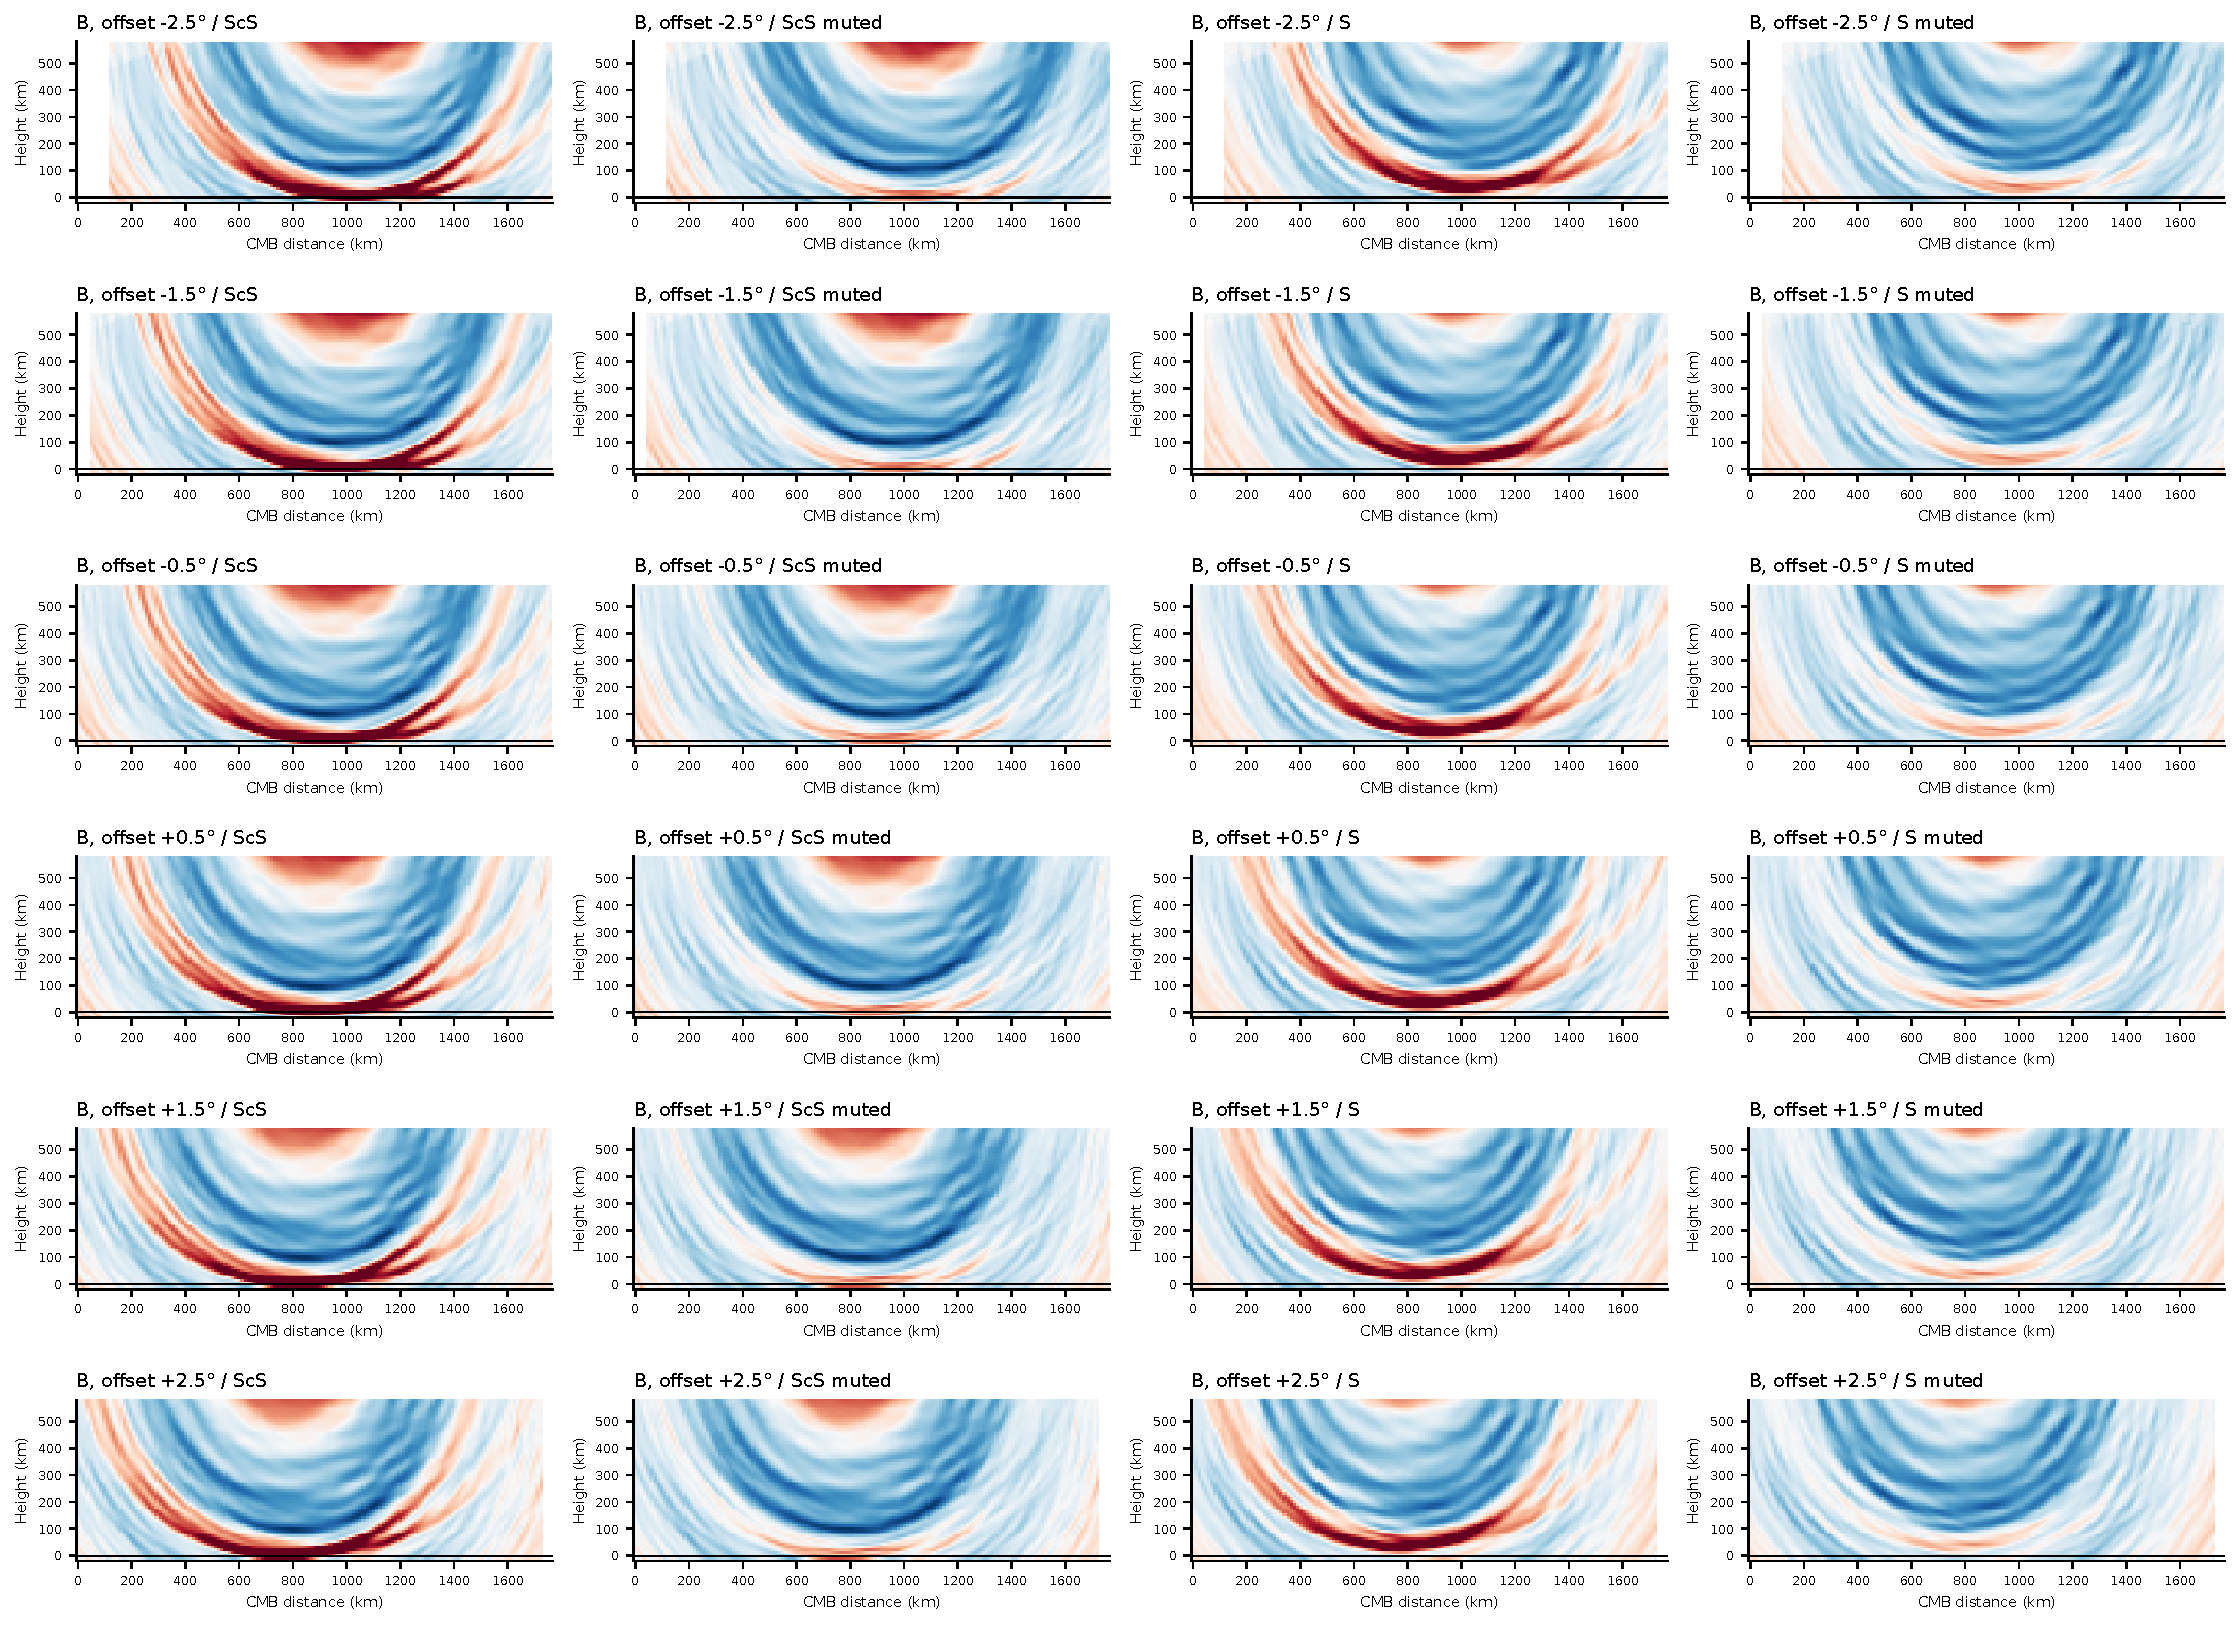
\includegraphics[width=.96\linewidth,height=.87\textheight,keepaspectratio]{figures/historical/supplement3b.pdf}
\caption{historical; independent supplementary figure 3b counterpart. Definitions, assumptions, and panel status are given in the panel record. All numerical values come from saved arrays.}\end{figure}
\begin{figure}[p]\centering
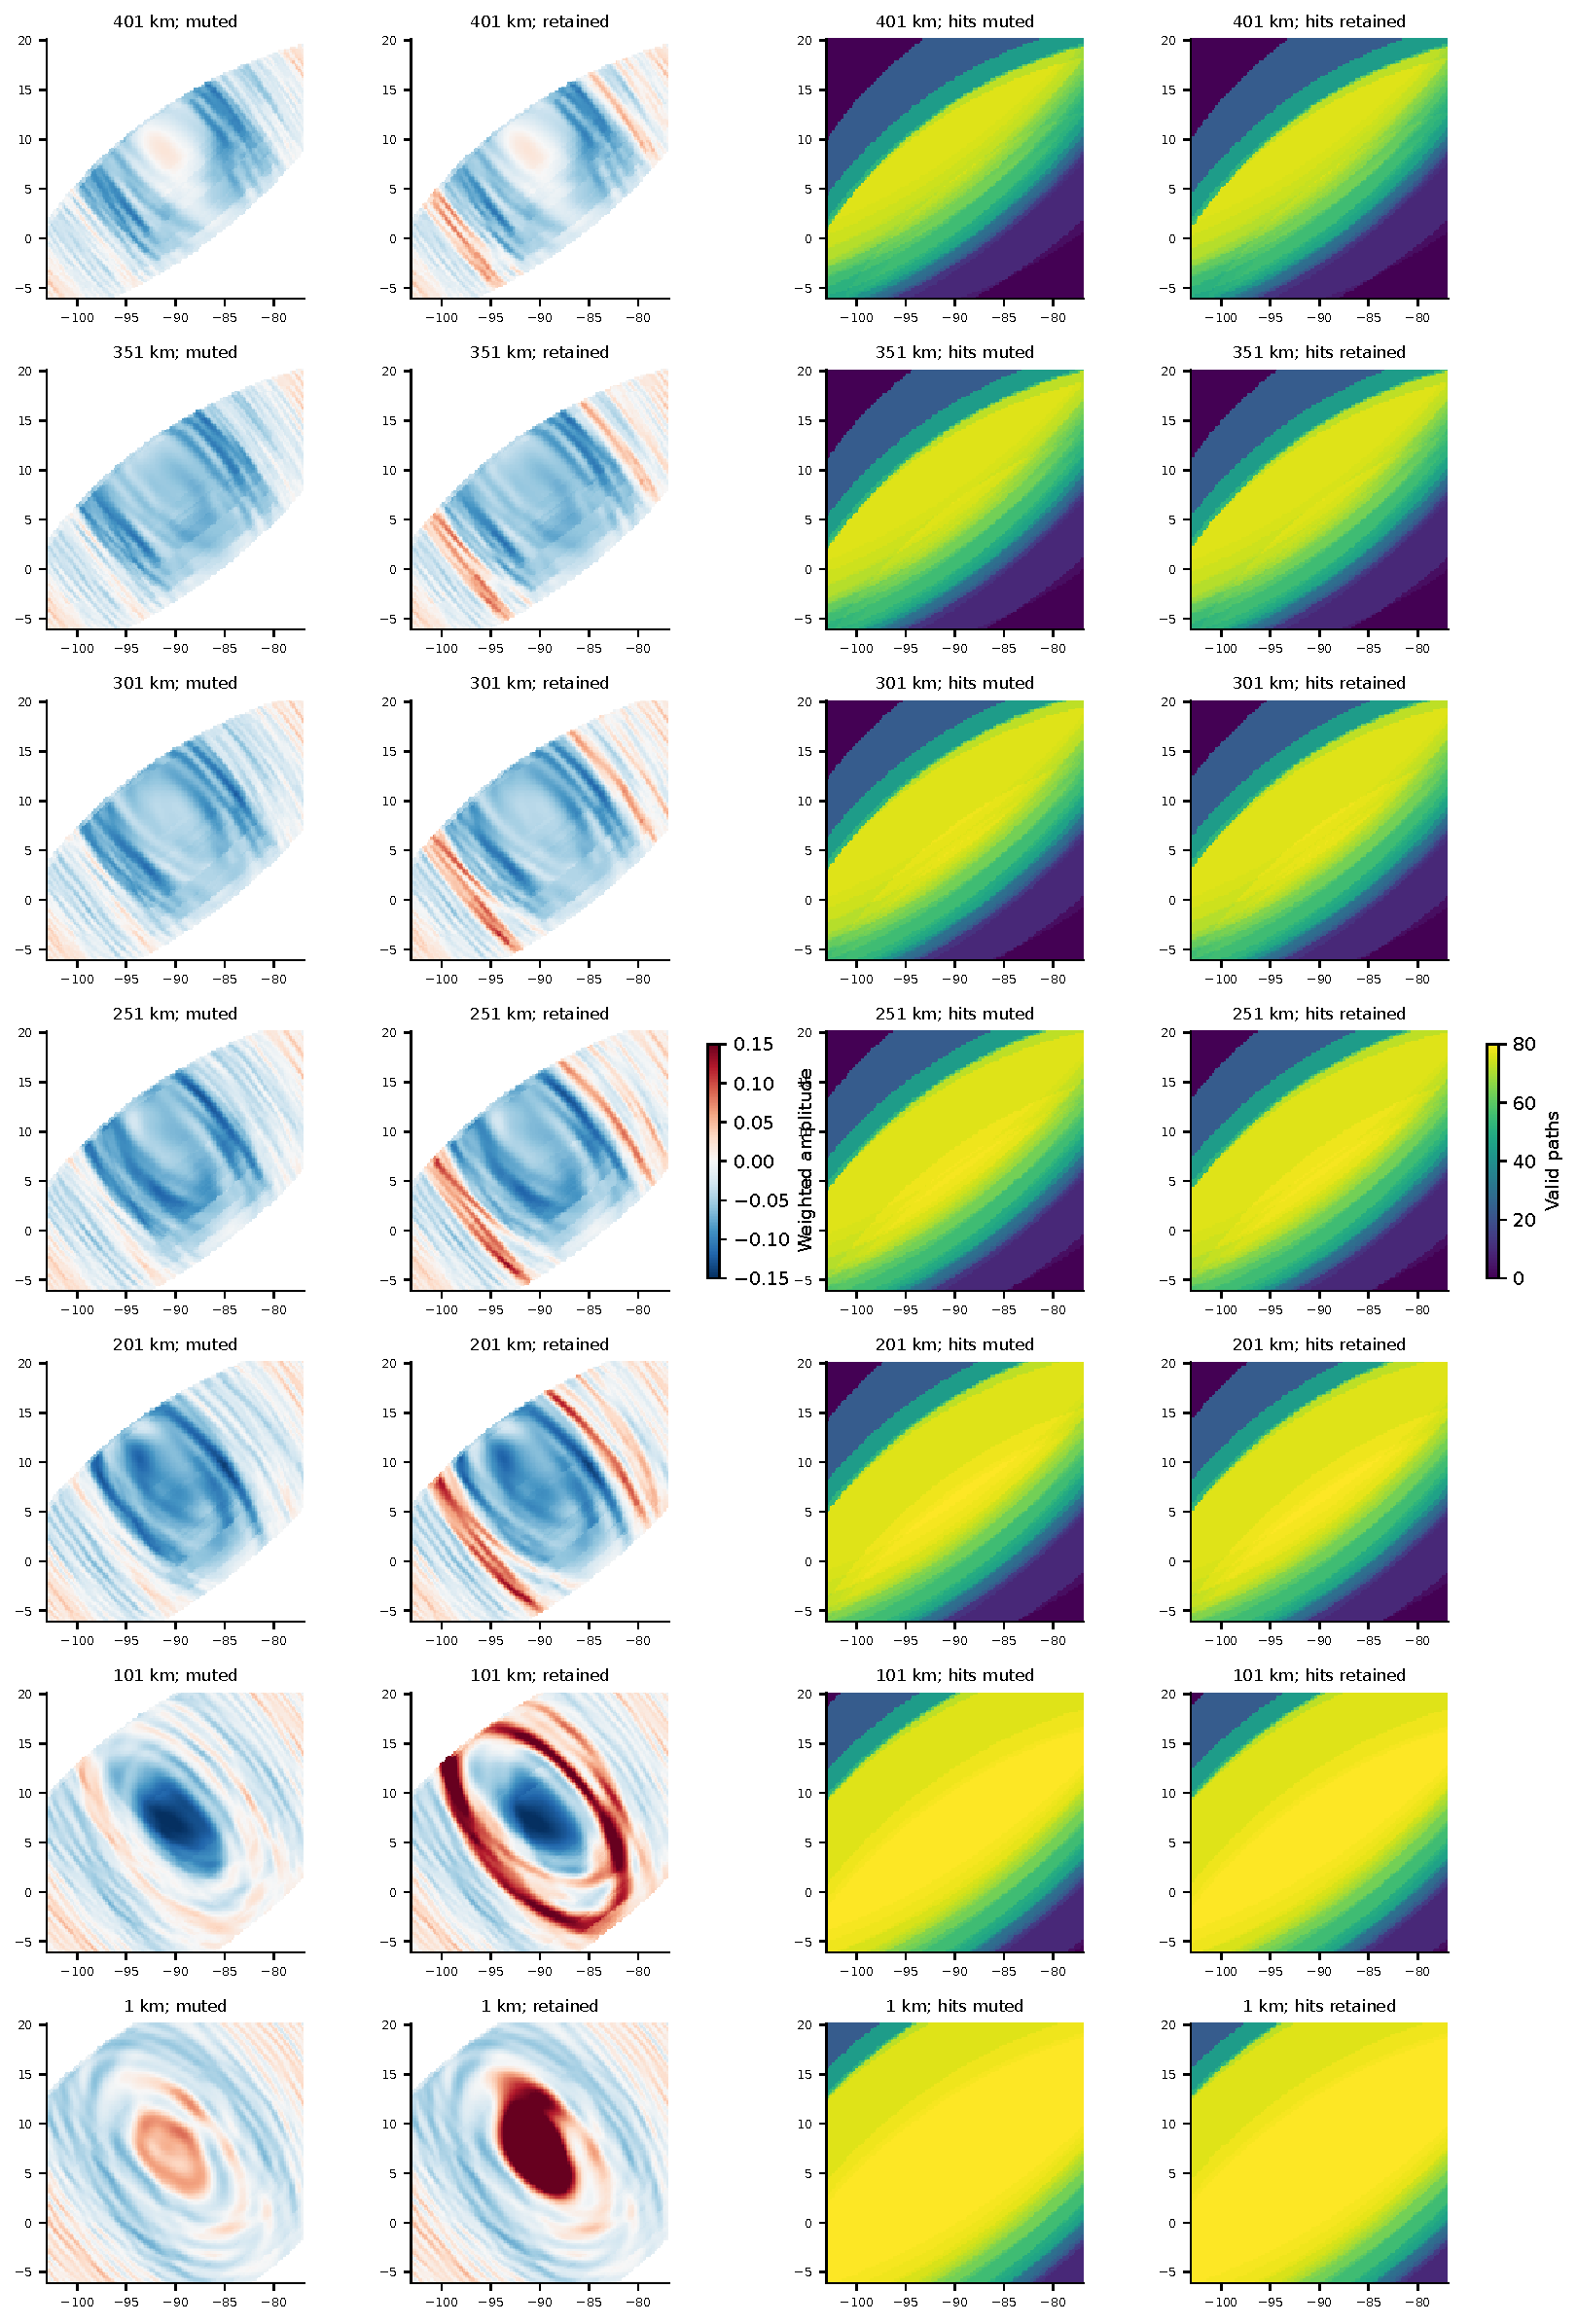
\includegraphics[width=.96\linewidth,height=.87\textheight,keepaspectratio]{figures/historical/supplement5.pdf}
\caption{historical; independent supplementary figure 5 counterpart. Definitions, assumptions, and panel status are given in the panel record. All numerical values come from saved arrays.}\end{figure}
\begin{figure}[p]\centering
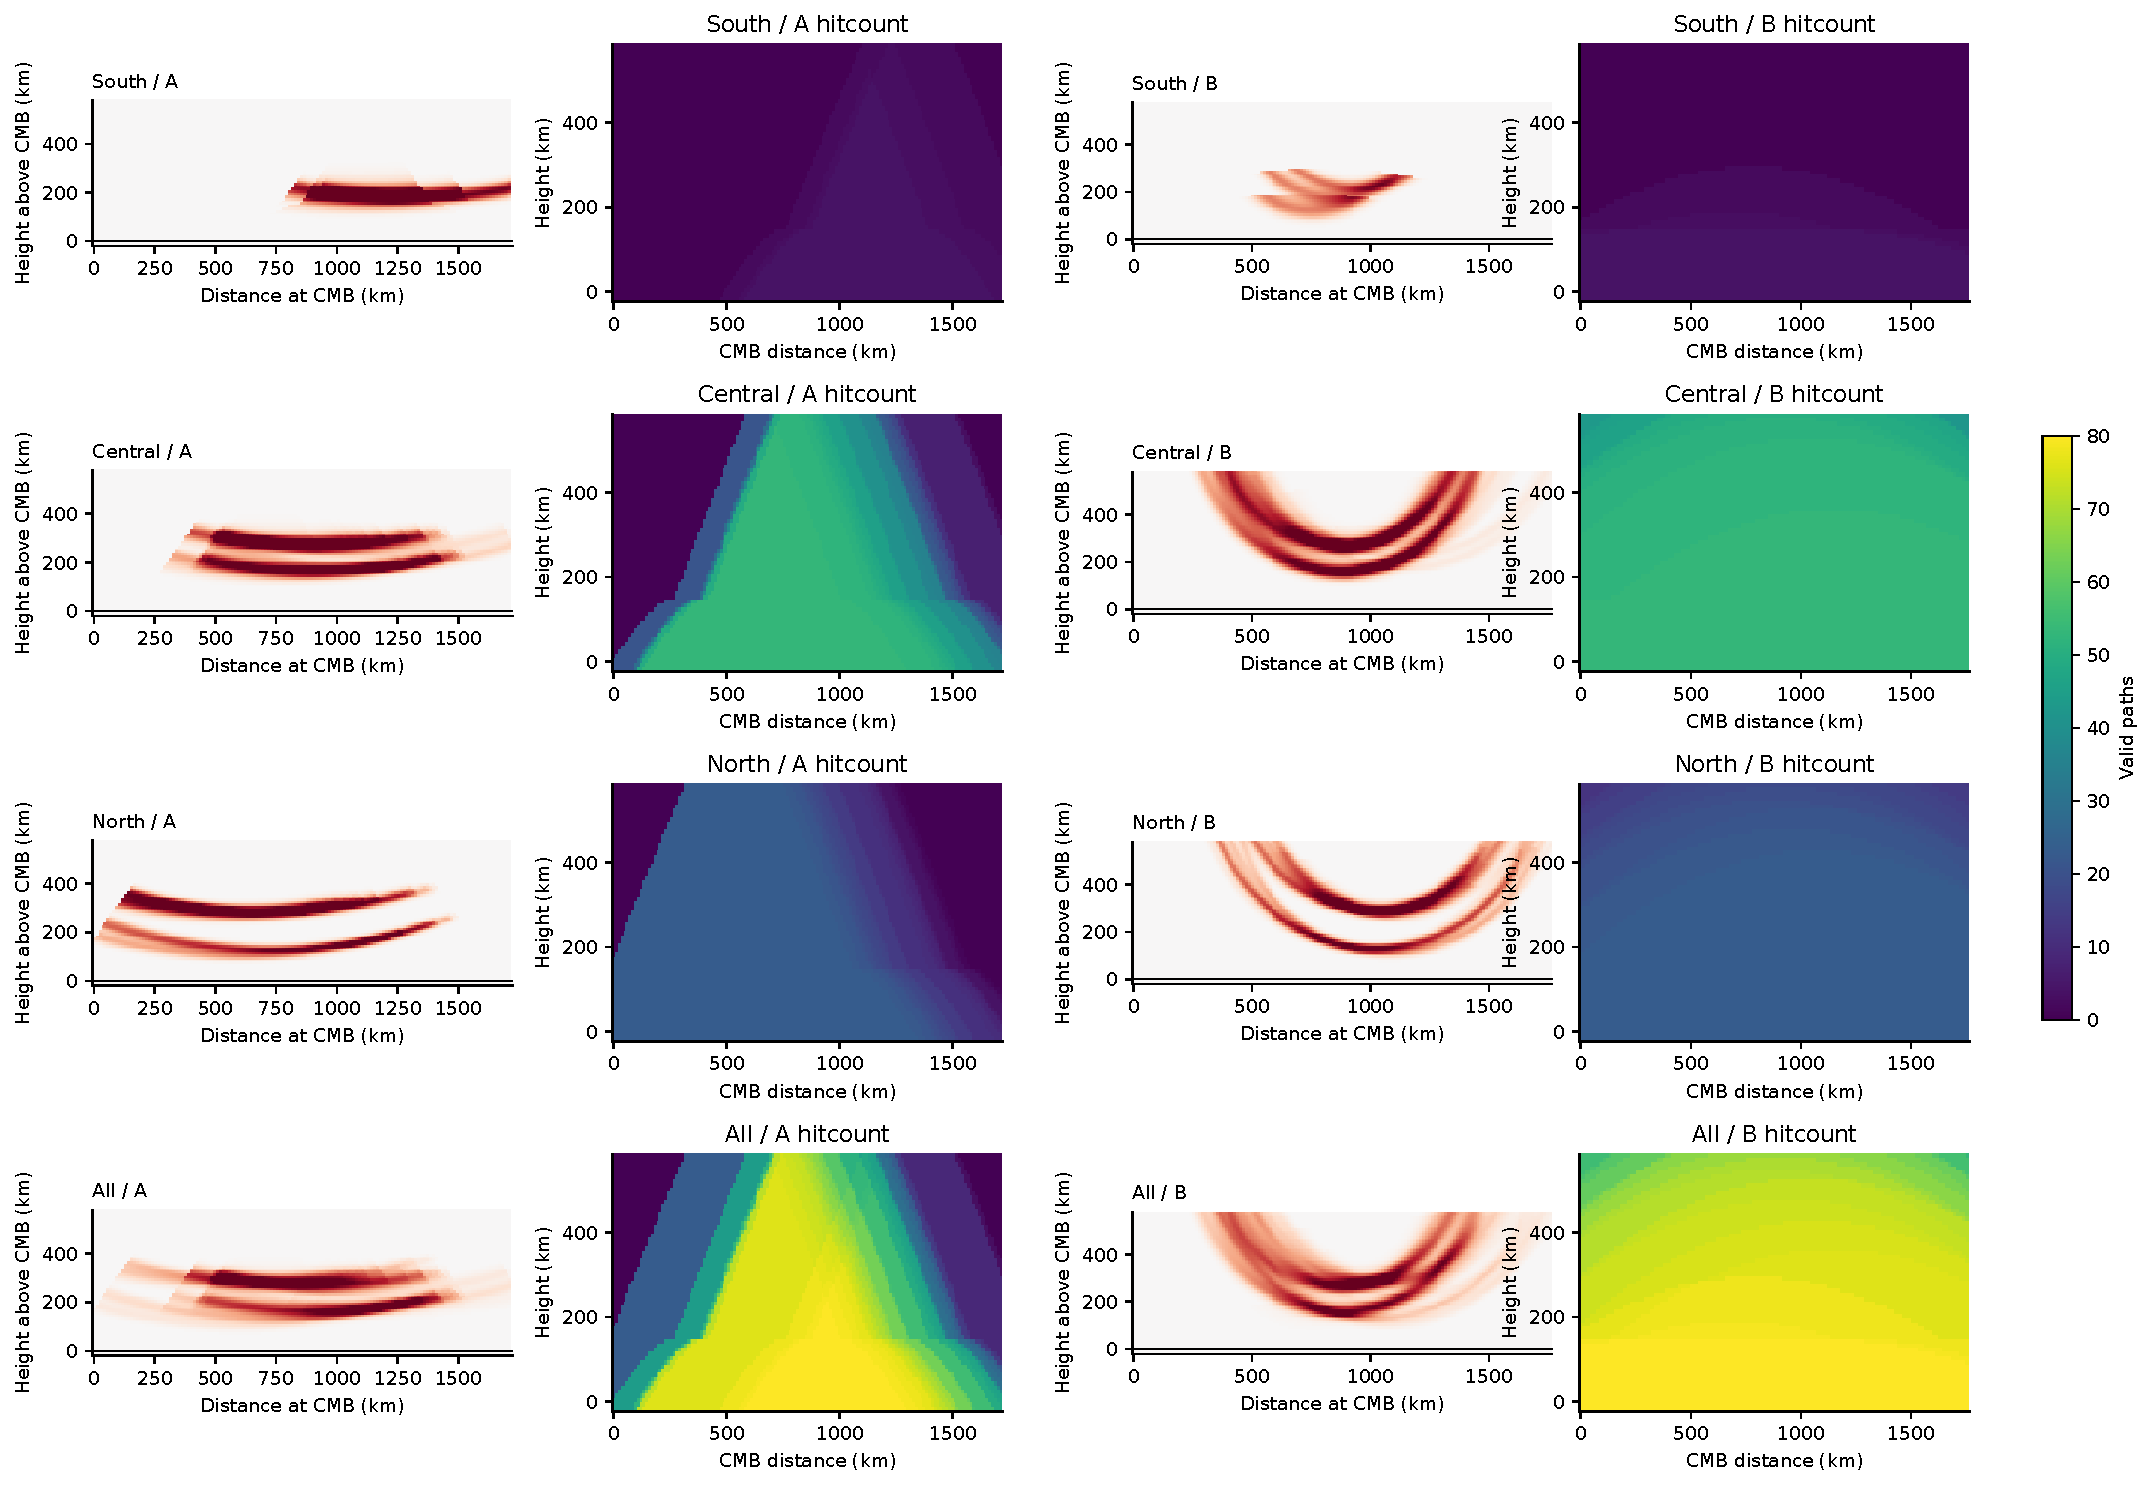
\includegraphics[width=.96\linewidth,height=.87\textheight,keepaspectratio]{figures/historical/supplement6.pdf}
\caption{historical; independent supplementary figure 6 counterpart. Definitions, assumptions, and panel status are given in the panel record. All numerical values come from saved arrays.}\end{figure}
\begin{figure}[p]\centering
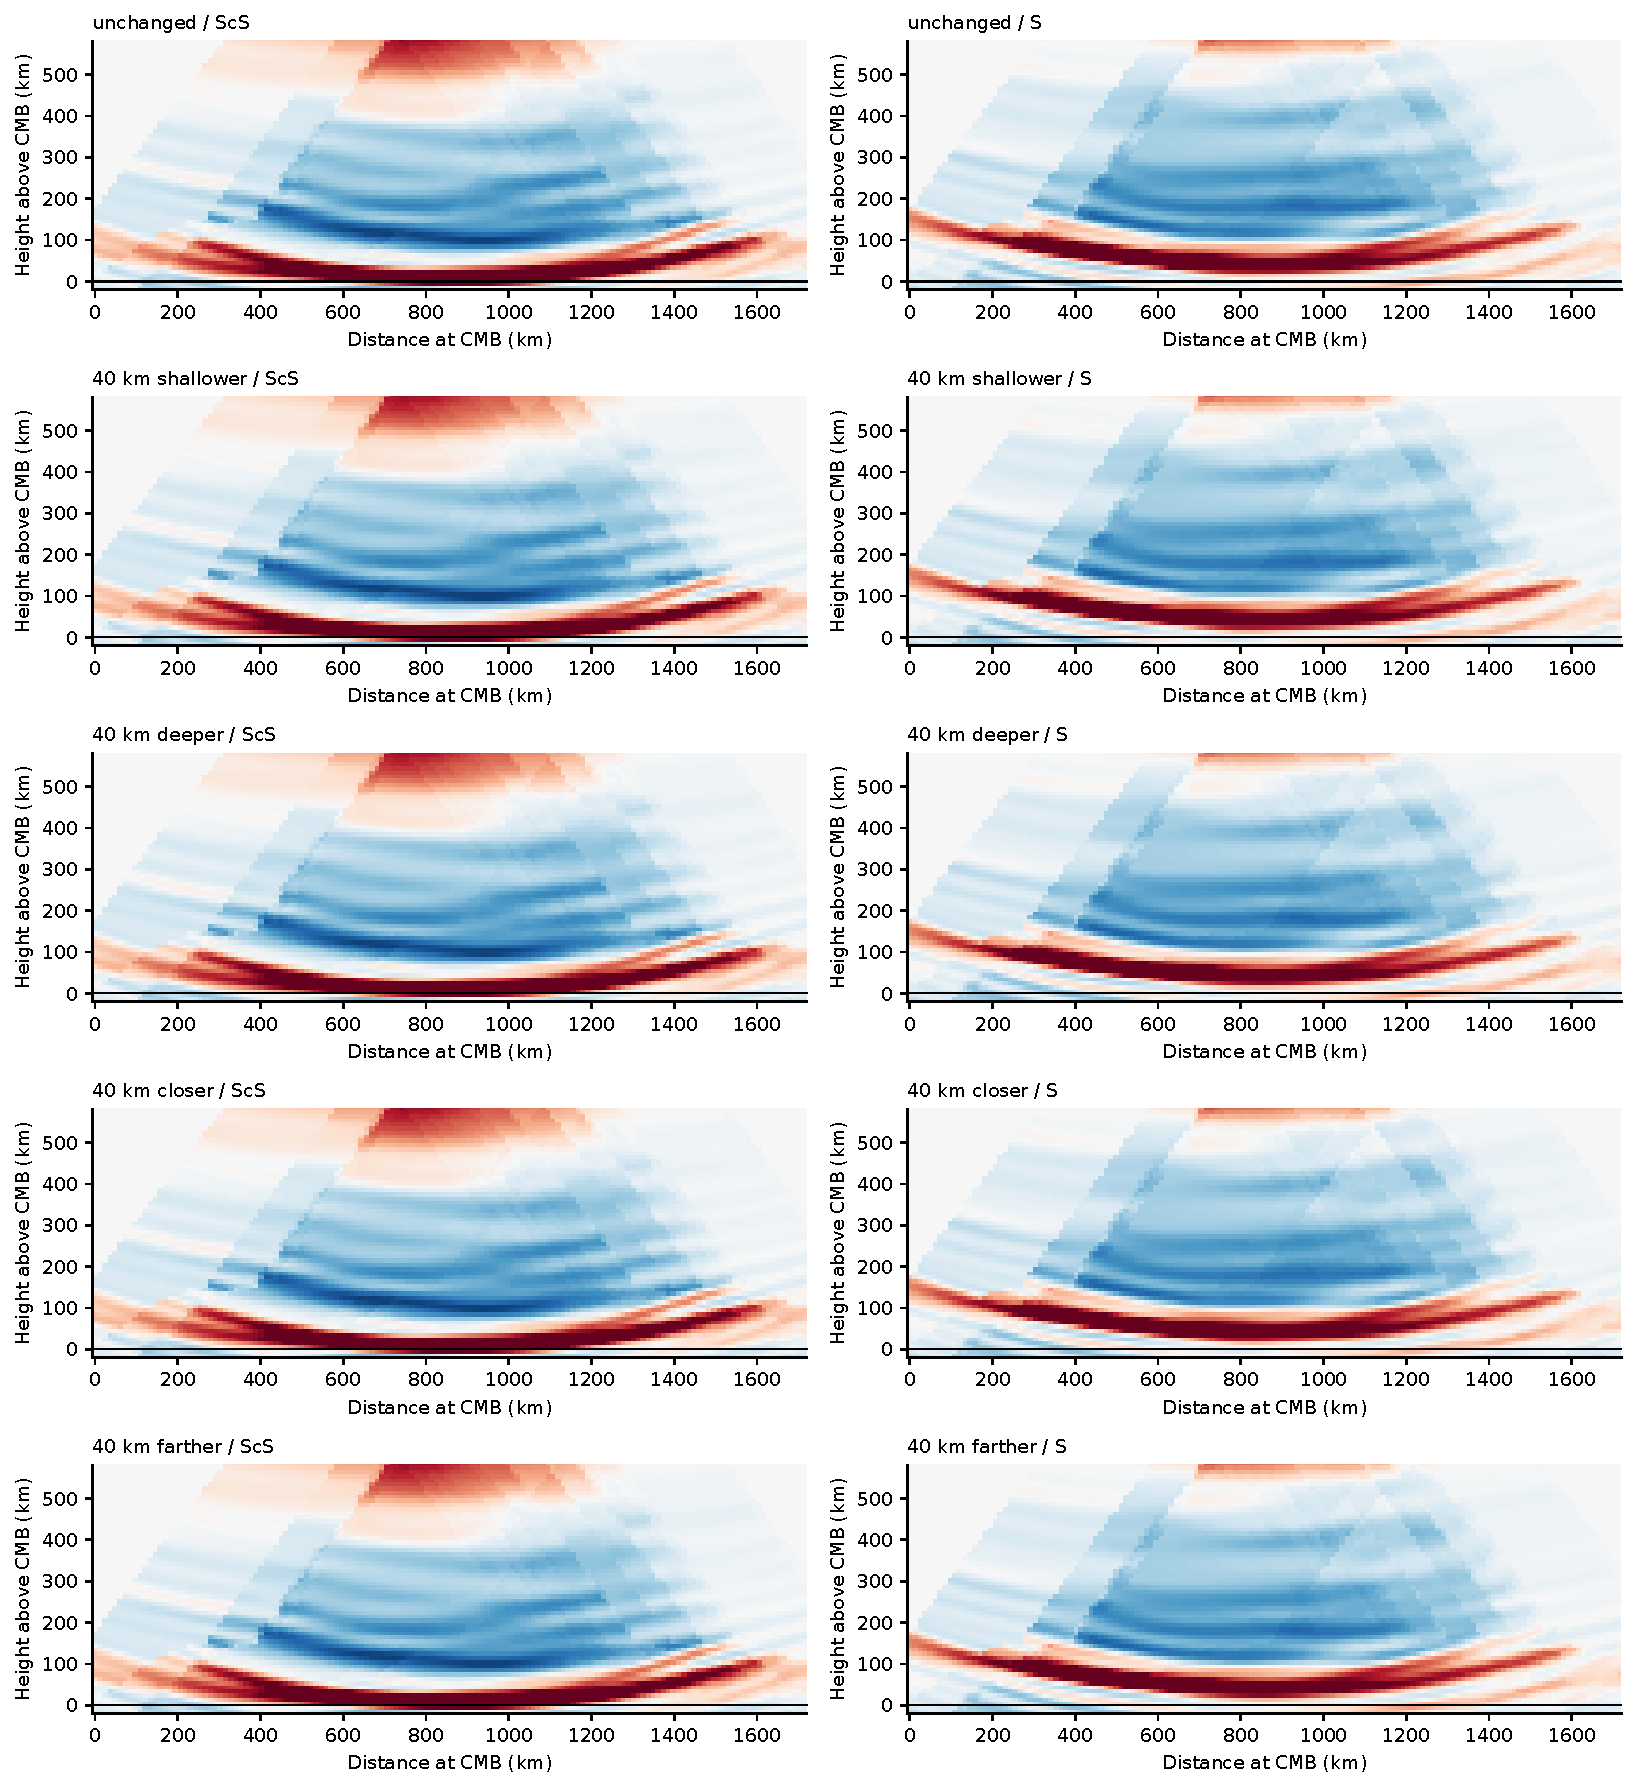
\includegraphics[width=.96\linewidth,height=.87\textheight,keepaspectratio]{figures/historical/supplement10.pdf}
\caption{historical; independent supplementary figure 10 counterpart. Definitions, assumptions, and panel status are given in the panel record. All numerical values come from saved arrays.}\end{figure}
\begin{figure}[p]\centering
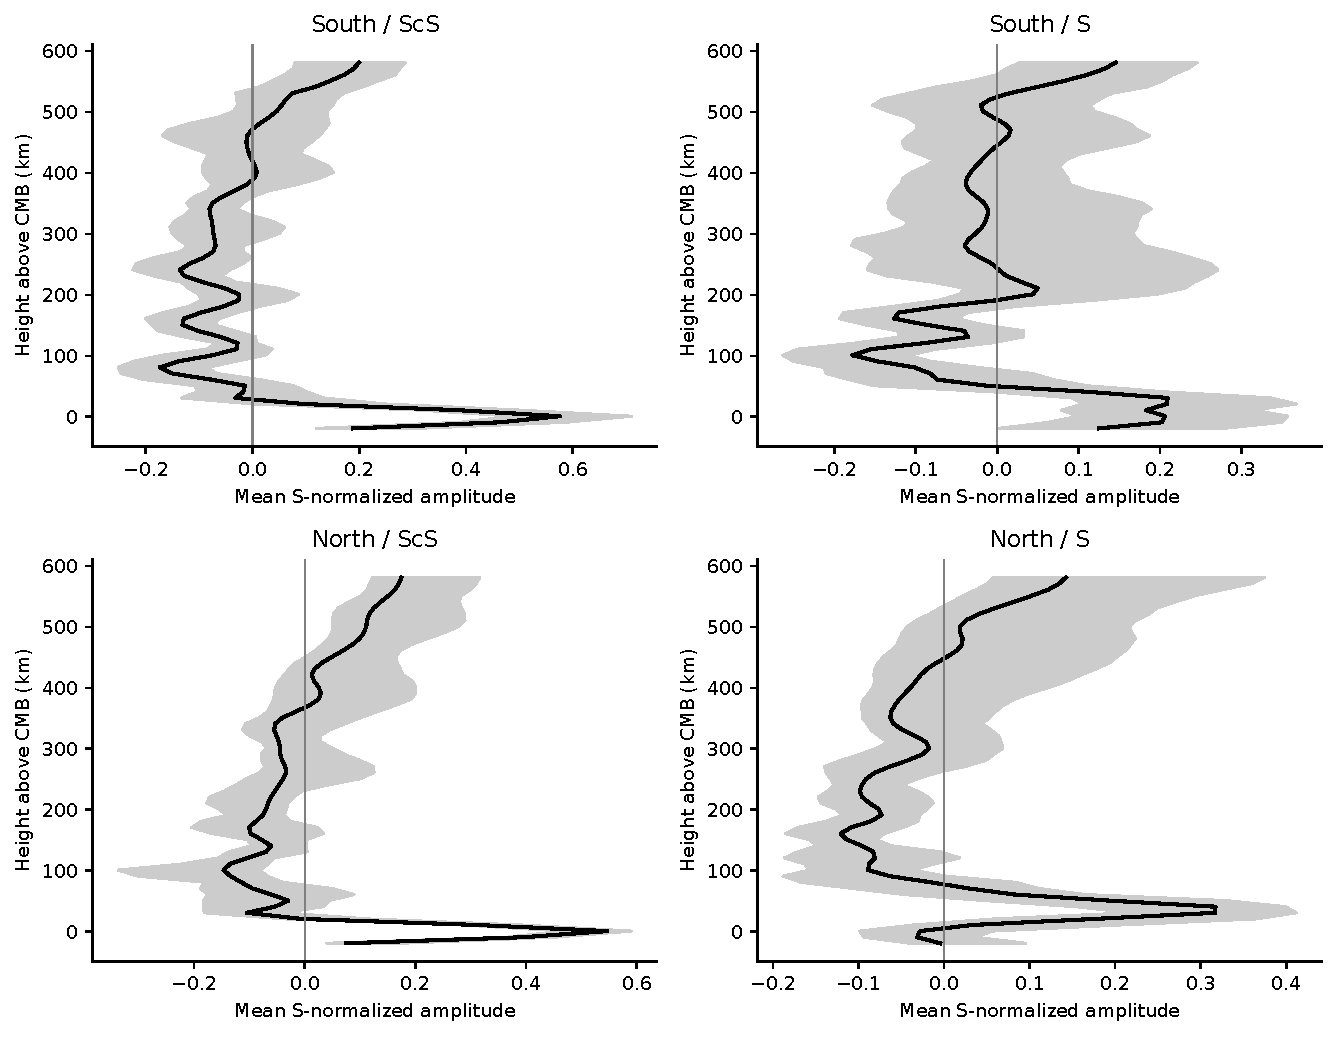
\includegraphics[width=.96\linewidth,height=.87\textheight,keepaspectratio]{figures/historical/supplement11.pdf}
\caption{historical; independent supplementary figure 11 counterpart. Definitions, assumptions, and panel status are given in the panel record. All numerical values come from saved arrays.}\end{figure}
\begin{figure}[p]\centering
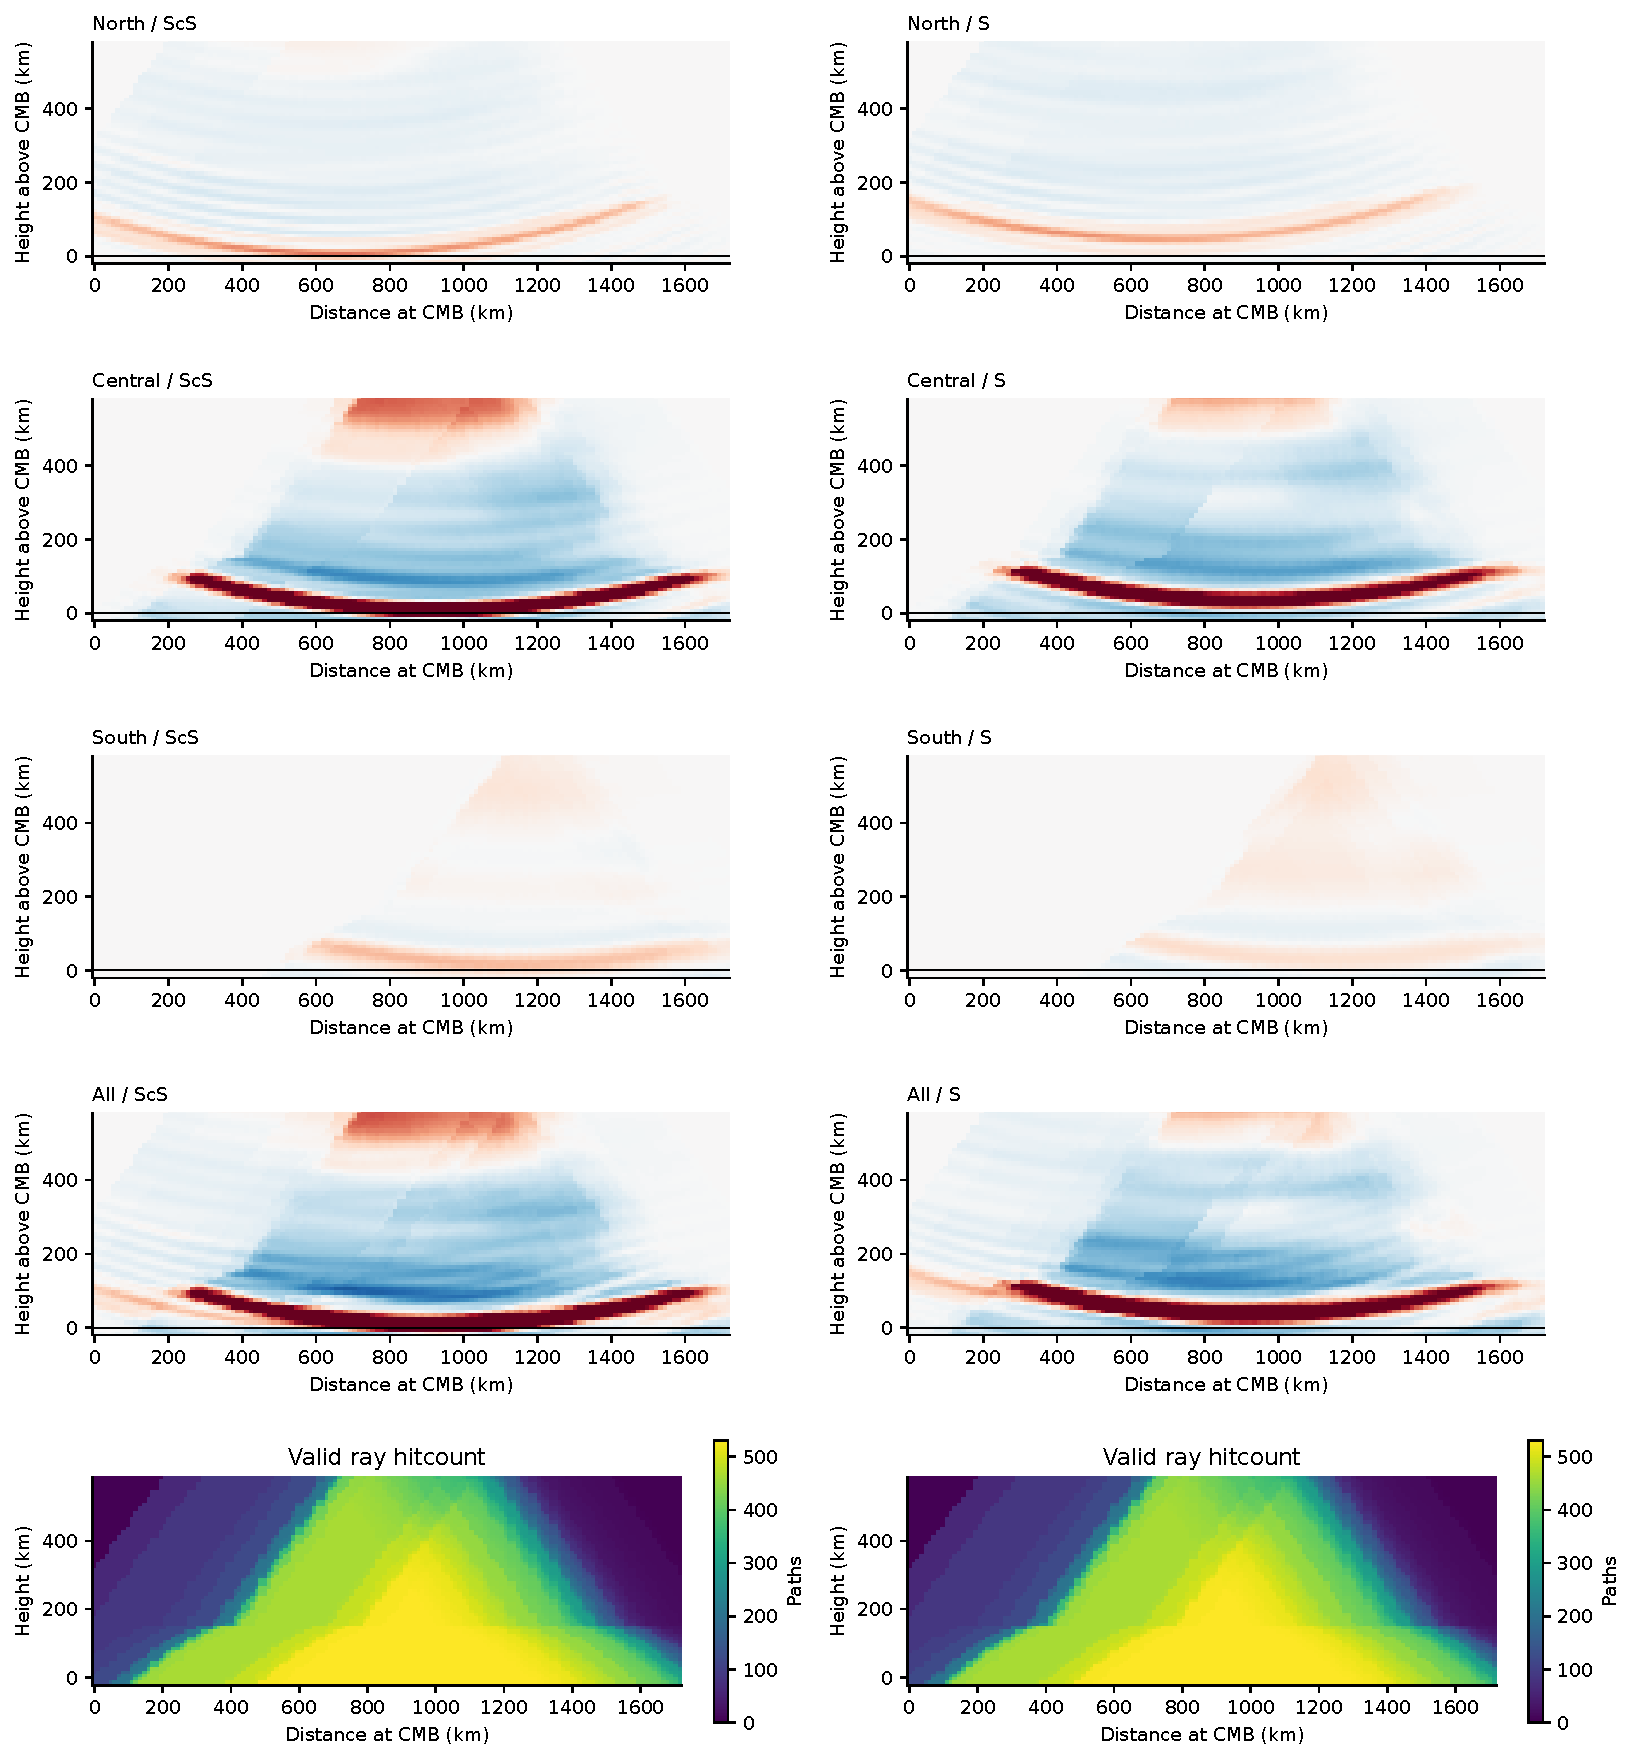
\includegraphics[width=.96\linewidth,height=.87\textheight,keepaspectratio]{figures/modern_same/supplement2.pdf}
\caption{modern\_same; independent supplementary figure 2 counterpart. Definitions, assumptions, and panel status are given in the panel record. All numerical values come from saved arrays.}\end{figure}
\begin{figure}[p]\centering
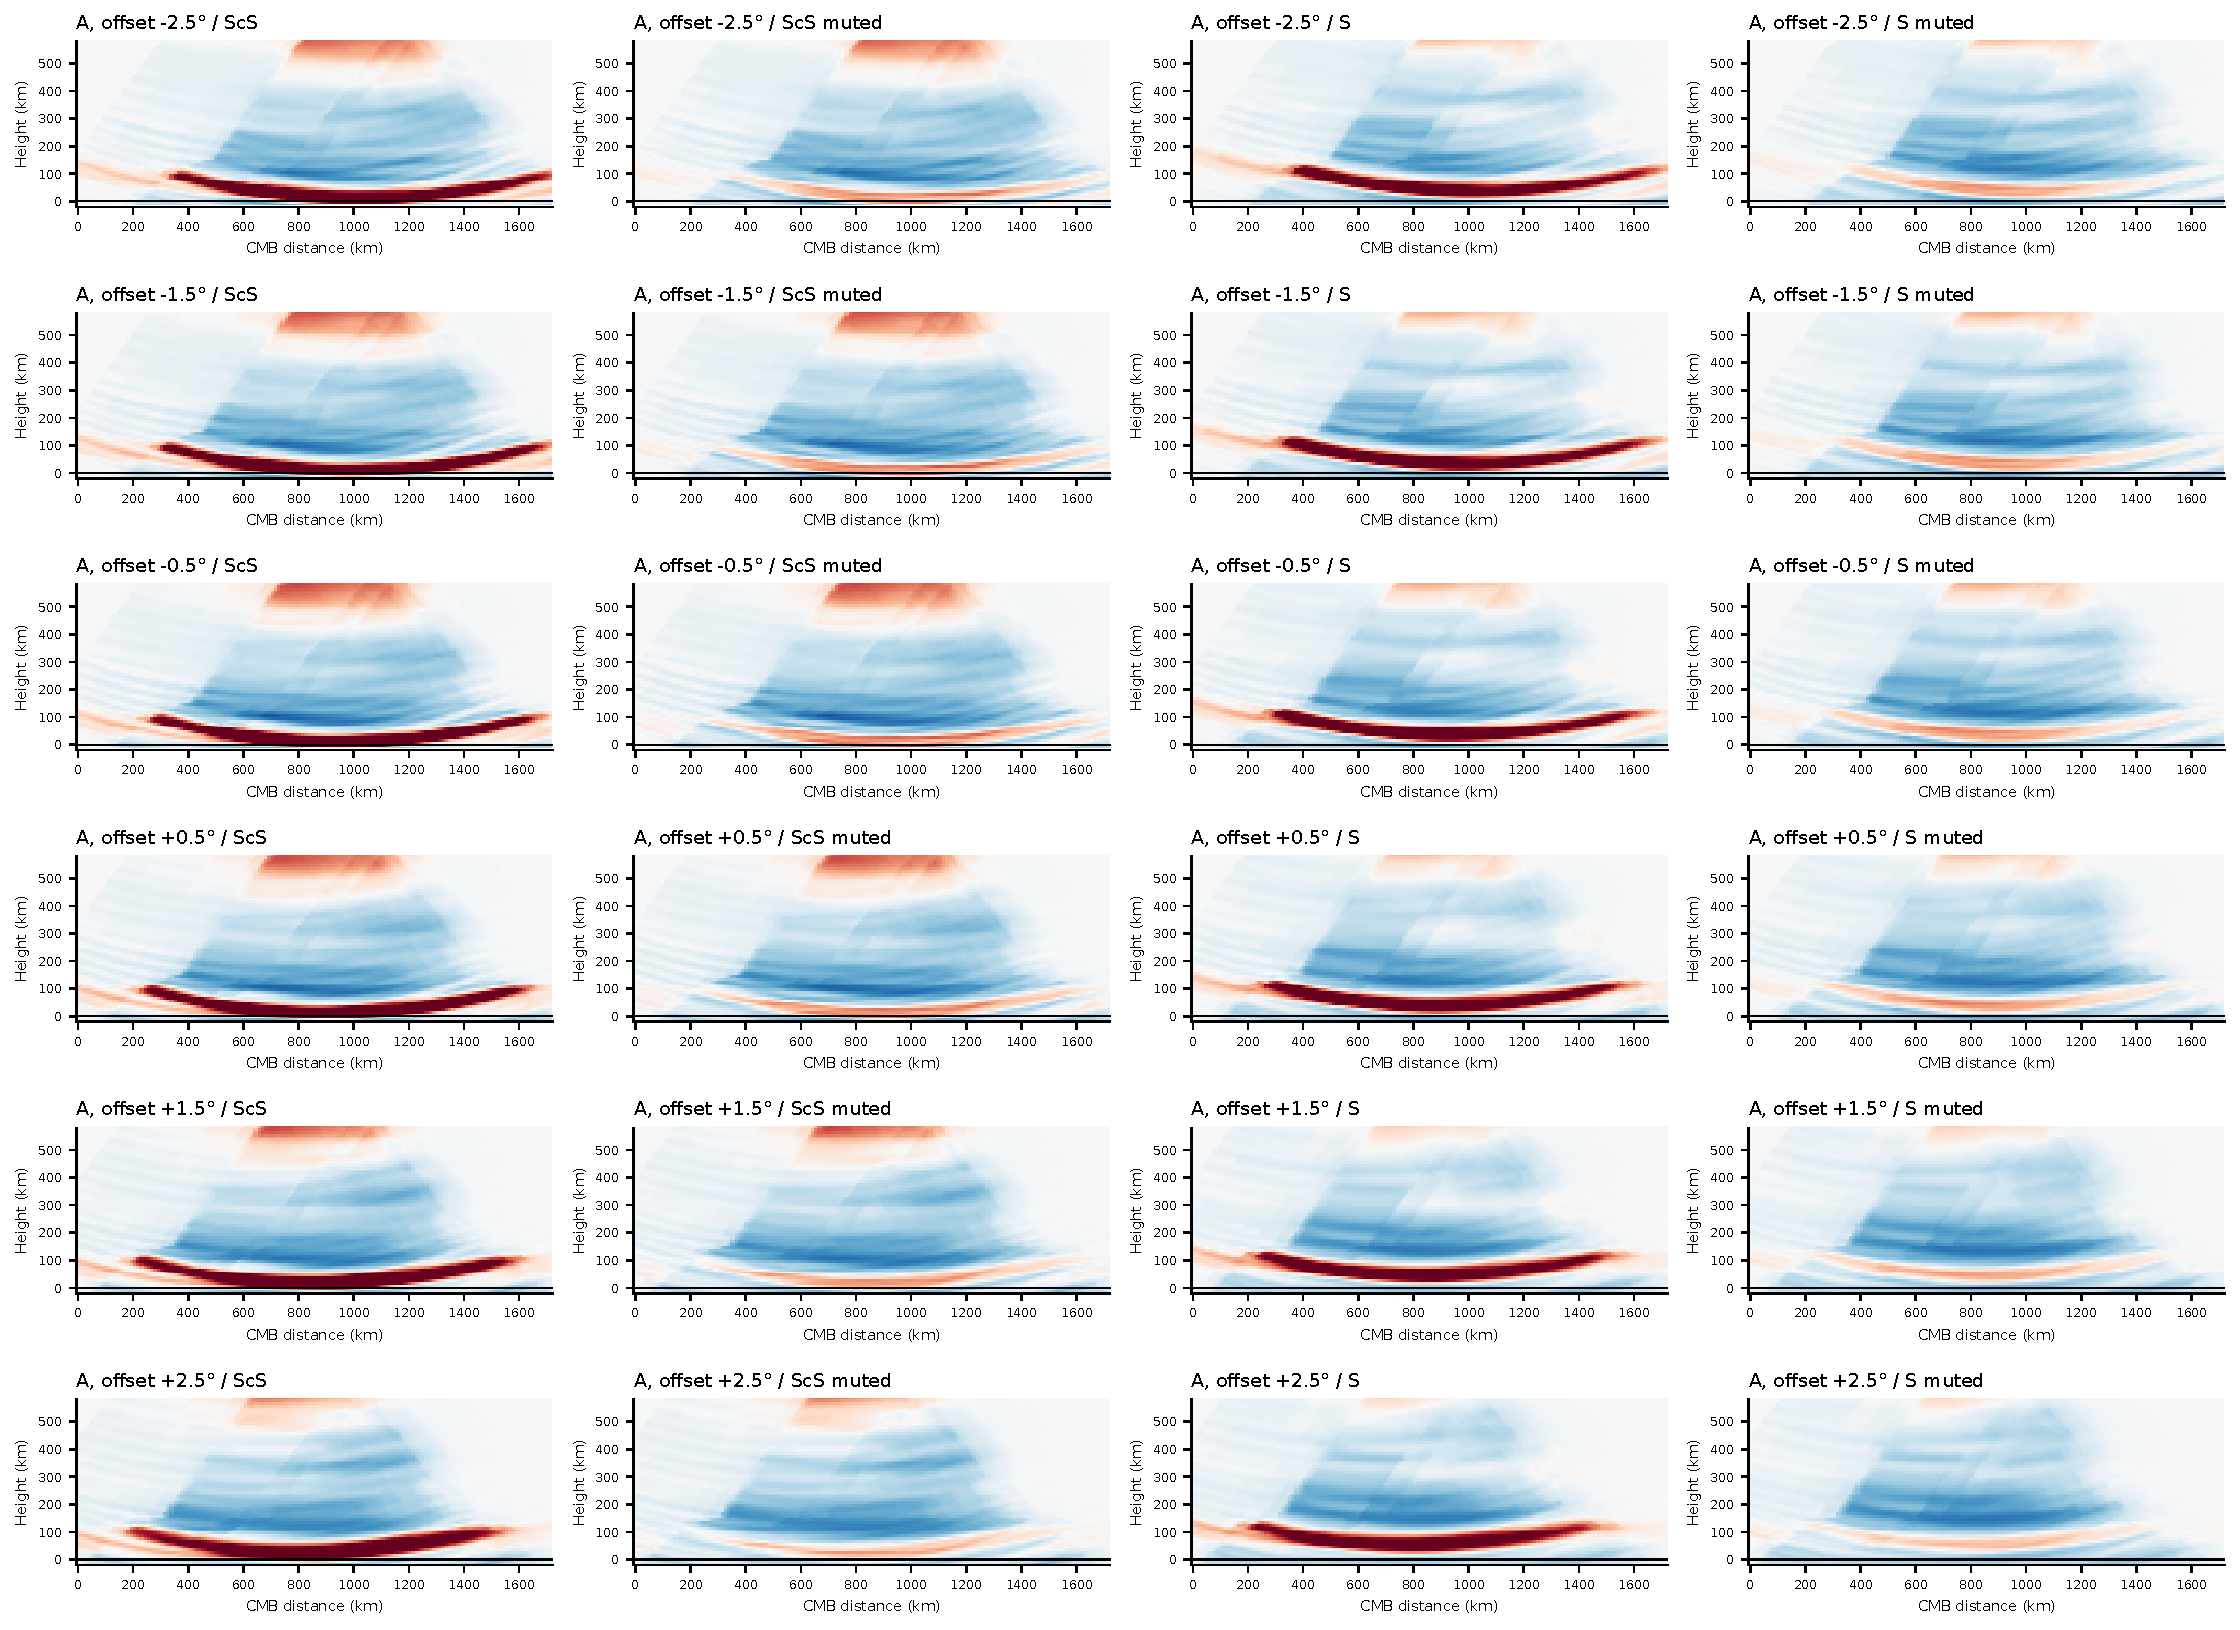
\includegraphics[width=.96\linewidth,height=.87\textheight,keepaspectratio]{figures/modern_same/supplement3a.pdf}
\caption{modern\_same; independent supplementary figure 3a counterpart. Definitions, assumptions, and panel status are given in the panel record. All numerical values come from saved arrays.}\end{figure}
\begin{figure}[p]\centering
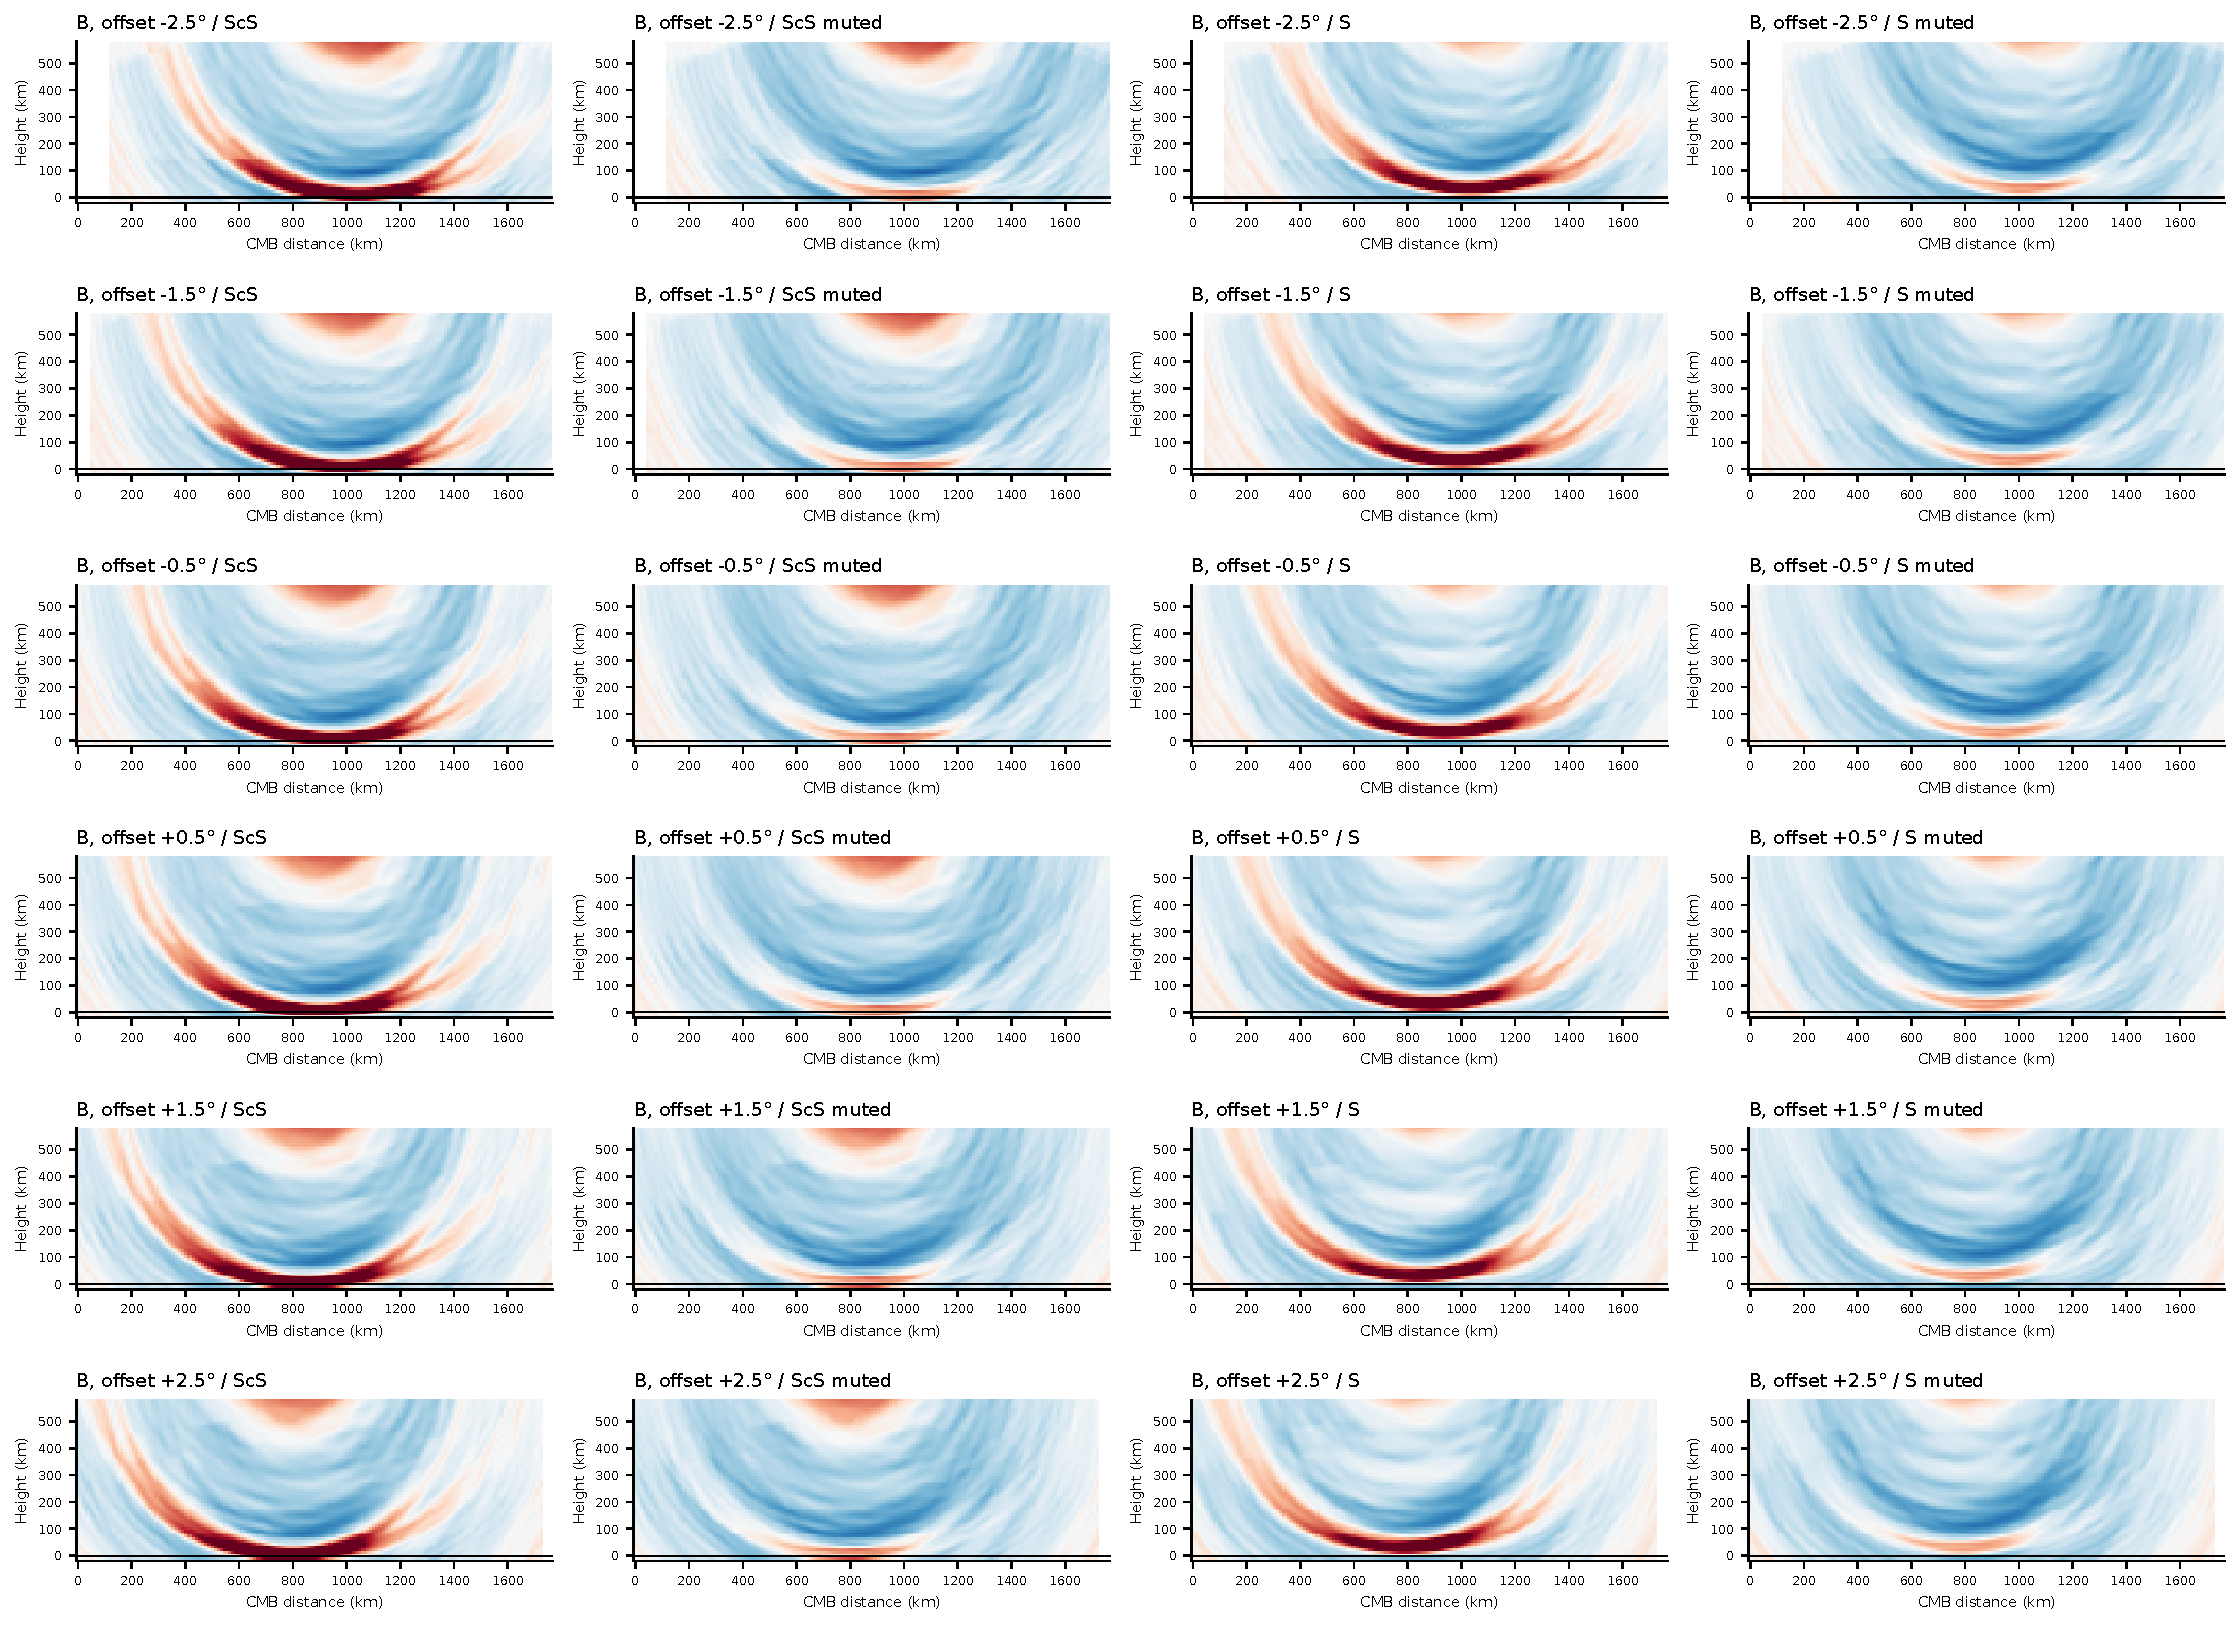
\includegraphics[width=.96\linewidth,height=.87\textheight,keepaspectratio]{figures/modern_same/supplement3b.pdf}
\caption{modern\_same; independent supplementary figure 3b counterpart. Definitions, assumptions, and panel status are given in the panel record. All numerical values come from saved arrays.}\end{figure}
\begin{figure}[p]\centering
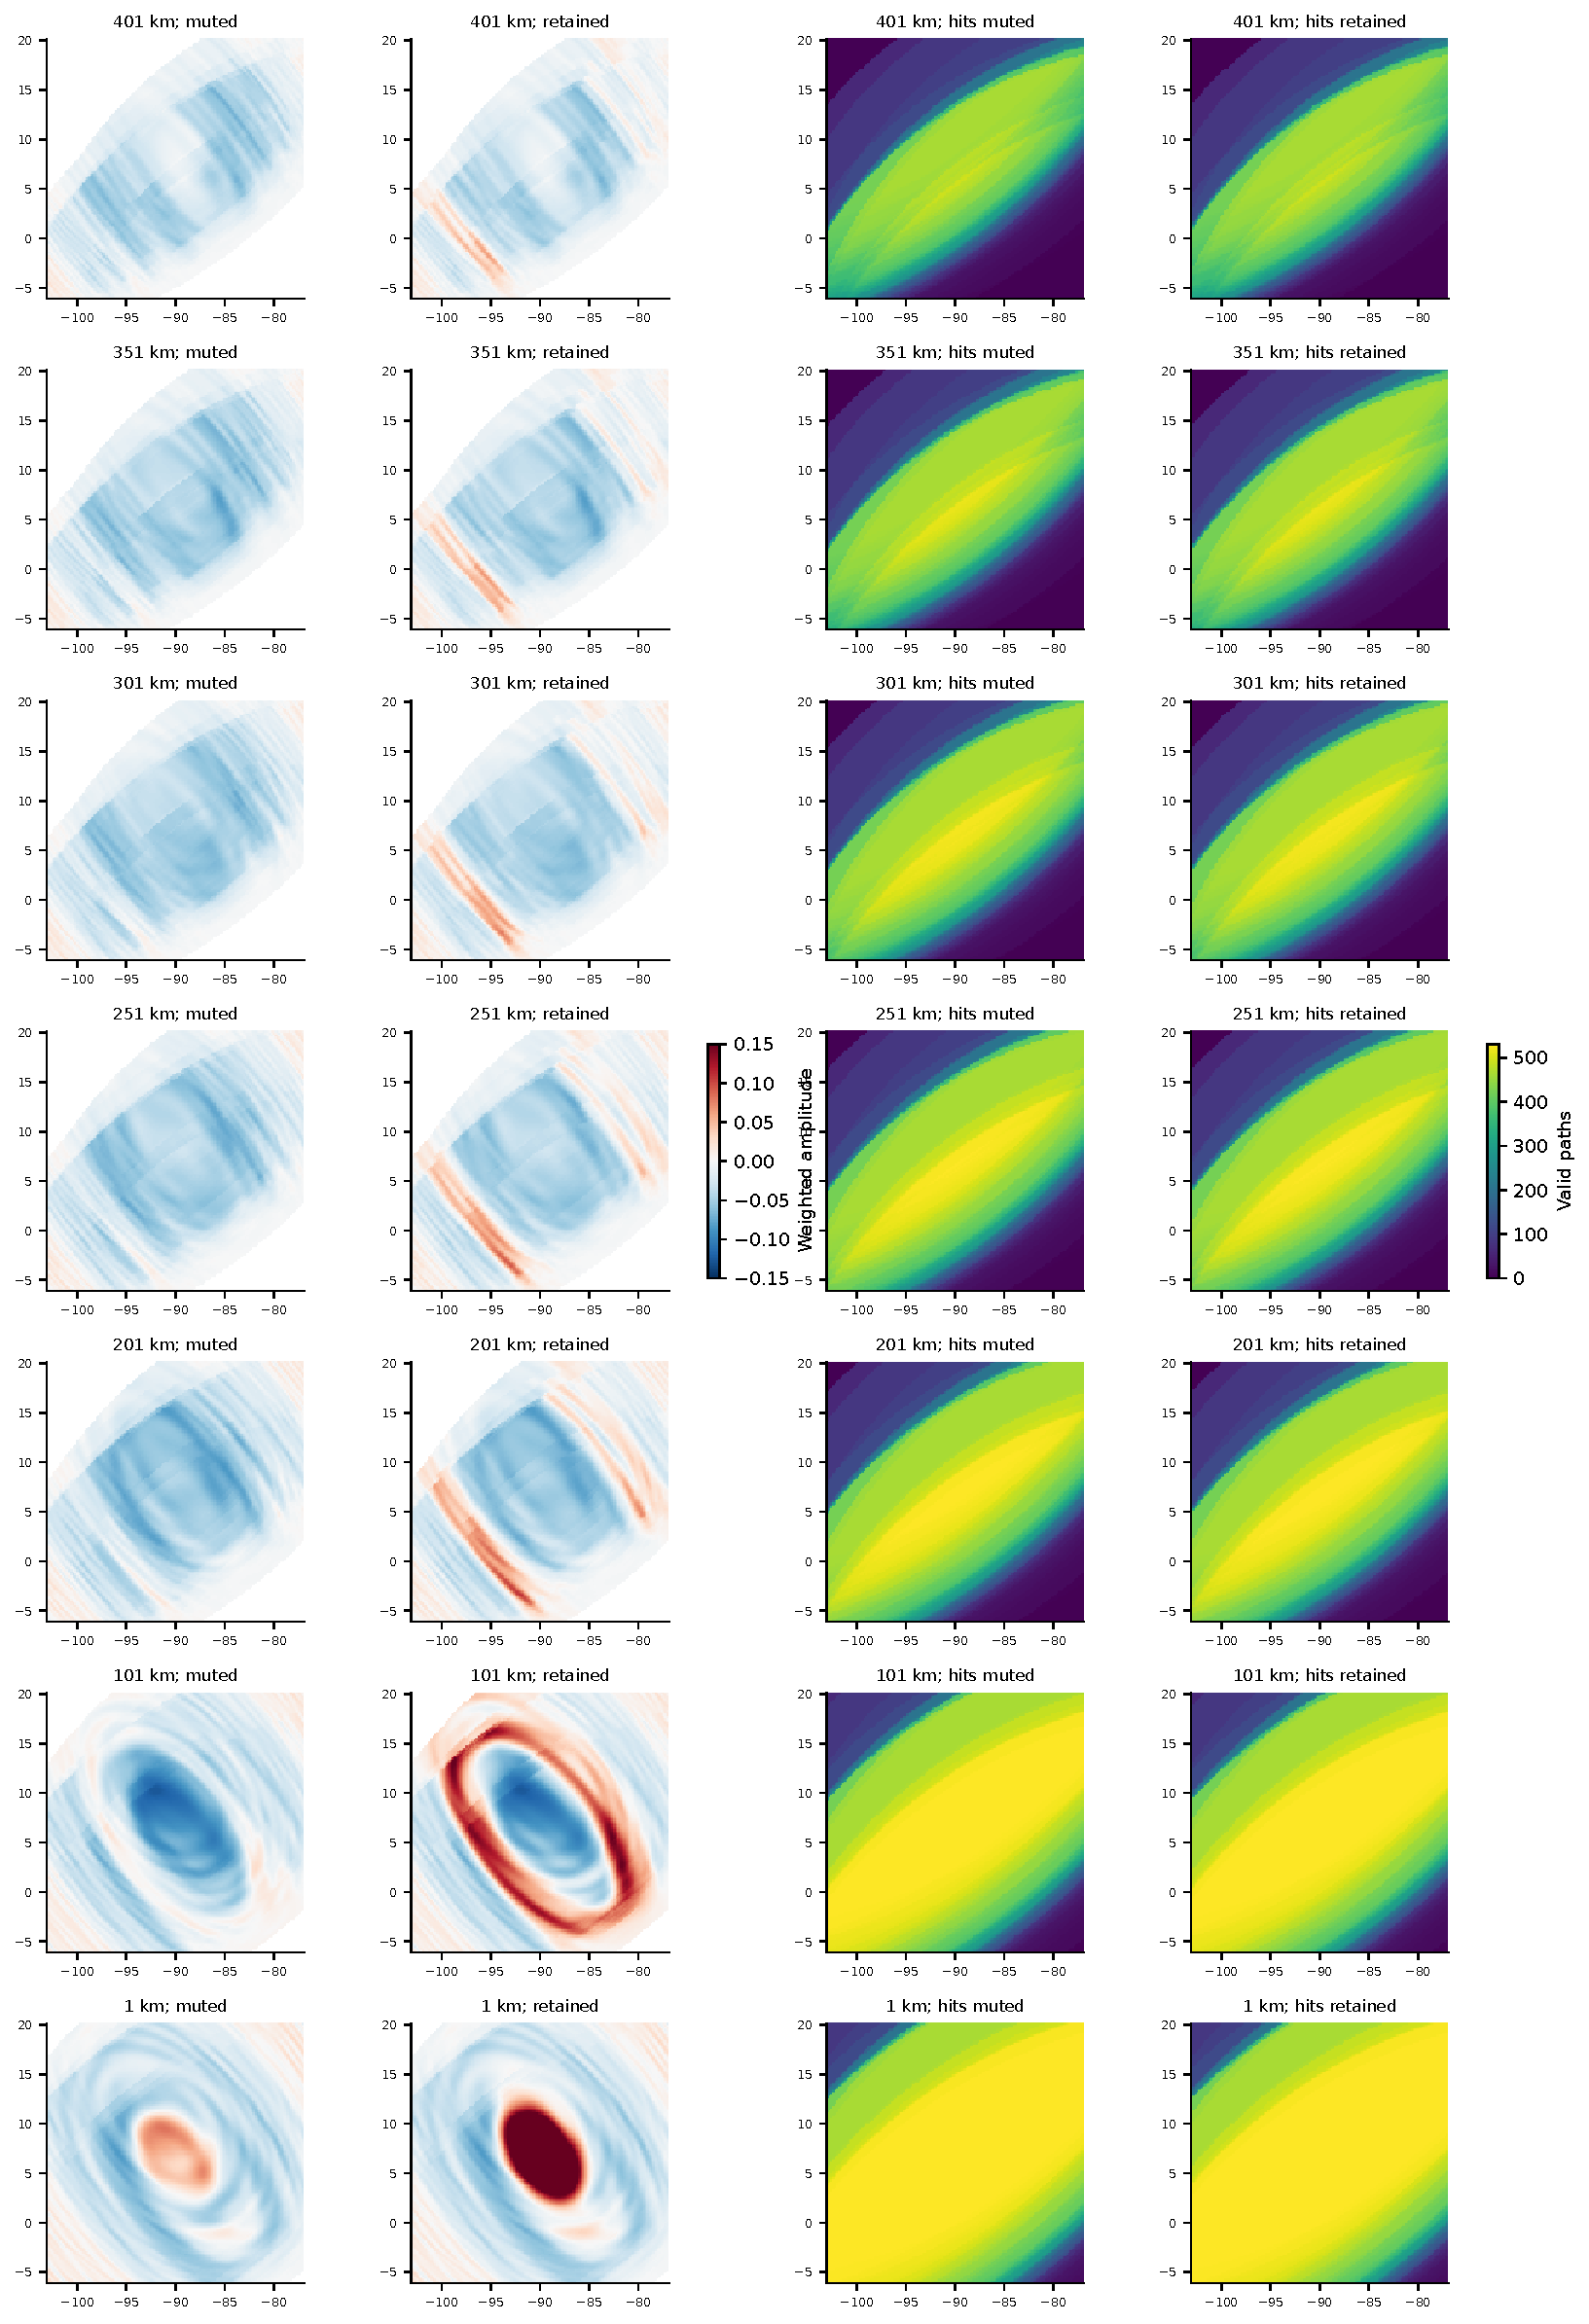
\includegraphics[width=.96\linewidth,height=.87\textheight,keepaspectratio]{figures/modern_same/supplement5.pdf}
\caption{modern\_same; independent supplementary figure 5 counterpart. Definitions, assumptions, and panel status are given in the panel record. All numerical values come from saved arrays.}\end{figure}
\begin{figure}[p]\centering
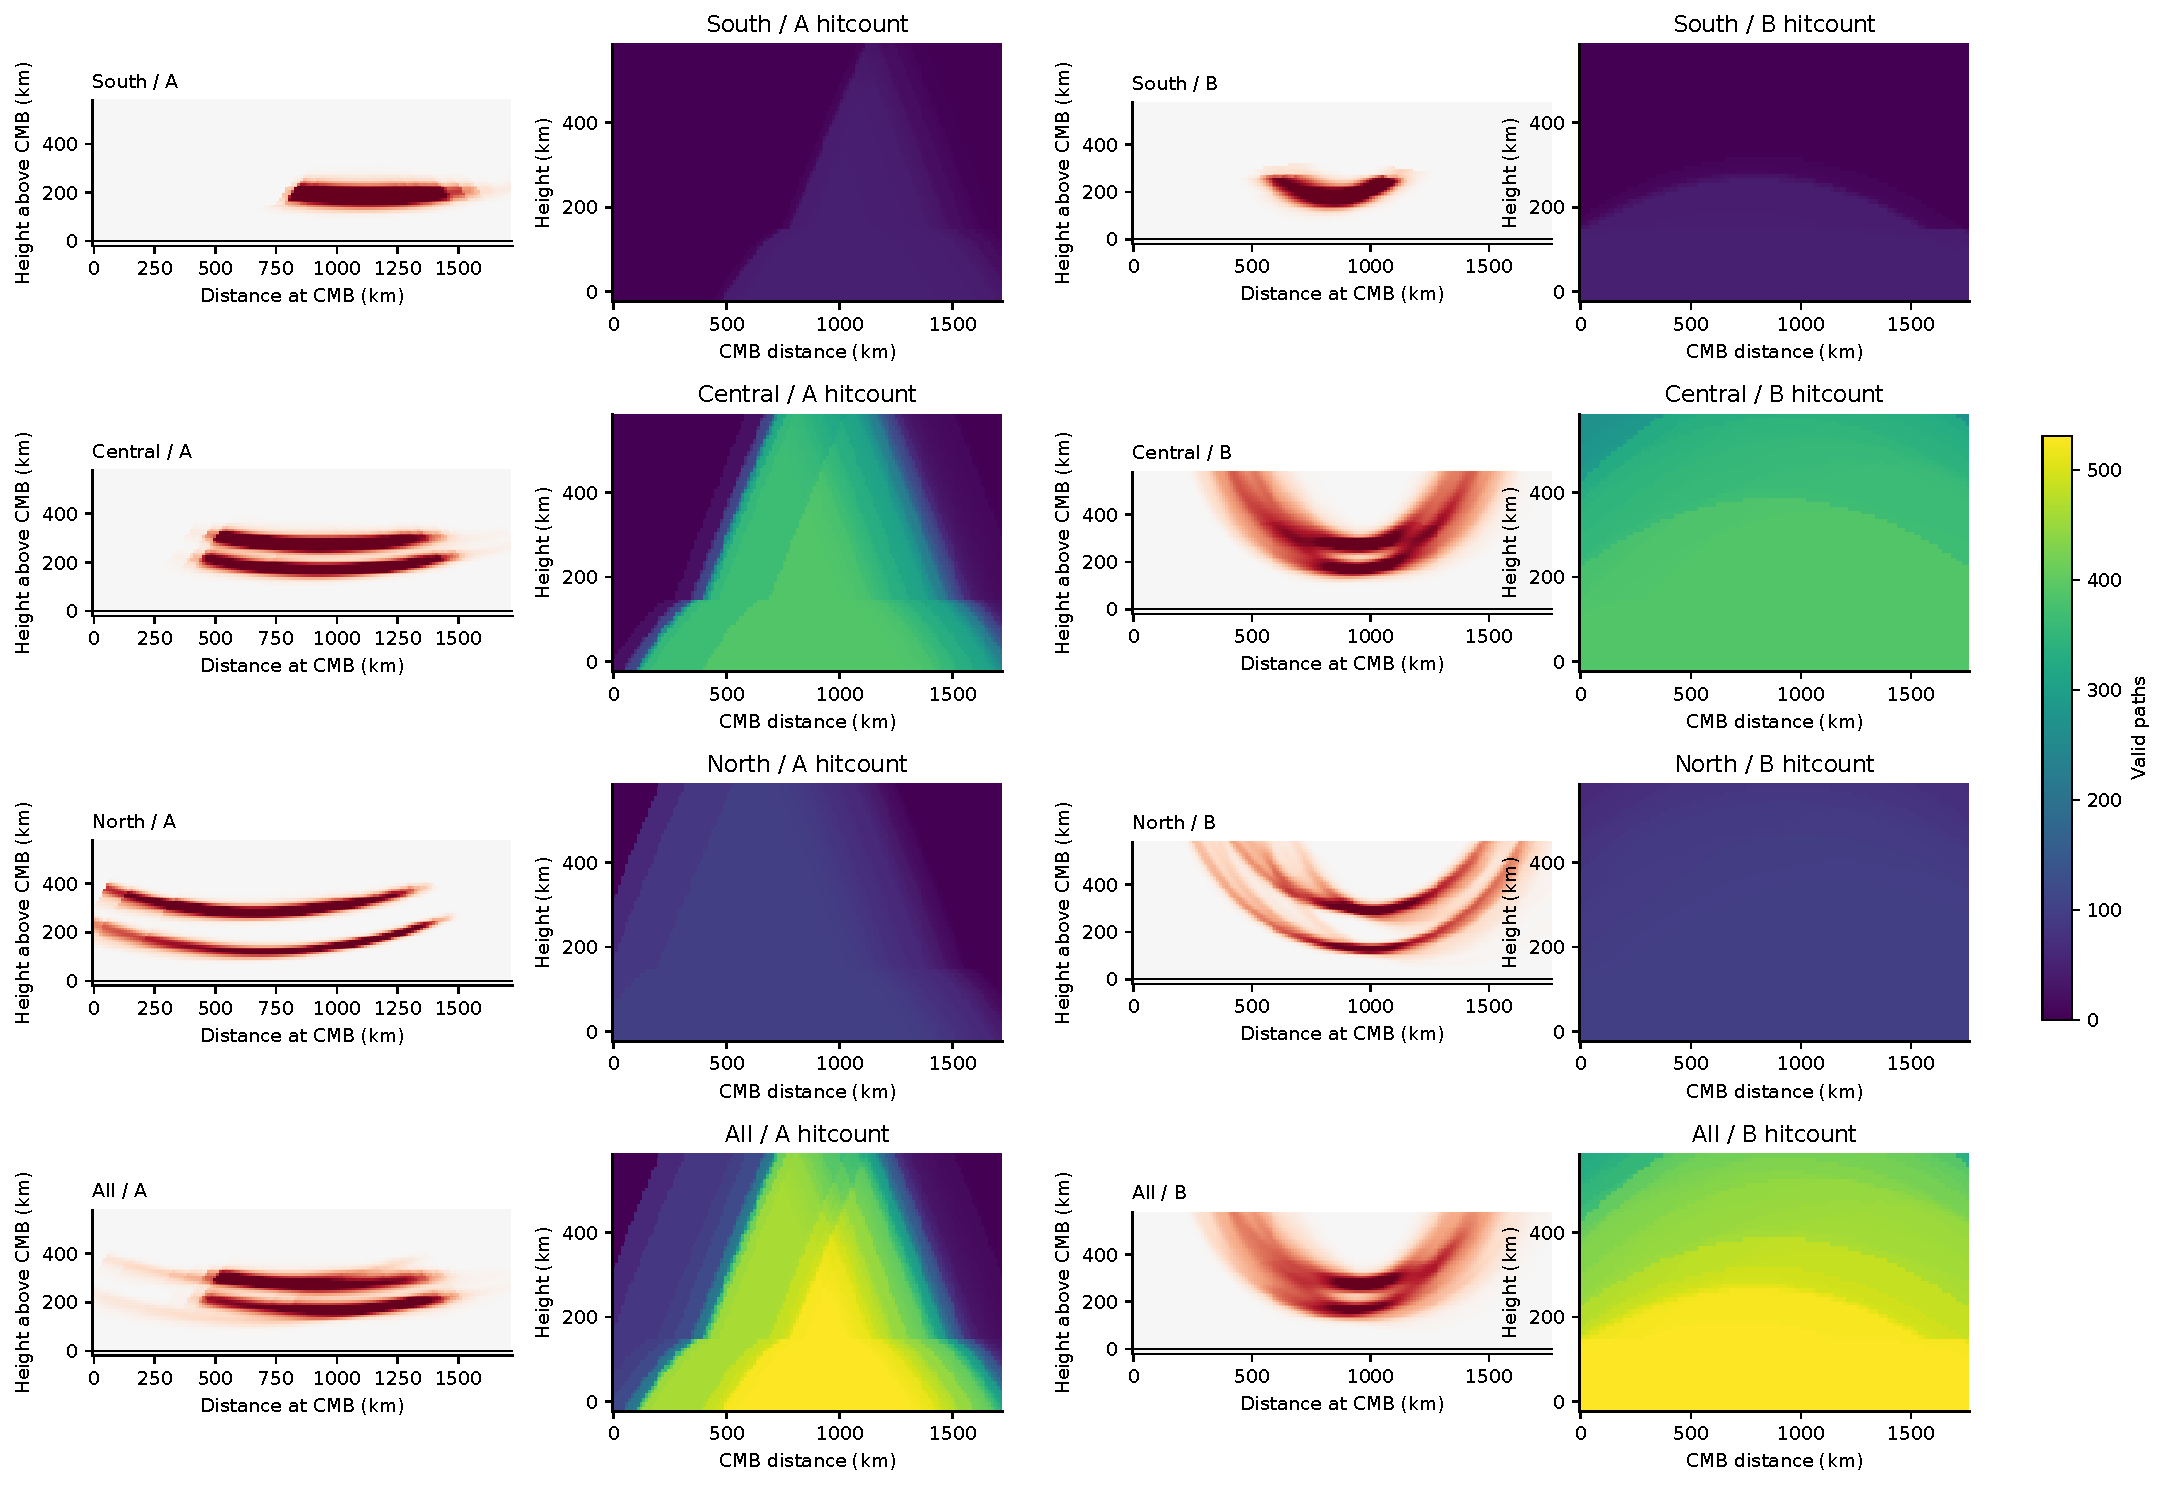
\includegraphics[width=.96\linewidth,height=.87\textheight,keepaspectratio]{figures/modern_same/supplement6.pdf}
\caption{modern\_same; independent supplementary figure 6 counterpart. Definitions, assumptions, and panel status are given in the panel record. All numerical values come from saved arrays.}\end{figure}
\begin{figure}[p]\centering
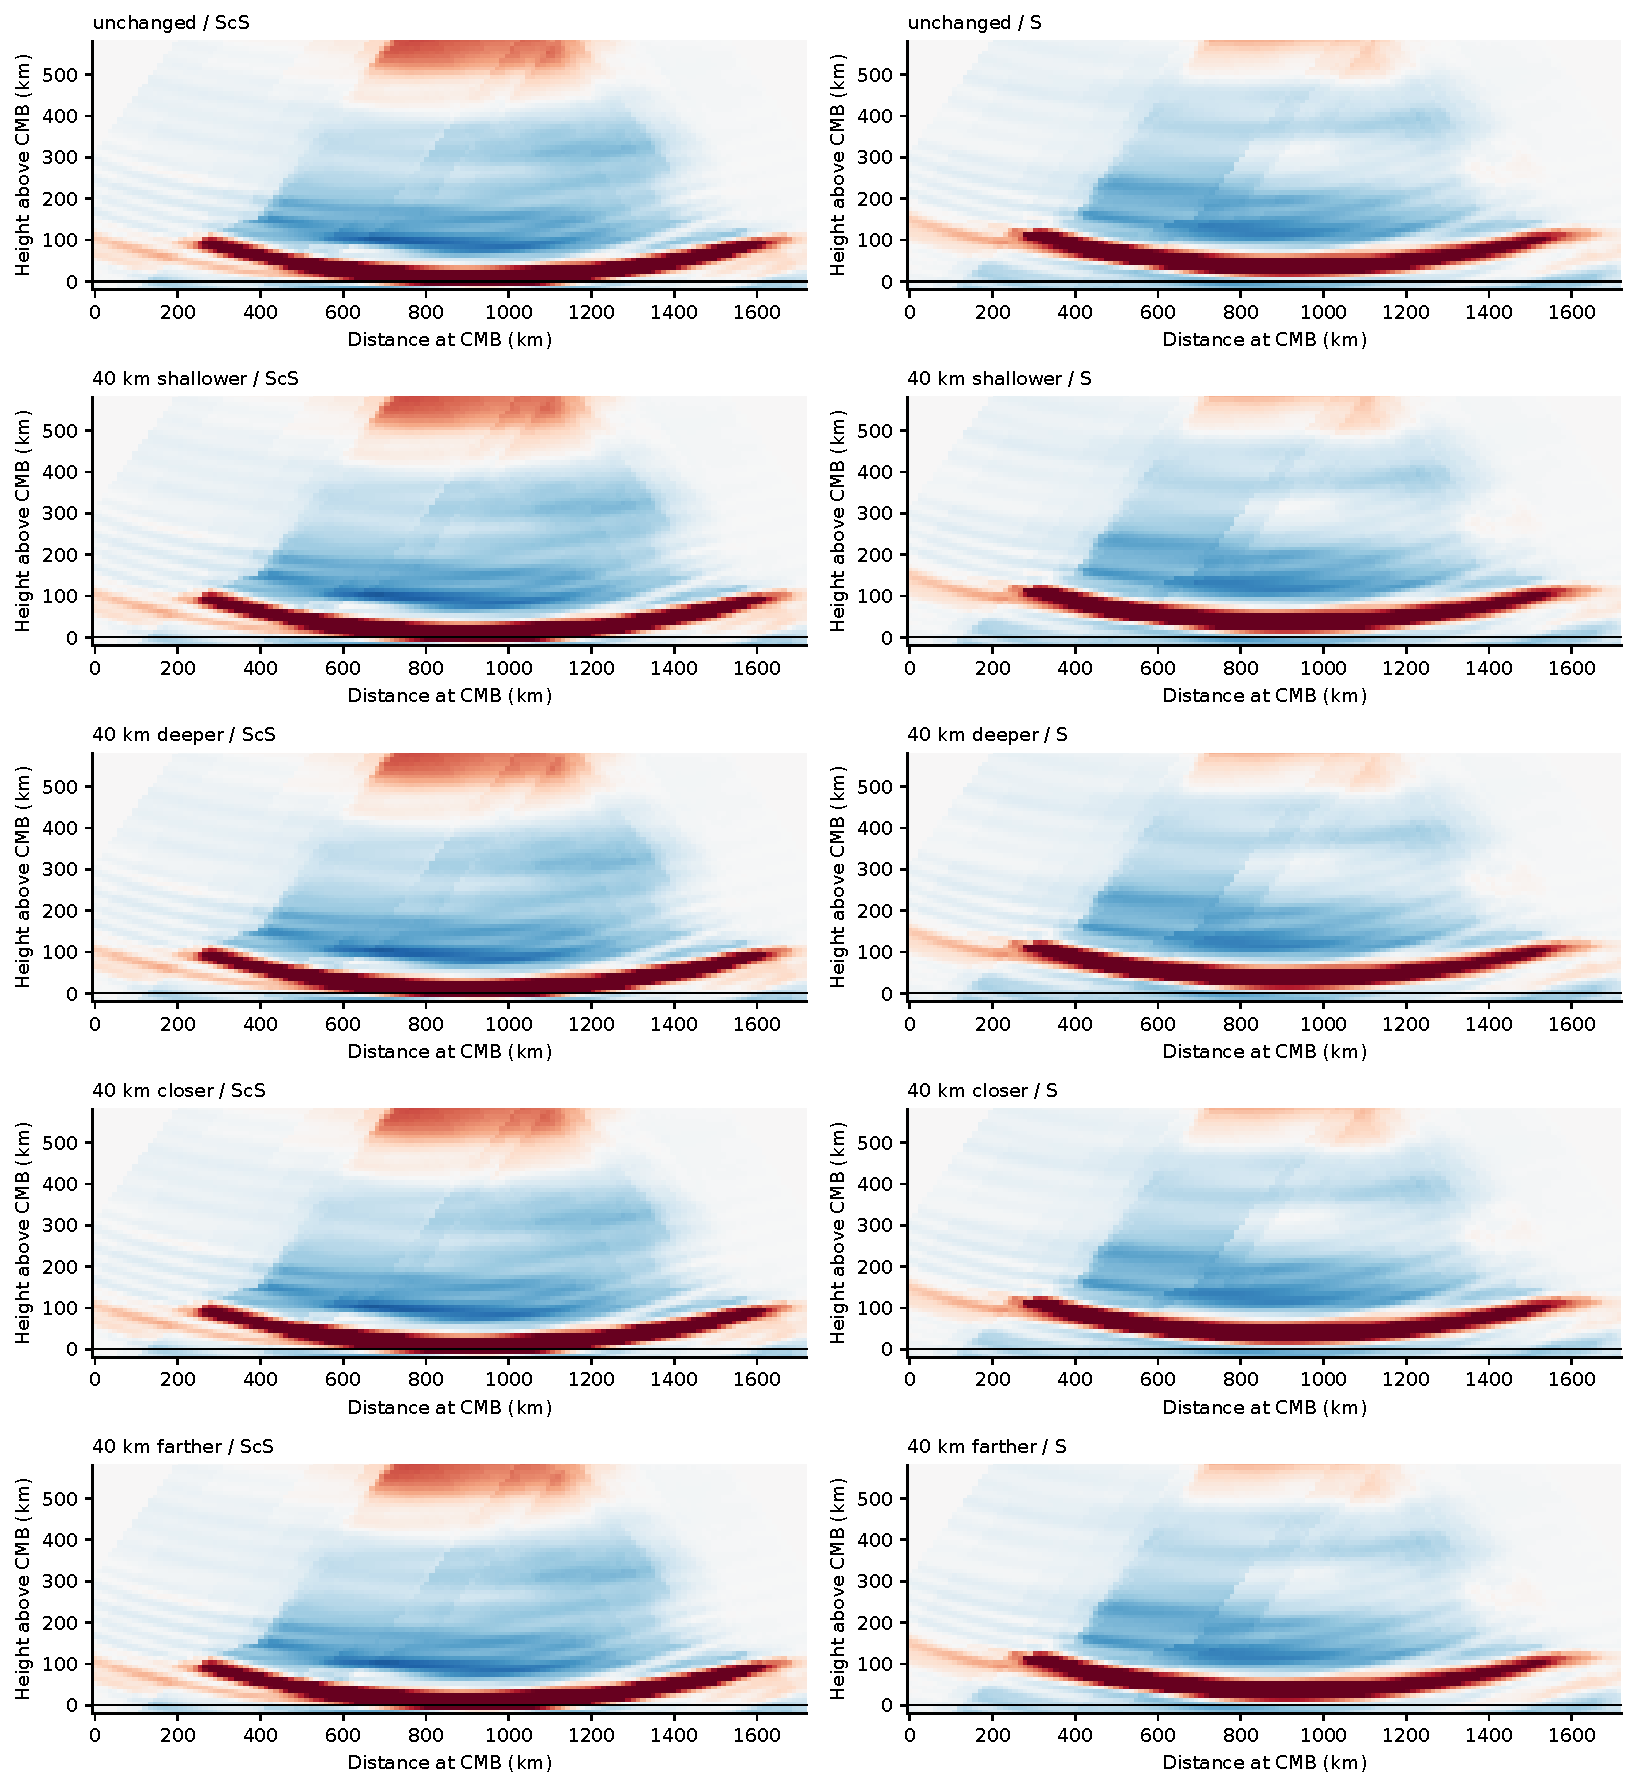
\includegraphics[width=.96\linewidth,height=.87\textheight,keepaspectratio]{figures/modern_same/supplement10.pdf}
\caption{modern\_same; independent supplementary figure 10 counterpart. Definitions, assumptions, and panel status are given in the panel record. All numerical values come from saved arrays.}\end{figure}
\begin{figure}[p]\centering
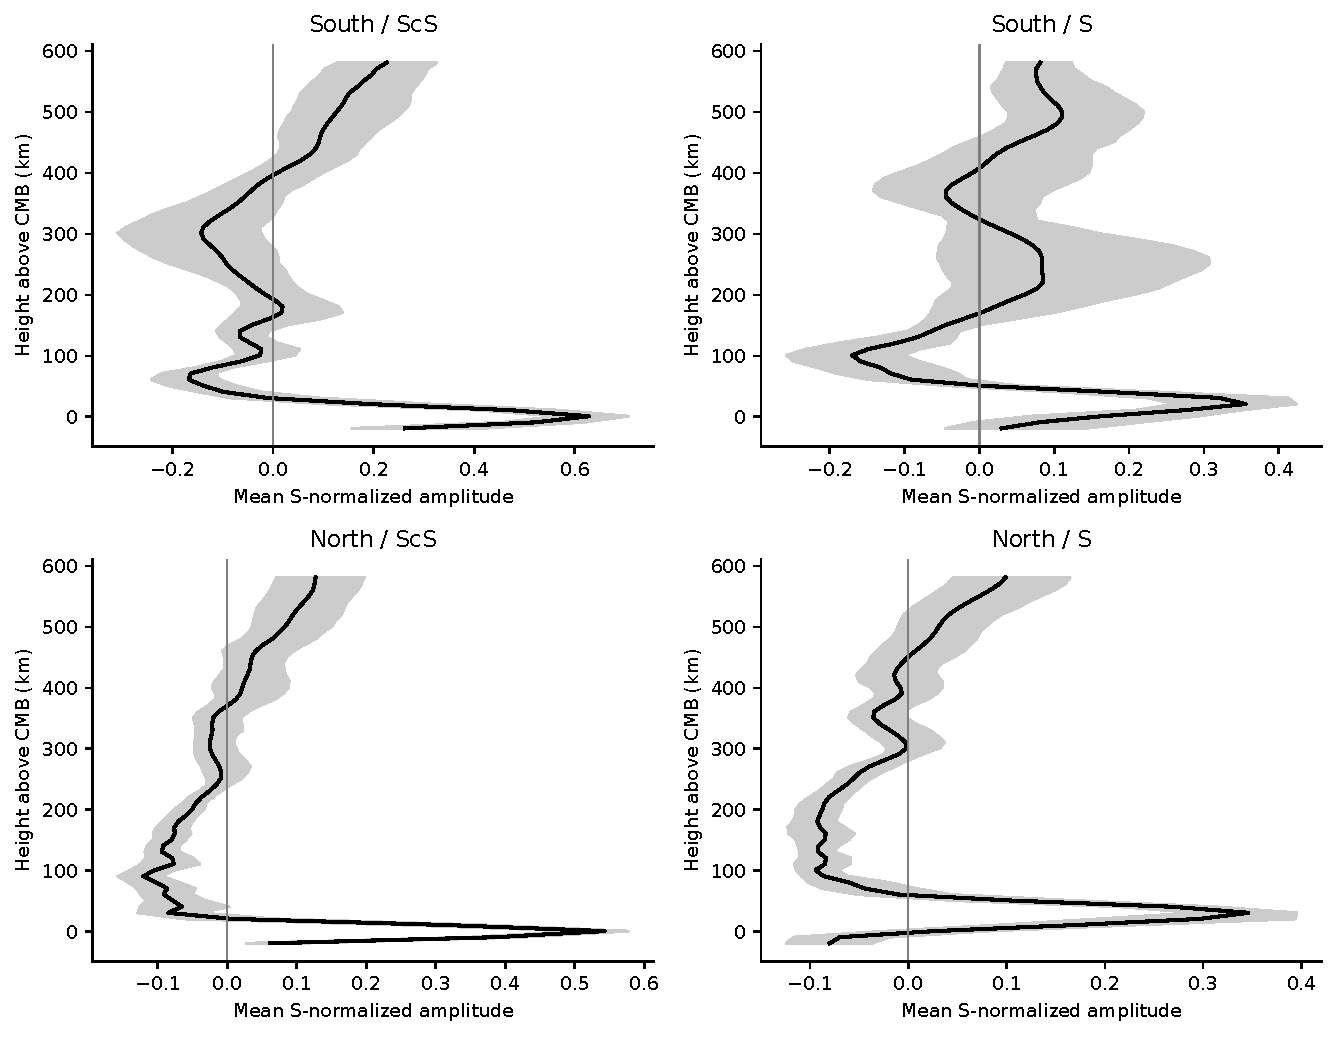
\includegraphics[width=.96\linewidth,height=.87\textheight,keepaspectratio]{figures/modern_same/supplement11.pdf}
\caption{modern\_same; independent supplementary figure 11 counterpart. Definitions, assumptions, and panel status are given in the panel record. All numerical values come from saved arrays.}\end{figure}
\begin{figure}[p]\centering
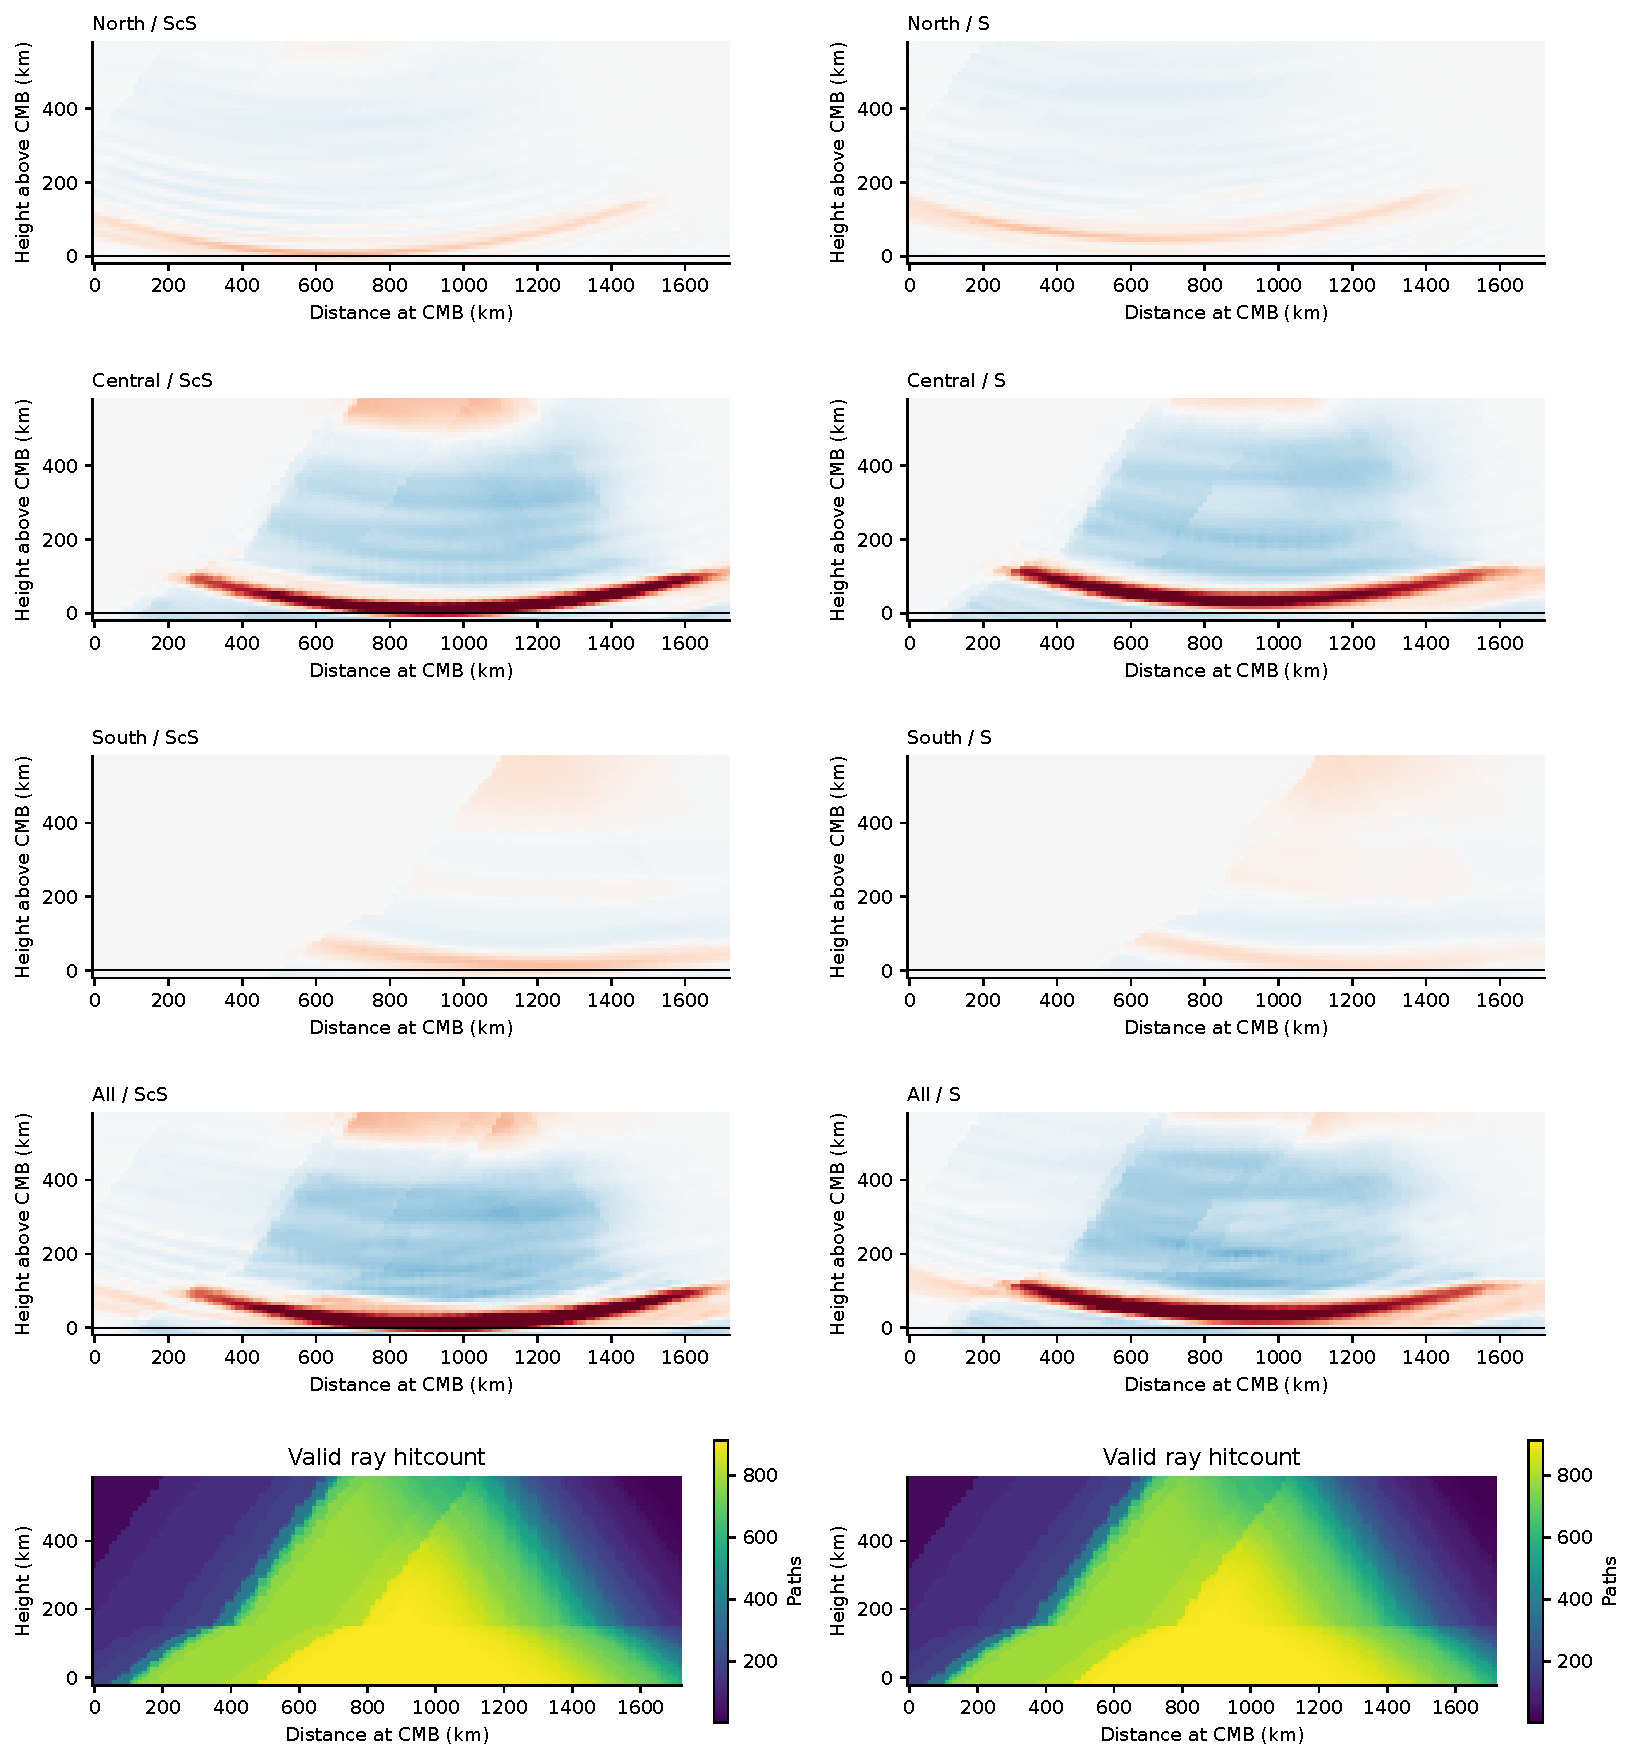
\includegraphics[width=.96\linewidth,height=.87\textheight,keepaspectratio]{figures/expanded/supplement2.pdf}
\caption{expanded; independent supplementary figure 2 counterpart. Definitions, assumptions, and panel status are given in the panel record. All numerical values come from saved arrays.}\end{figure}
\begin{figure}[p]\centering
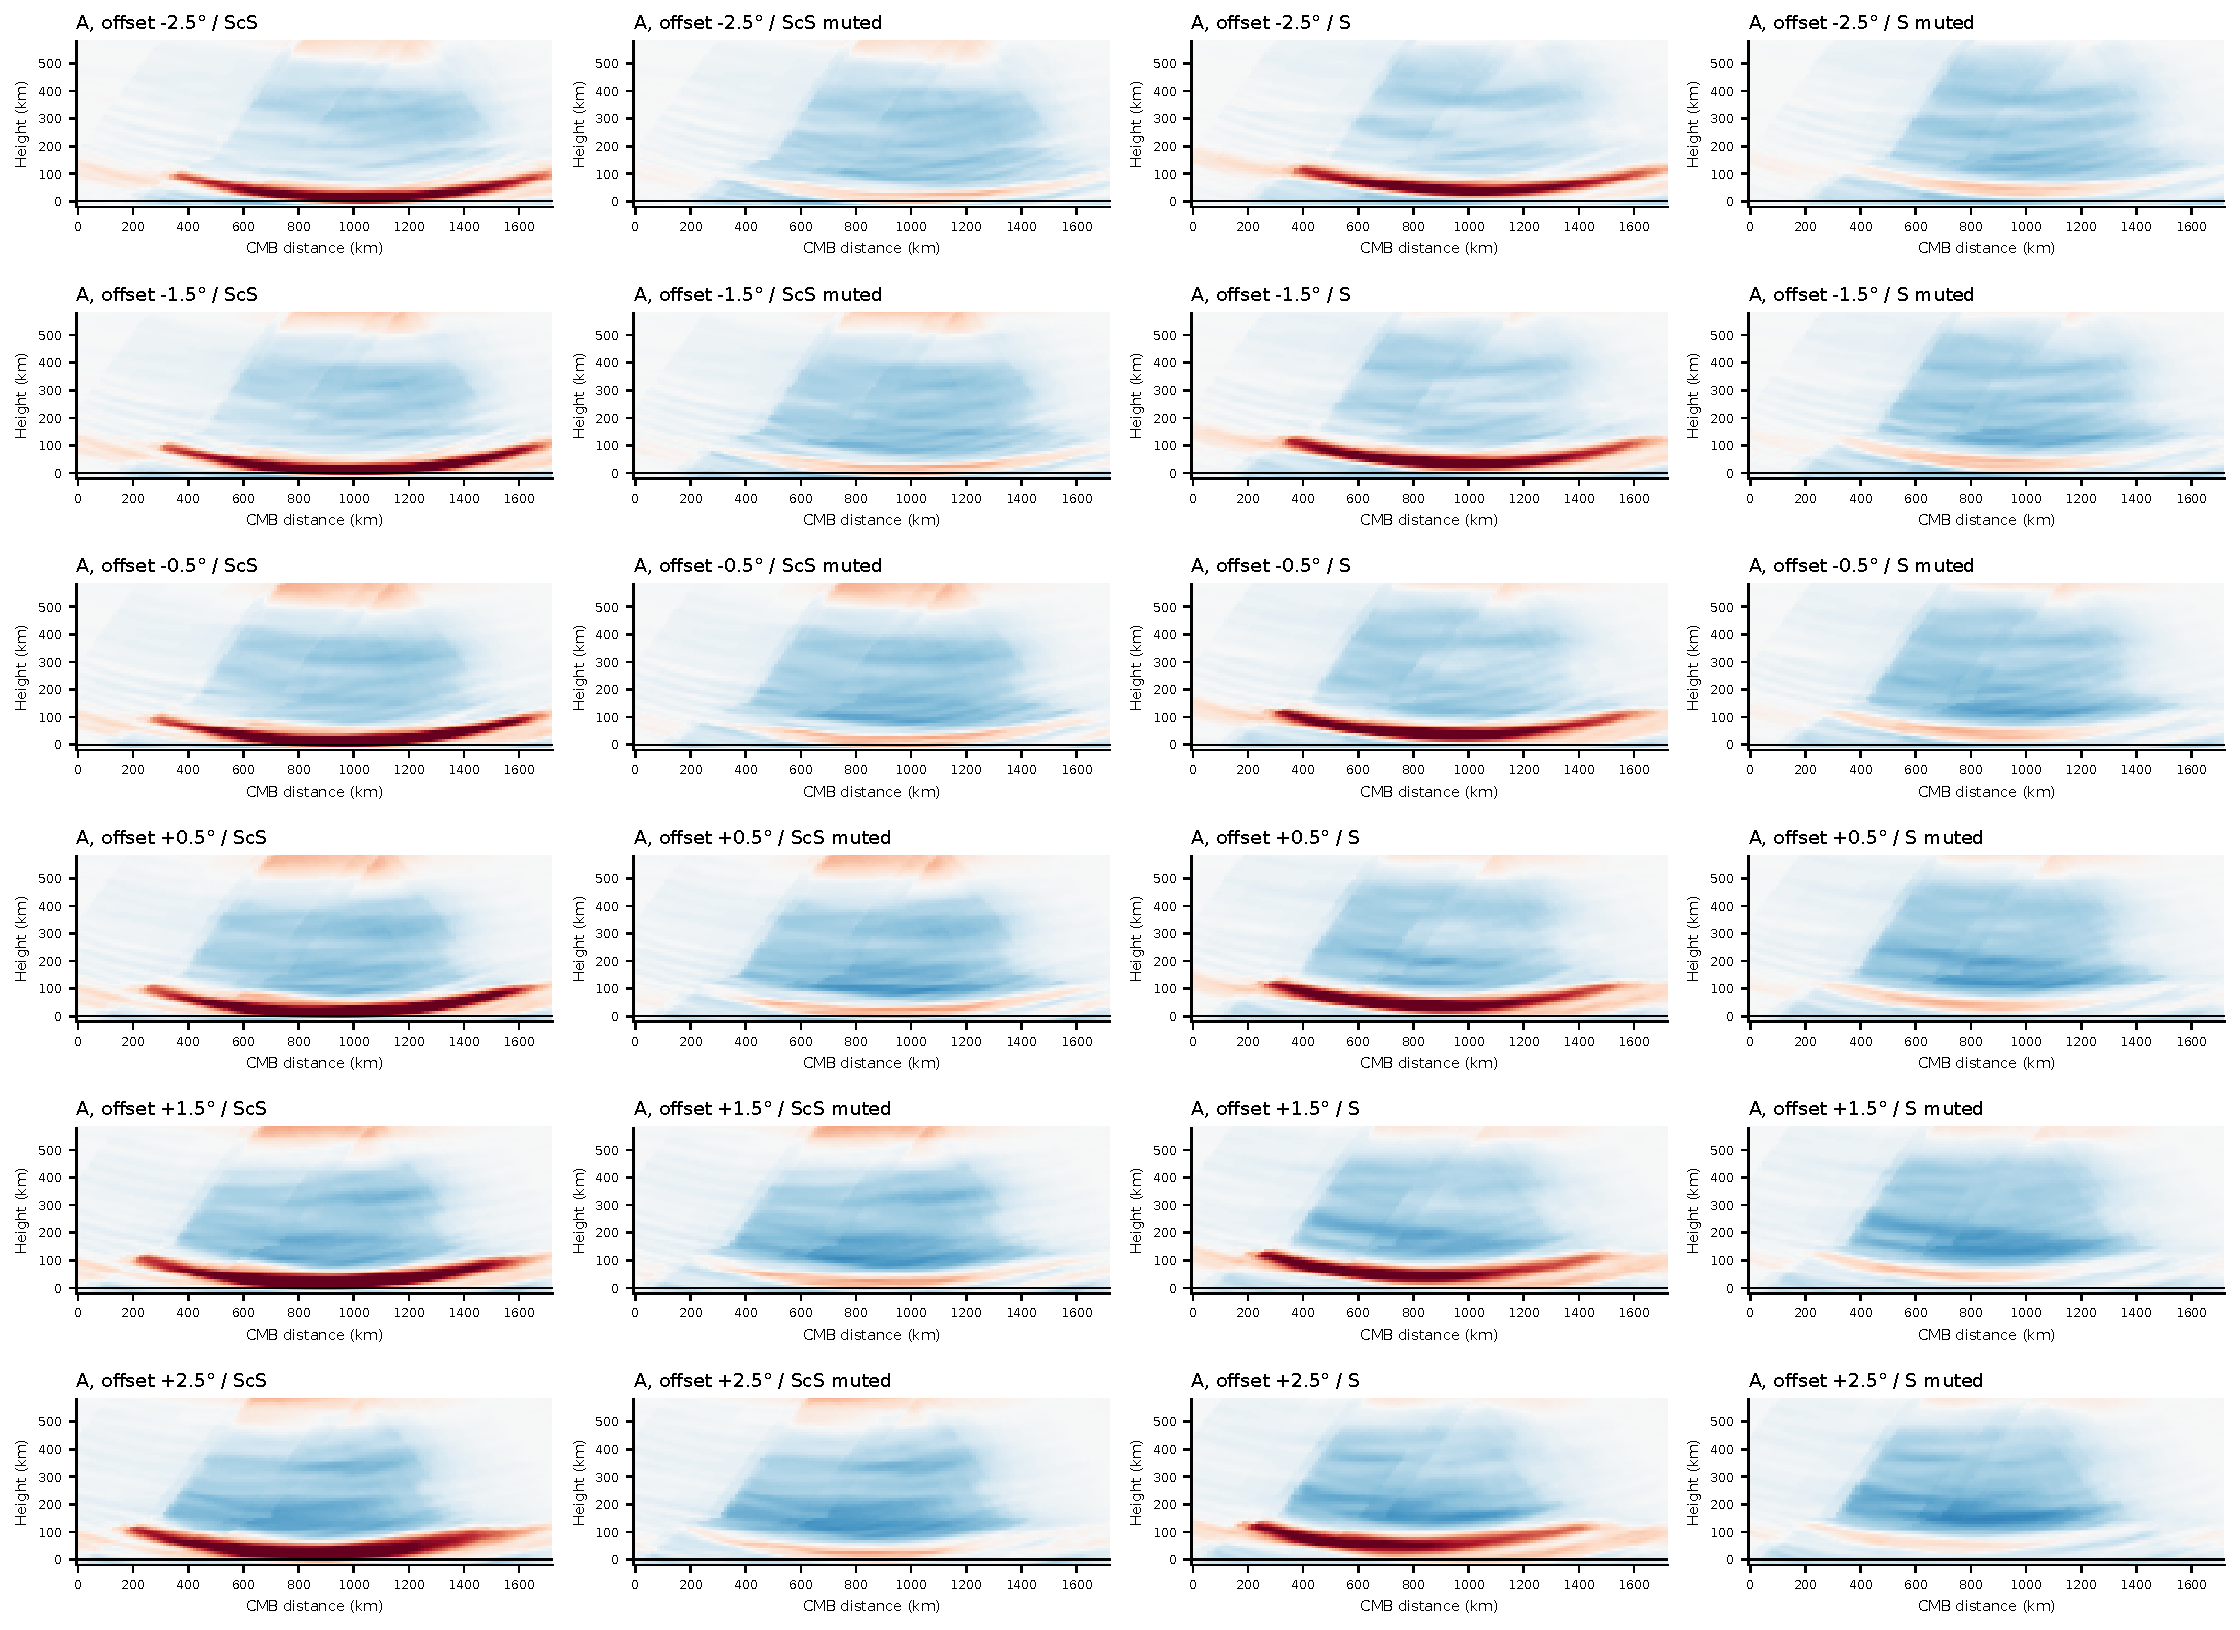
\includegraphics[width=.96\linewidth,height=.87\textheight,keepaspectratio]{figures/expanded/supplement3a.pdf}
\caption{expanded; independent supplementary figure 3a counterpart. Definitions, assumptions, and panel status are given in the panel record. All numerical values come from saved arrays.}\end{figure}
\begin{figure}[p]\centering
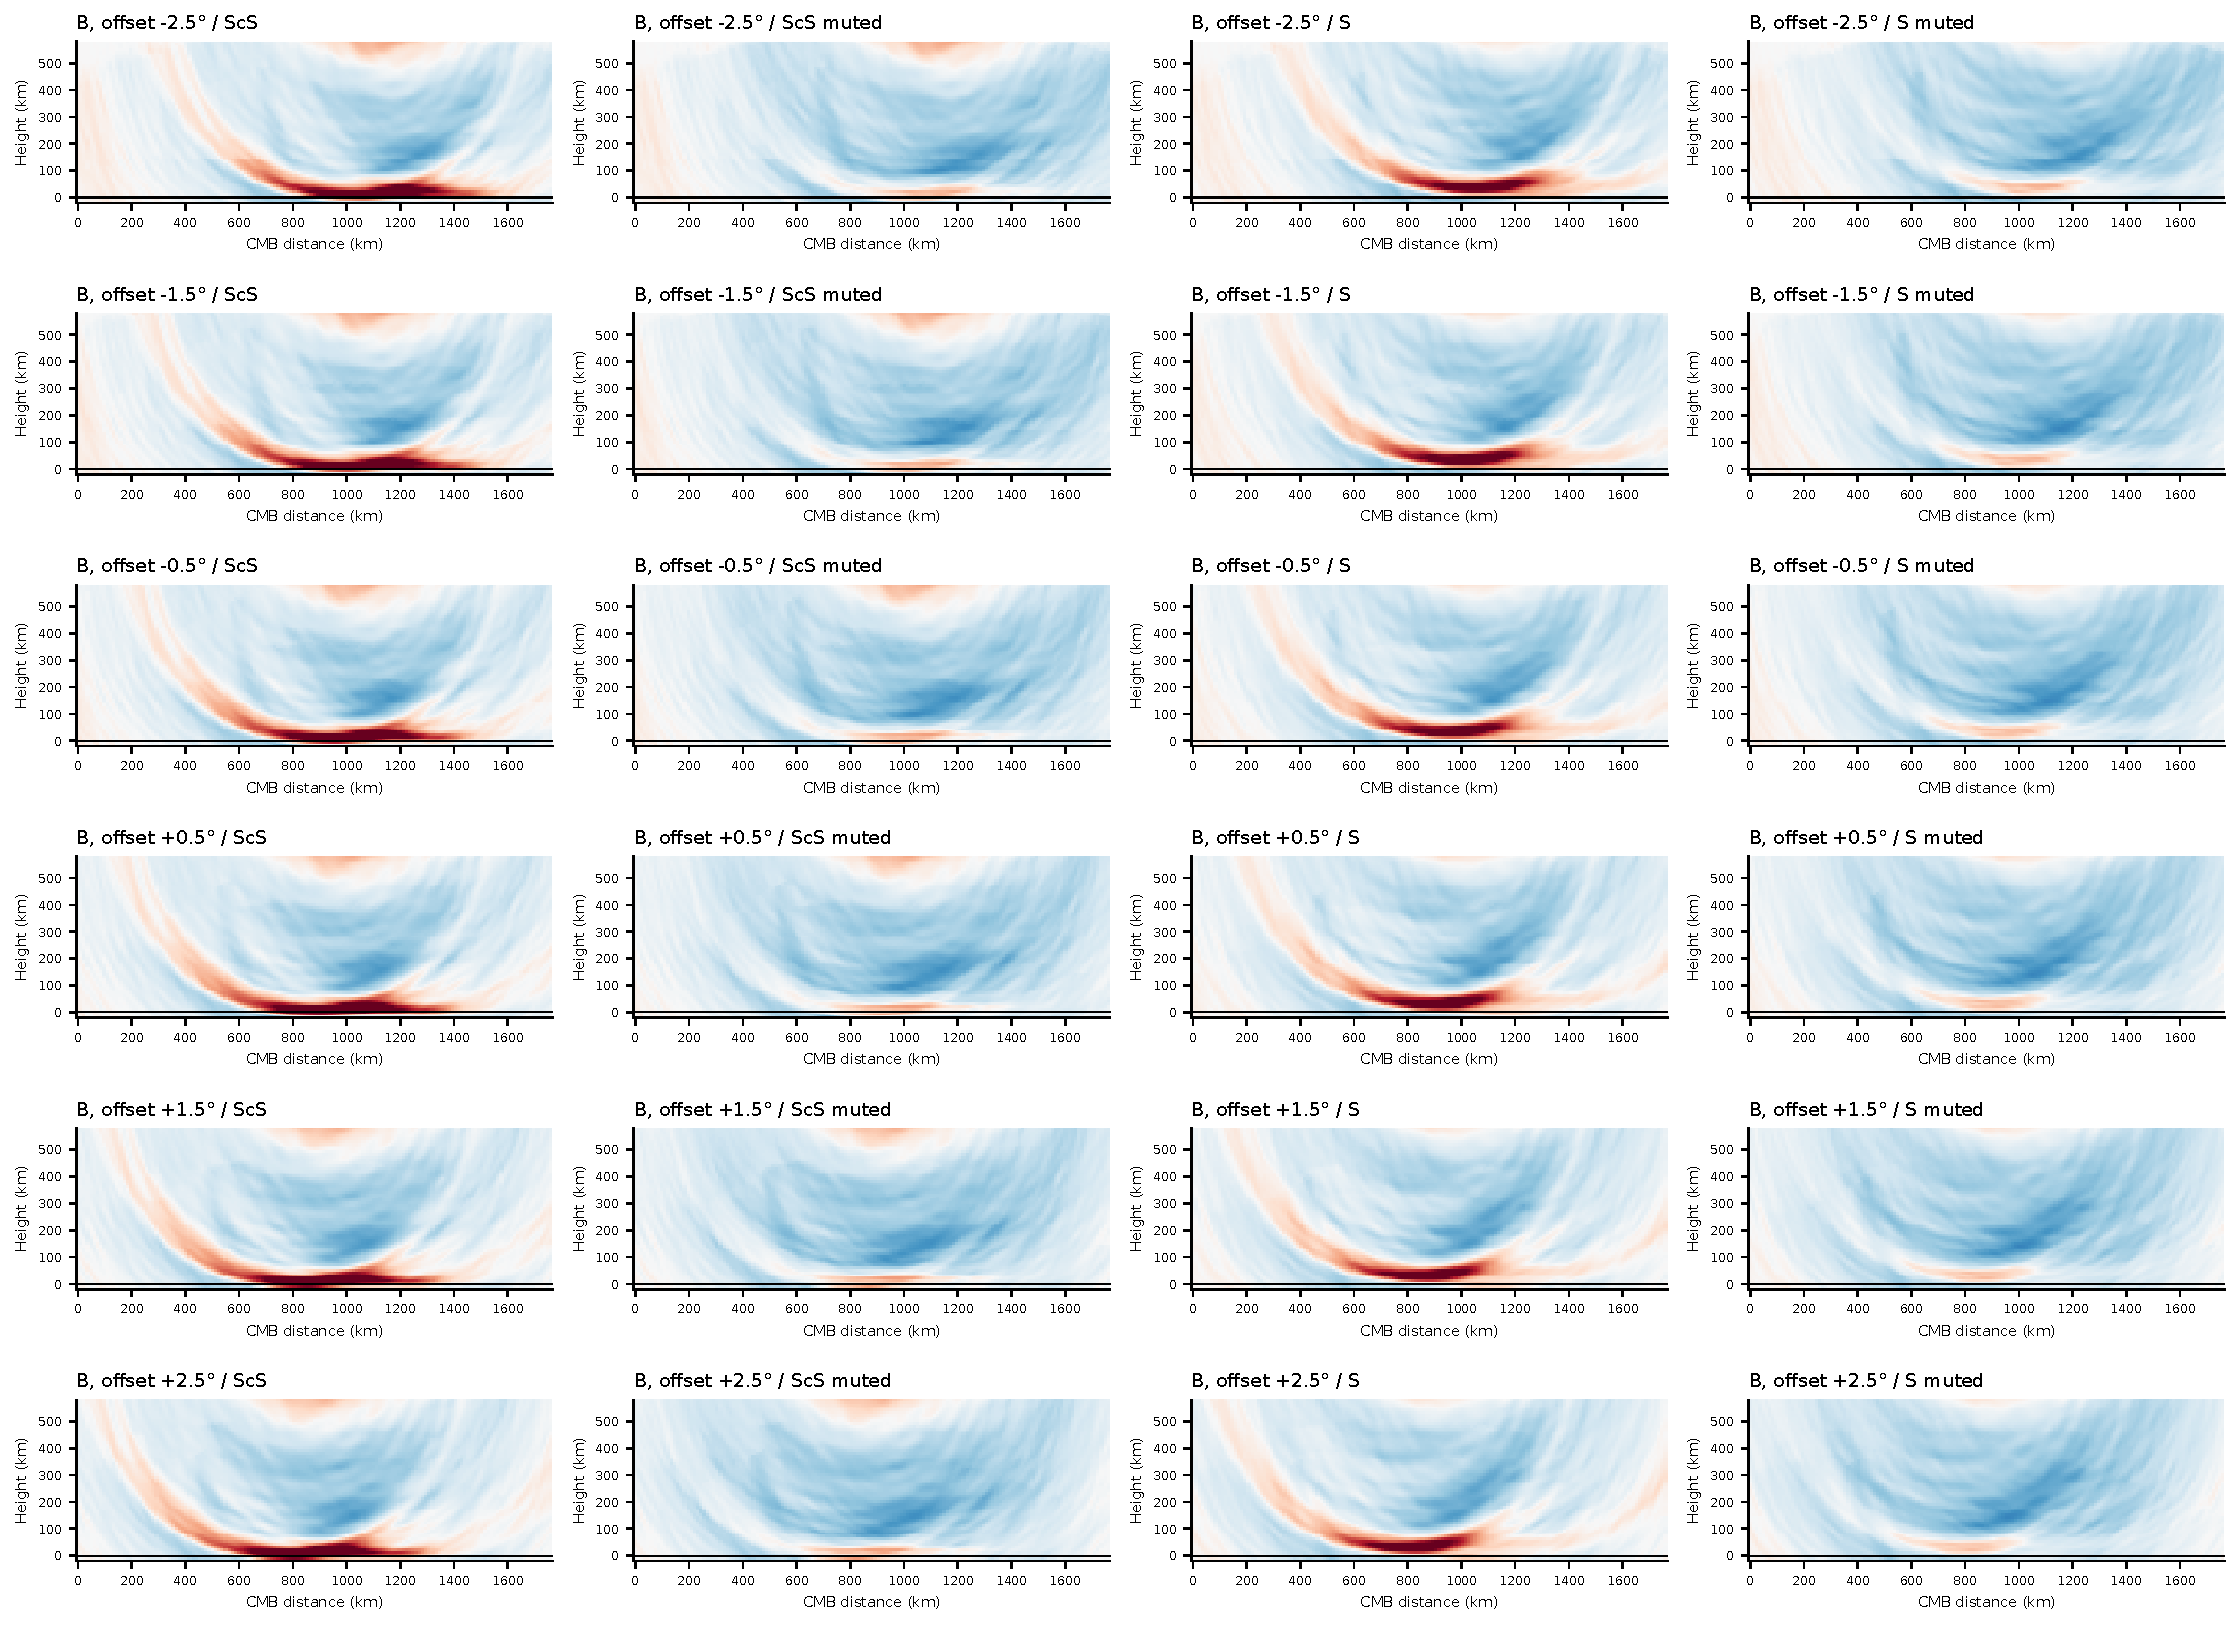
\includegraphics[width=.96\linewidth,height=.87\textheight,keepaspectratio]{figures/expanded/supplement3b.pdf}
\caption{expanded; independent supplementary figure 3b counterpart. Definitions, assumptions, and panel status are given in the panel record. All numerical values come from saved arrays.}\end{figure}
\begin{figure}[p]\centering
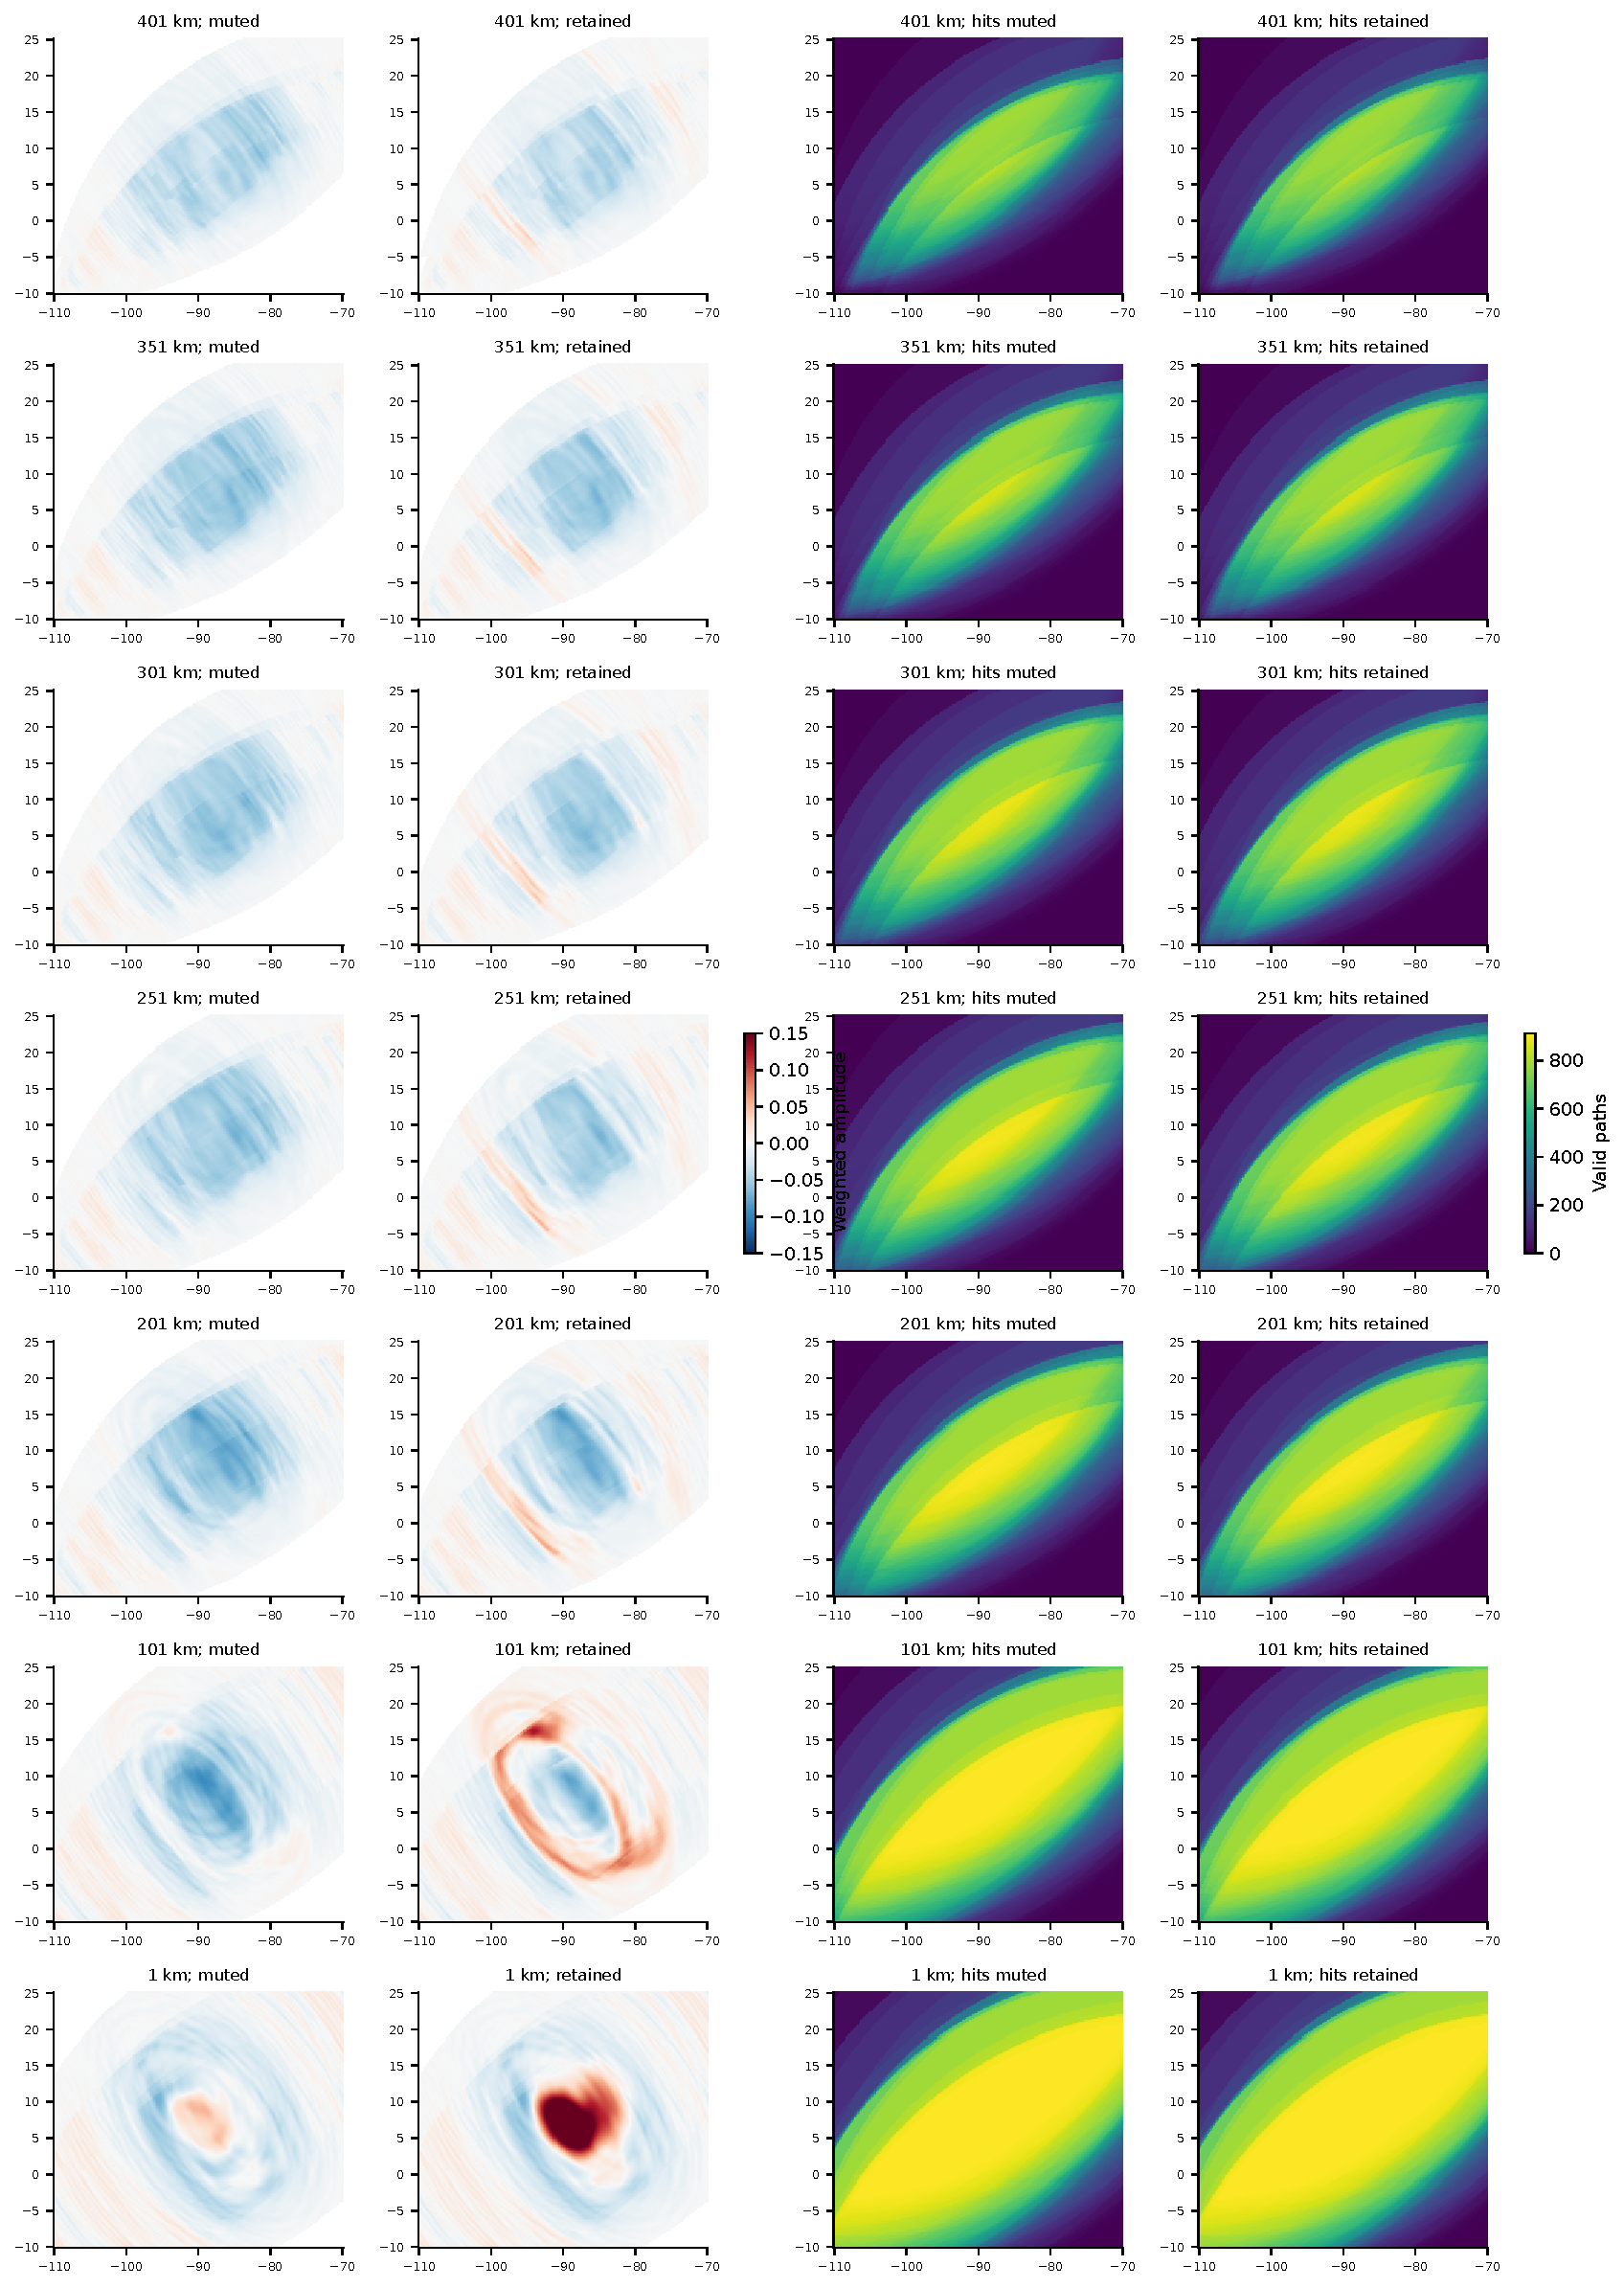
\includegraphics[width=.96\linewidth,height=.87\textheight,keepaspectratio]{figures/expanded/supplement5.pdf}
\caption{expanded; independent supplementary figure 5 counterpart. Definitions, assumptions, and panel status are given in the panel record. All numerical values come from saved arrays.}\end{figure}
\begin{figure}[p]\centering
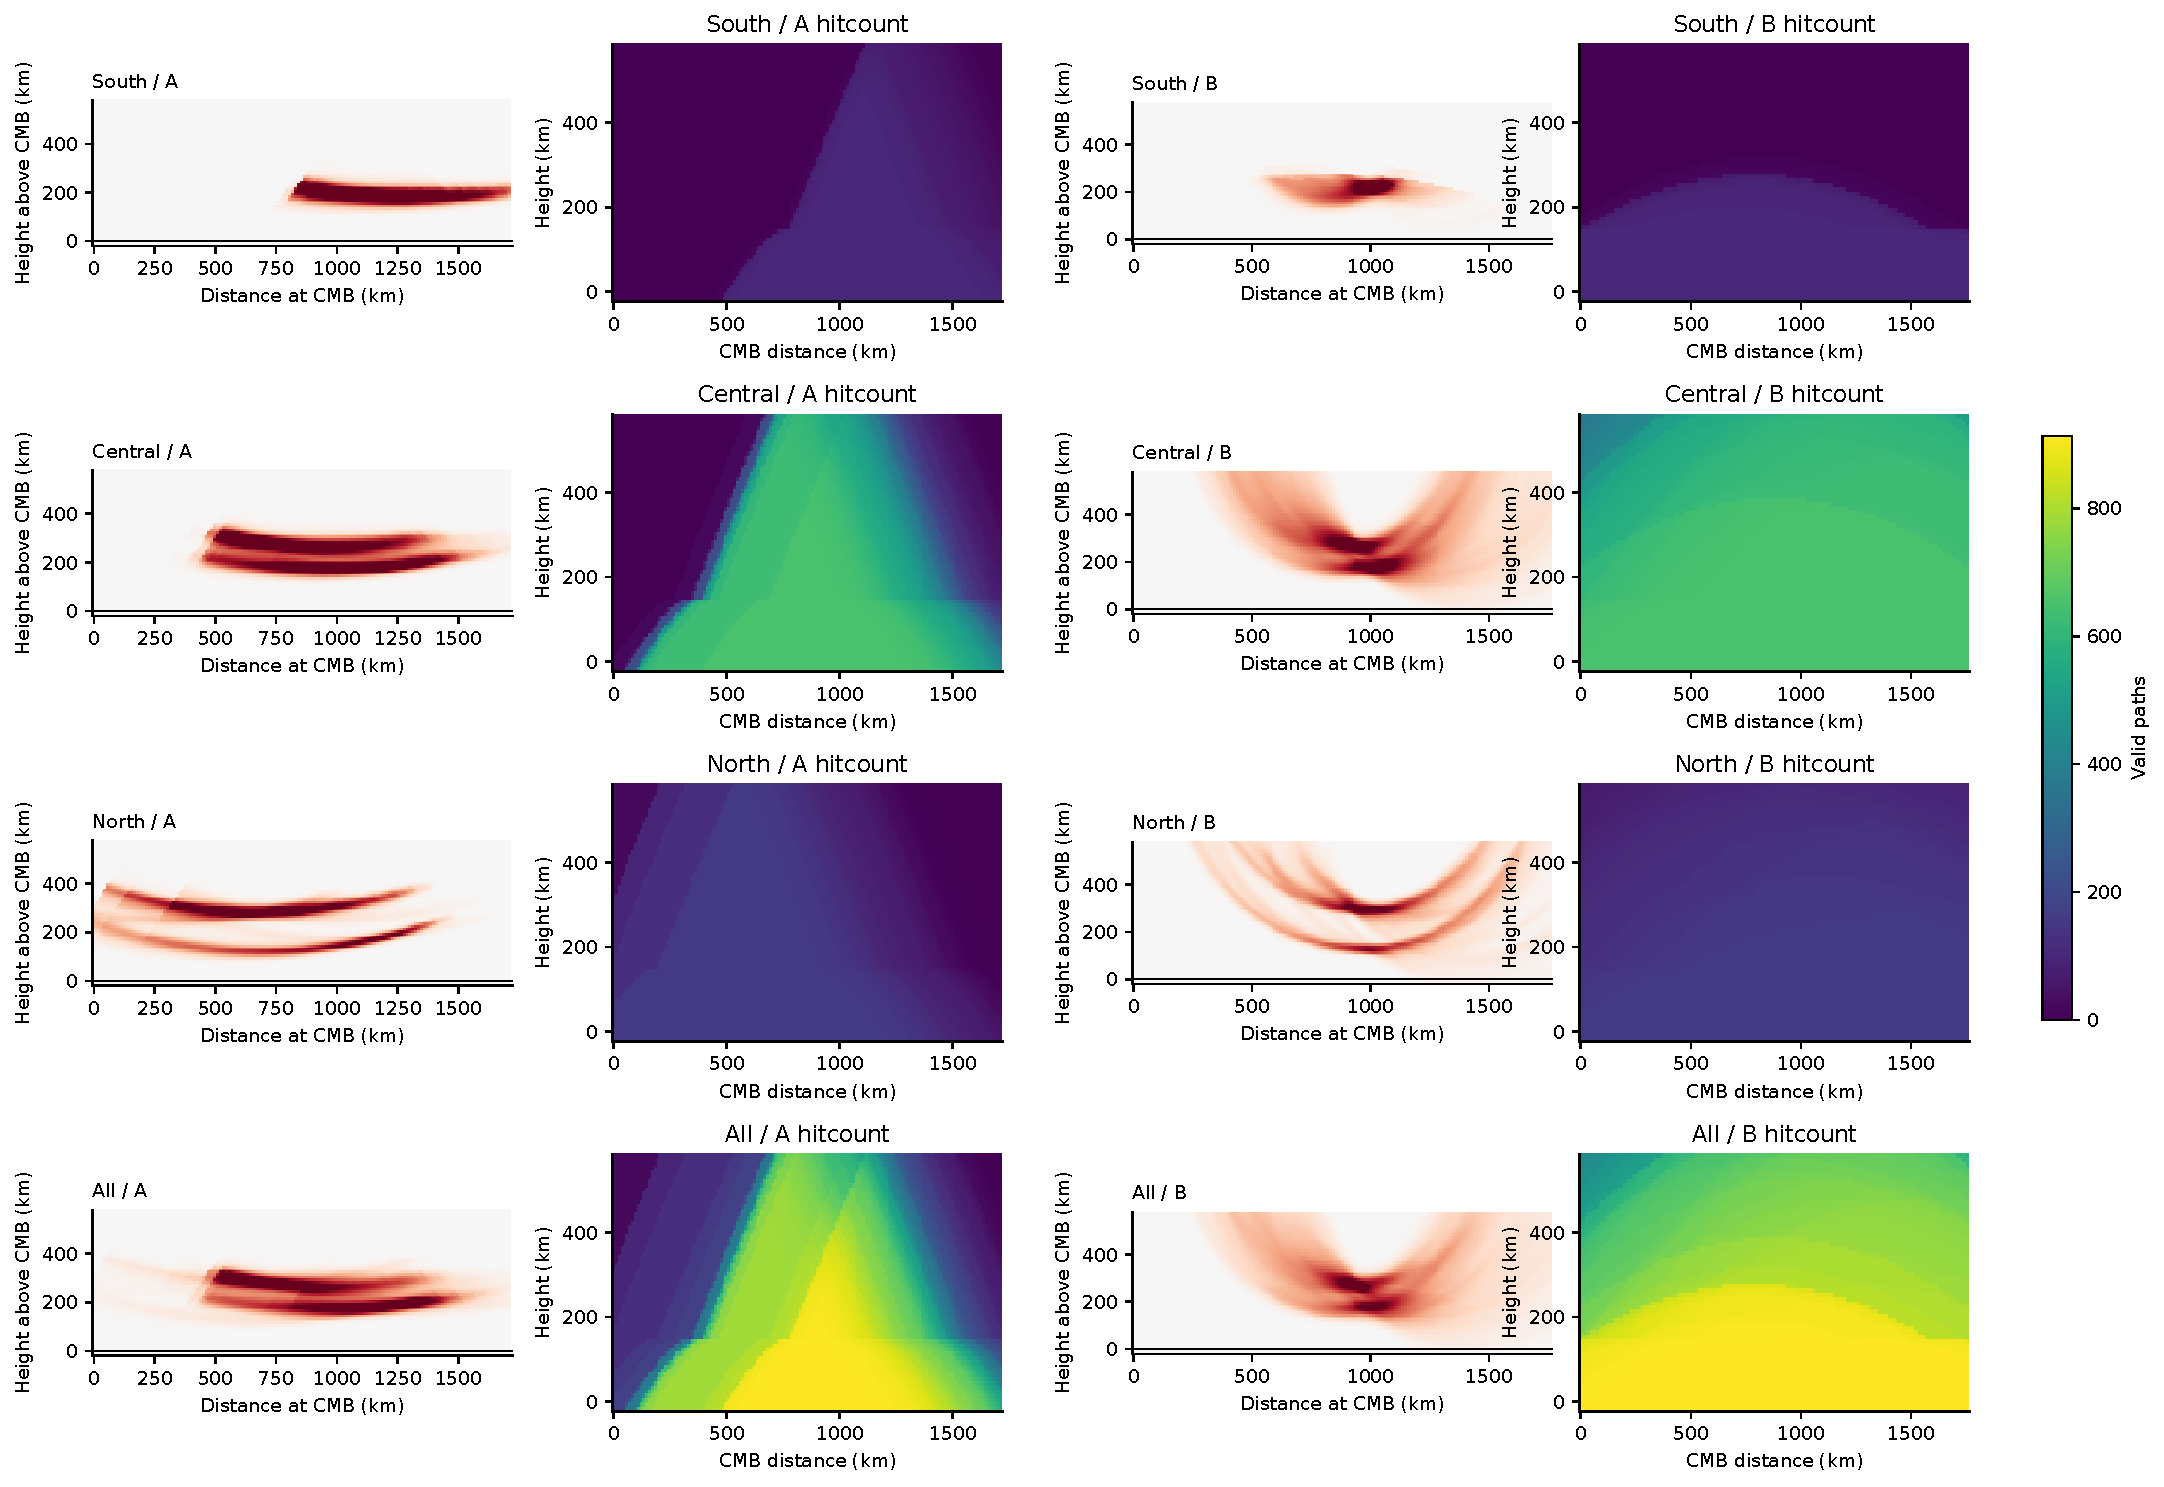
\includegraphics[width=.96\linewidth,height=.87\textheight,keepaspectratio]{figures/expanded/supplement6.pdf}
\caption{expanded; independent supplementary figure 6 counterpart. Definitions, assumptions, and panel status are given in the panel record. All numerical values come from saved arrays.}\end{figure}
\begin{figure}[p]\centering
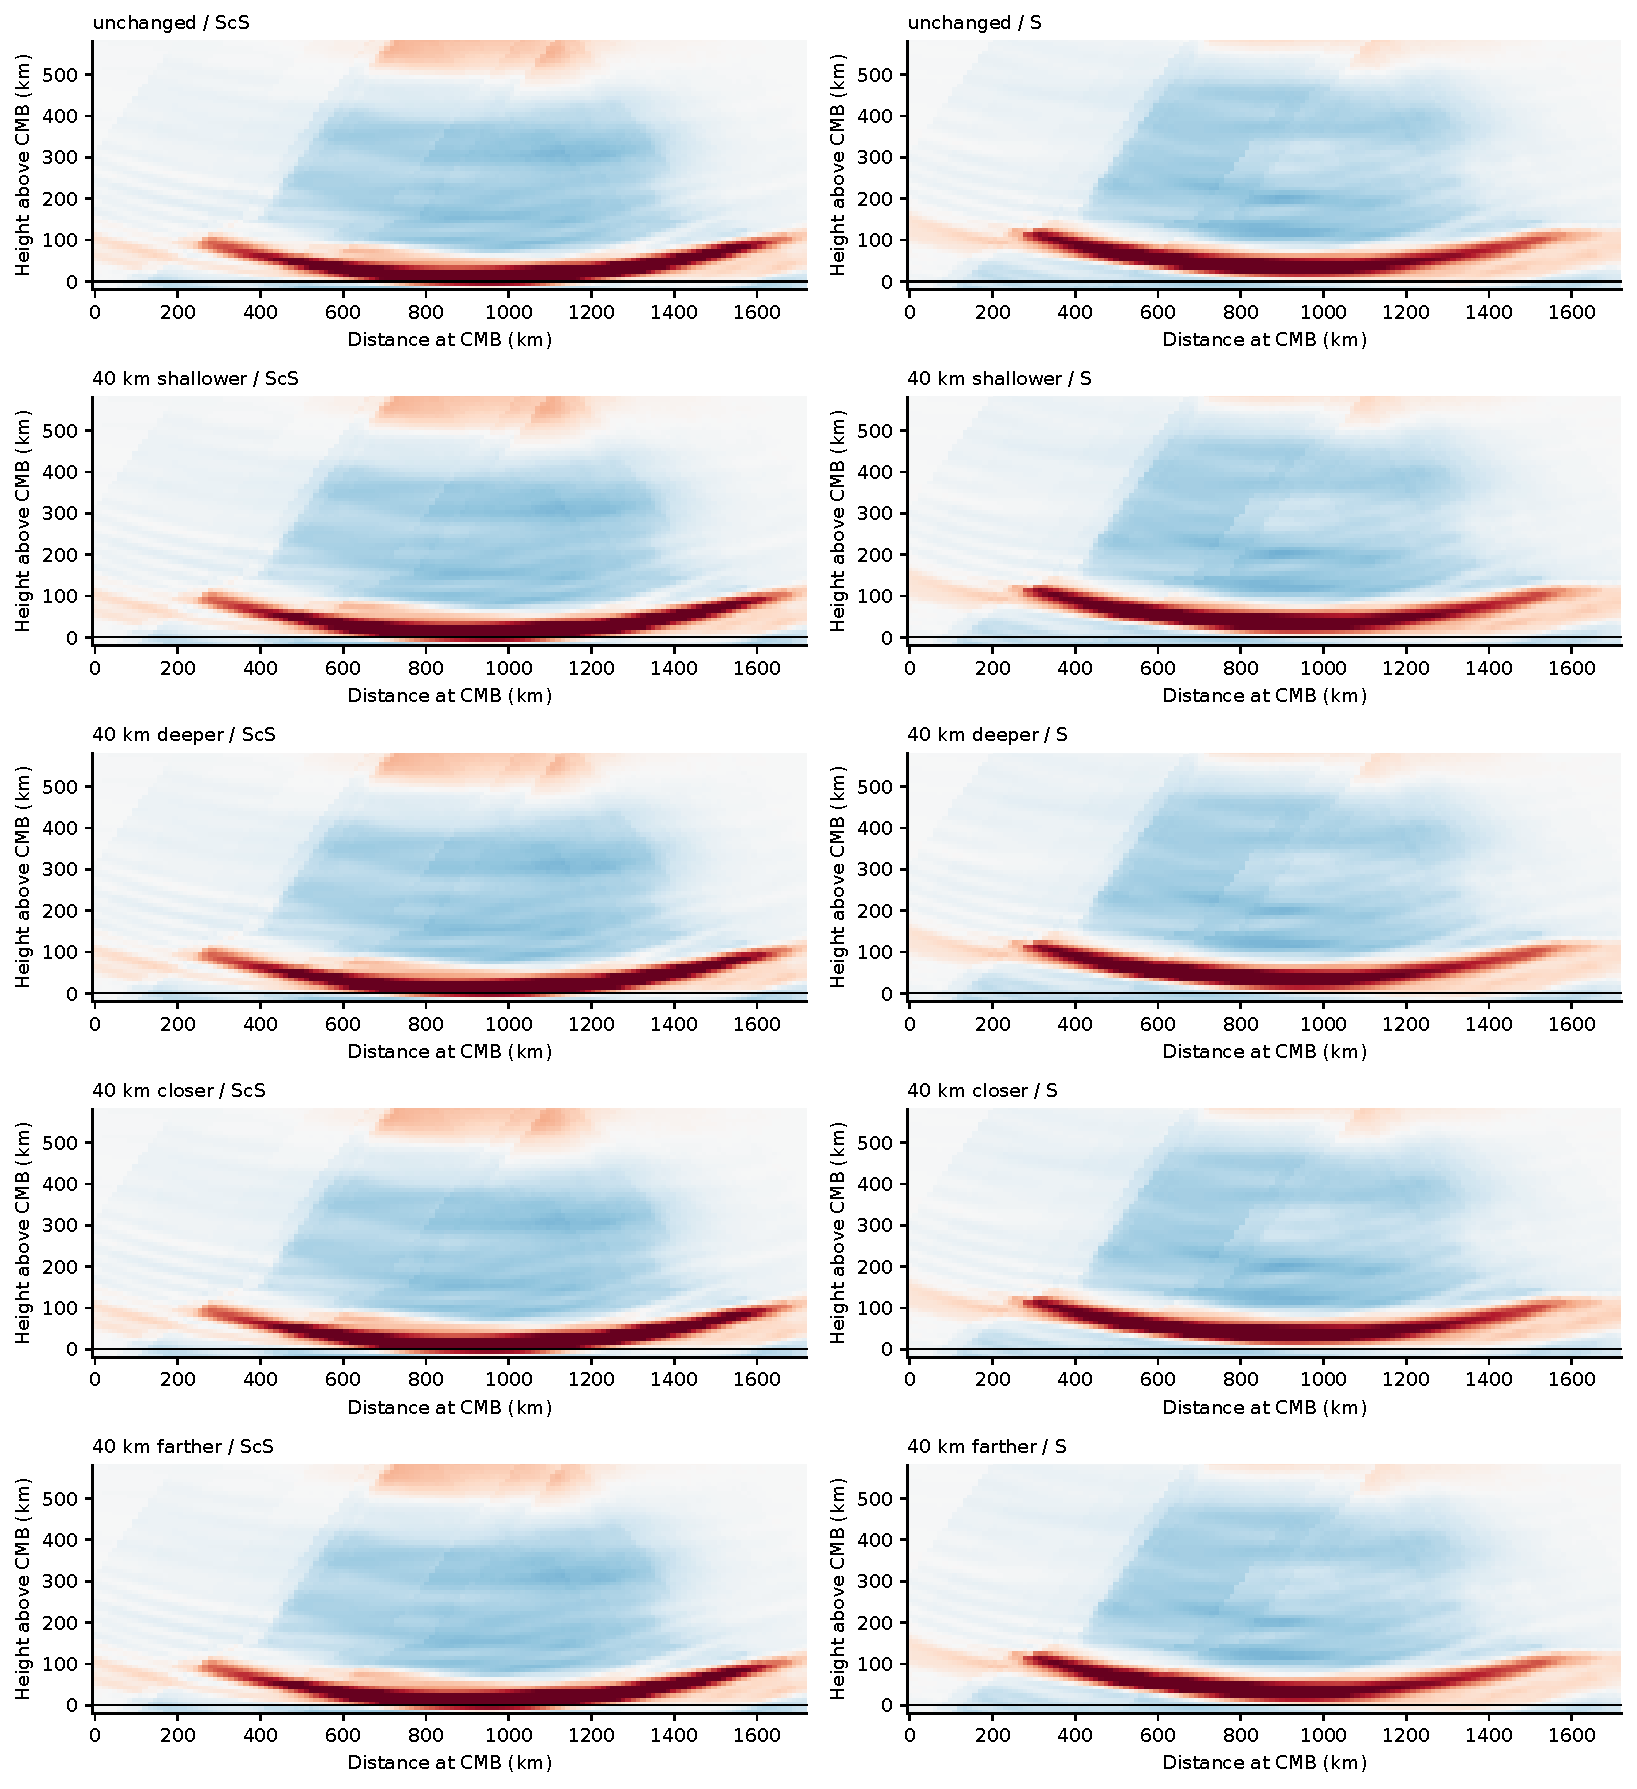
\includegraphics[width=.96\linewidth,height=.87\textheight,keepaspectratio]{figures/expanded/supplement10.pdf}
\caption{expanded; independent supplementary figure 10 counterpart. Definitions, assumptions, and panel status are given in the panel record. All numerical values come from saved arrays.}\end{figure}
\begin{figure}[p]\centering
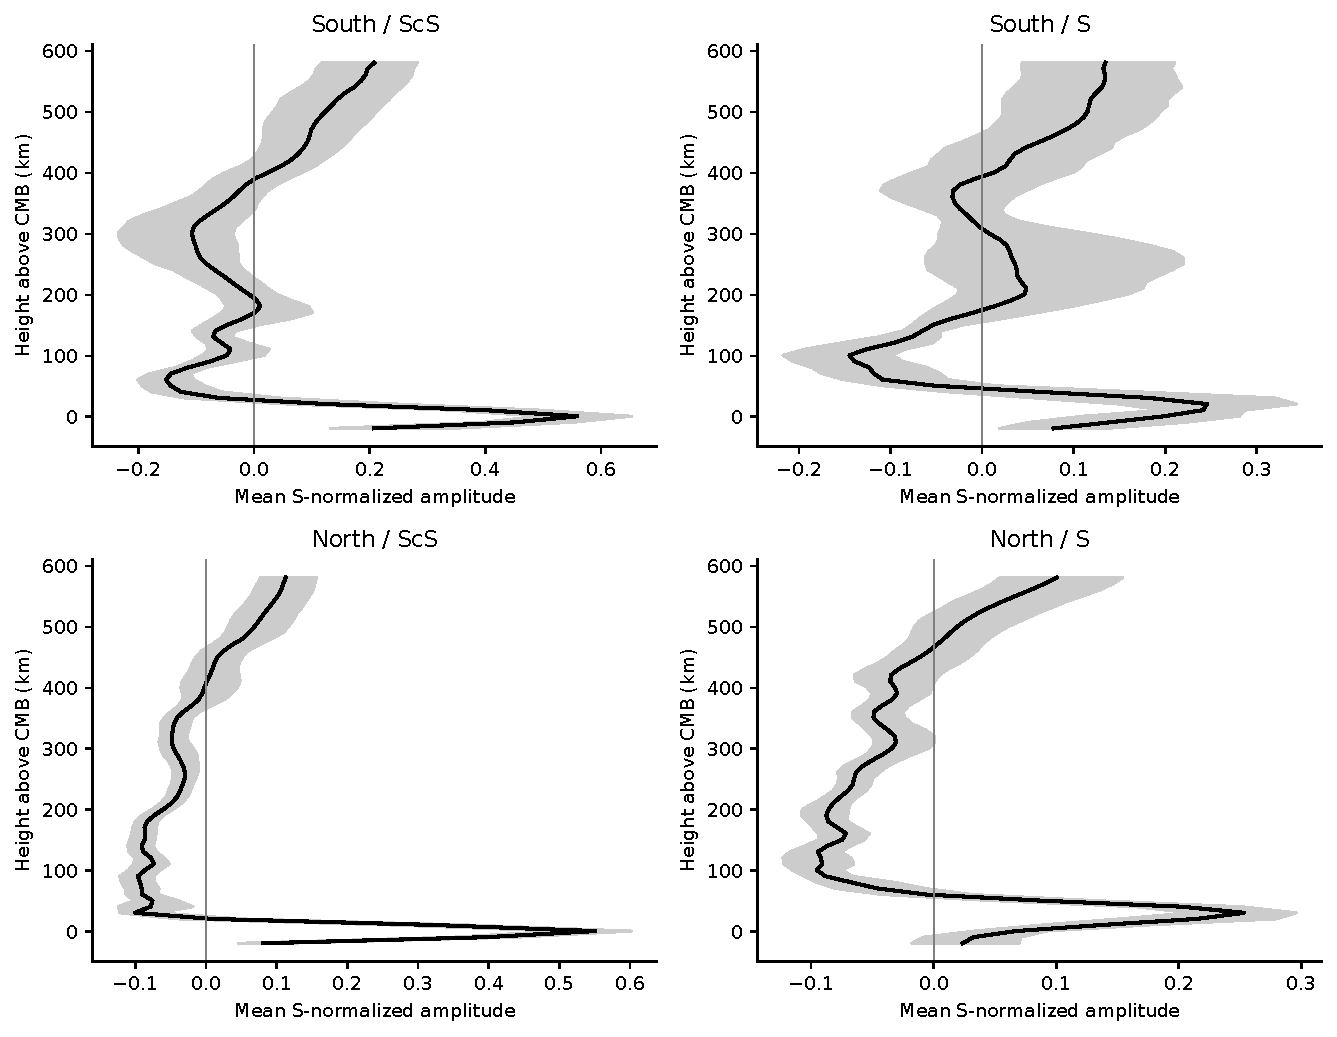
\includegraphics[width=.96\linewidth,height=.87\textheight,keepaspectratio]{figures/expanded/supplement11.pdf}
\caption{expanded; independent supplementary figure 11 counterpart. Definitions, assumptions, and panel status are given in the panel record. All numerical values come from saved arrays.}\end{figure}
\clearpage\section{Panel-by-panel provenance and status}
The complete machine-readable records are \texttt{report/panels.csv} and
\texttt{report/panels.json}. Every row gives its quantity, documentation,
parameters, data command, plot command, status, and limitation. The listing below
includes every identified main and supplementary subpanel. The same status applies
to each of the three generated dataset series unless a row explicitly names
a separate schematic or unavailable calculation. Point-source resolution and
source-location sensitivity are recomputed for each dataset geometry. In command strings,
\texttt{DATASET} means \texttt{historical}, \texttt{modern\_same}, or
\texttt{expanded}. Parameters are fixed in \texttt{config.json} and described
in the methods; no image-based tuning is used. ``Partially reproduced'' means
independently generated but incomplete in inputs, method, or comparison, not a
copied or digitized result. ``Not reproduced'' has no substituted numerical plot.

Command key (run from the project root):
\begin{center}\begin{tabular}{ll}
A & \texttt{python scripts/acquire.py}\\
  & \texttt{python scripts/process.py --workers 16}\\
M & \texttt{python scripts/migrate.py --dataset DATASET}\\
E & \texttt{python scripts/experiments.py --dataset DATASET}\\
V & \texttt{python scripts/validate.py --points --dataset DATASET}\\
L & \texttt{python scripts/sensitivity.py DATASET}\\
P & \texttt{python scripts/plot.py --dataset DATASET}\\
\end{tabular}\end{center}
 All E-only input-model and
ray examples can be generated with \texttt{--synthetics-only}. Rows sharing
a command still have separate entries in the accompanying complete CSV.
\small
\begin{longtable}{p{.23\linewidth}p{.25\linewidth}p{.19\linewidth}p{.22\linewidth}}
\toprule Panel & Quantity & Status & Data / plot commands\\\midrule\endhead
1 map & Event/station locations, ScS bounce points, profiles & partially reproduced & A, M / P \\
1 ray inset & S and ScS paths & partially reproduced & E / P \\
1 triplication inset & Sbc and Scd branch geometry & schematic redrawn & schematic / P \\
1 waveform inset & S, Scd+Sbc and ScS waveforms & partially reproduced & E / P \\
2a A & Signed migration amplitude, profile A; ScS retained & partially reproduced & A, M / P \\
2a B & Signed migration amplitude, profile B; ScS retained & partially reproduced & A, M / P \\
2b A & Signed migration amplitude, profile A; ScS censored & partially reproduced & A, M / P \\
2b B & Signed migration amplitude, profile B; ScS censored & partially reproduced & A, M / P \\
3 PREM & ScS-reference profile A in PREM & partially reproduced & A, M / P \\
3 UT & ScS-reference profile A in UT & not reproduced & unavailable / no substitute \\
3 UCB & ScS-reference profile A in UCB & not reproduced & unavailable / no substitute \\
3 CIT & ScS-reference profile A in CIT & not reproduced & unavailable / no substitute \\
4 upper & Folded slab and phase-boundary interpretation & schematic redrawn & schematic / P \\
4 lower & Profile A migration image & partially reproduced & A, M / P \\
S1 map & Geometry, mechanisms, Fresnel ellipses & partially reproduced & A, M / P \\
S2 ScS North & Clustered profile or contributing ray count & partially reproduced & A, M / P \\
S2 ScS Central & Clustered profile or contributing ray count & partially reproduced & A, M / P \\
S2 ScS South & Clustered profile or contributing ray count & partially reproduced & A, M / P \\
S2 ScS All & Clustered profile or contributing ray count & partially reproduced & A, M / P \\
S2 ScS hitcount & Clustered profile or contributing ray count & partially reproduced & A, M / P \\
S2 S North & Clustered profile or contributing ray count & partially reproduced & A, M / P \\
S2 S Central & Clustered profile or contributing ray count & partially reproduced & A, M / P \\
S2 S South & Clustered profile or contributing ray count & partially reproduced & A, M / P \\
S2 S All & Clustered profile or contributing ray count & partially reproduced & A, M / P \\
S2 S hitcount & Clustered profile or contributing ray count & partially reproduced & A, M / P \\
S3a A ScS retained & Parallel vertical migration section & partially reproduced & A, M / P \\
S3a A ScS censored & Parallel vertical migration section & partially reproduced & A, M / P \\
S3a A S retained & Parallel vertical migration section & partially reproduced & A, M / P \\
S3a A S censored & Parallel vertical migration section & partially reproduced & A, M / P \\
S3a B ScS retained & Parallel vertical migration section & partially reproduced & A, M / P \\
S3a B ScS censored & Parallel vertical migration section & partially reproduced & A, M / P \\
S3a B S retained & Parallel vertical migration section & partially reproduced & A, M / P \\
S3a B S censored & Parallel vertical migration section & partially reproduced & A, M / P \\
S3a C ScS retained & Parallel vertical migration section & partially reproduced & A, M / P \\
S3a C ScS censored & Parallel vertical migration section & partially reproduced & A, M / P \\
S3a C S retained & Parallel vertical migration section & partially reproduced & A, M / P \\
S3a C S censored & Parallel vertical migration section & partially reproduced & A, M / P \\
S3a D ScS retained & Parallel vertical migration section & partially reproduced & A, M / P \\
S3a D ScS censored & Parallel vertical migration section & partially reproduced & A, M / P \\
S3a D S retained & Parallel vertical migration section & partially reproduced & A, M / P \\
S3a D S censored & Parallel vertical migration section & partially reproduced & A, M / P \\
S3a E ScS retained & Parallel vertical migration section & partially reproduced & A, M / P \\
S3a E ScS censored & Parallel vertical migration section & partially reproduced & A, M / P \\
S3a E S retained & Parallel vertical migration section & partially reproduced & A, M / P \\
S3a E S censored & Parallel vertical migration section & partially reproduced & A, M / P \\
S3a F ScS retained & Parallel vertical migration section & partially reproduced & A, M / P \\
S3a F ScS censored & Parallel vertical migration section & partially reproduced & A, M / P \\
S3a F S retained & Parallel vertical migration section & partially reproduced & A, M / P \\
S3a F S censored & Parallel vertical migration section & partially reproduced & A, M / P \\
S3b U ScS retained & Parallel vertical migration section & partially reproduced & A, M / P \\
S3b U ScS censored & Parallel vertical migration section & partially reproduced & A, M / P \\
S3b U S retained & Parallel vertical migration section & partially reproduced & A, M / P \\
S3b U S censored & Parallel vertical migration section & partially reproduced & A, M / P \\
S3b V ScS retained & Parallel vertical migration section & partially reproduced & A, M / P \\
S3b V ScS censored & Parallel vertical migration section & partially reproduced & A, M / P \\
S3b V S retained & Parallel vertical migration section & partially reproduced & A, M / P \\
S3b V S censored & Parallel vertical migration section & partially reproduced & A, M / P \\
S3b W ScS retained & Parallel vertical migration section & partially reproduced & A, M / P \\
S3b W ScS censored & Parallel vertical migration section & partially reproduced & A, M / P \\
S3b W S retained & Parallel vertical migration section & partially reproduced & A, M / P \\
S3b W S censored & Parallel vertical migration section & partially reproduced & A, M / P \\
S3b X ScS retained & Parallel vertical migration section & partially reproduced & A, M / P \\
S3b X ScS censored & Parallel vertical migration section & partially reproduced & A, M / P \\
S3b X S retained & Parallel vertical migration section & partially reproduced & A, M / P \\
S3b X S censored & Parallel vertical migration section & partially reproduced & A, M / P \\
S3b Y ScS retained & Parallel vertical migration section & partially reproduced & A, M / P \\
S3b Y ScS censored & Parallel vertical migration section & partially reproduced & A, M / P \\
S3b Y S retained & Parallel vertical migration section & partially reproduced & A, M / P \\
S3b Y S censored & Parallel vertical migration section & partially reproduced & A, M / P \\
S3b Z ScS retained & Parallel vertical migration section & partially reproduced & A, M / P \\
S3b Z ScS censored & Parallel vertical migration section & partially reproduced & A, M / P \\
S3b Z S retained & Parallel vertical migration section & partially reproduced & A, M / P \\
S3b Z S censored & Parallel vertical migration section & partially reproduced & A, M / P \\
S4a A PREM & Velocity-model sensitivity: ScS retained & partially reproduced & A, M / P \\
S4a A UT & Velocity-model sensitivity: ScS retained & not reproduced & unavailable / no substitute \\
S4a A UCB & Velocity-model sensitivity: ScS retained & not reproduced & unavailable / no substitute \\
S4a A CIT & Velocity-model sensitivity: ScS retained & not reproduced & unavailable / no substitute \\
S4a B PREM & Velocity-model sensitivity: ScS retained & partially reproduced & A, M / P \\
S4a B UT & Velocity-model sensitivity: ScS retained & not reproduced & unavailable / no substitute \\
S4a B UCB & Velocity-model sensitivity: ScS retained & not reproduced & unavailable / no substitute \\
S4a B CIT & Velocity-model sensitivity: ScS retained & not reproduced & unavailable / no substitute \\
S4a C PREM & Velocity-model sensitivity: ScS retained & partially reproduced & A, M / P \\
S4a C UT & Velocity-model sensitivity: ScS retained & not reproduced & unavailable / no substitute \\
S4a C UCB & Velocity-model sensitivity: ScS retained & not reproduced & unavailable / no substitute \\
S4a C CIT & Velocity-model sensitivity: ScS retained & not reproduced & unavailable / no substitute \\
S4a D PREM & Velocity-model sensitivity: ScS retained & partially reproduced & A, M / P \\
S4a D UT & Velocity-model sensitivity: ScS retained & not reproduced & unavailable / no substitute \\
S4a D UCB & Velocity-model sensitivity: ScS retained & not reproduced & unavailable / no substitute \\
S4a D CIT & Velocity-model sensitivity: ScS retained & not reproduced & unavailable / no substitute \\
S4a E PREM & Velocity-model sensitivity: ScS retained & partially reproduced & A, M / P \\
S4a E UT & Velocity-model sensitivity: ScS retained & not reproduced & unavailable / no substitute \\
S4a E UCB & Velocity-model sensitivity: ScS retained & not reproduced & unavailable / no substitute \\
S4a E CIT & Velocity-model sensitivity: ScS retained & not reproduced & unavailable / no substitute \\
S4a F PREM & Velocity-model sensitivity: ScS retained & partially reproduced & A, M / P \\
S4a F UT & Velocity-model sensitivity: ScS retained & not reproduced & unavailable / no substitute \\
S4a F UCB & Velocity-model sensitivity: ScS retained & not reproduced & unavailable / no substitute \\
S4a F CIT & Velocity-model sensitivity: ScS retained & not reproduced & unavailable / no substitute \\
S4b A PREM & Velocity-model sensitivity: ScS censored & partially reproduced & A, M / P \\
S4b A UT & Velocity-model sensitivity: ScS censored & not reproduced & unavailable / no substitute \\
S4b A UCB & Velocity-model sensitivity: ScS censored & not reproduced & unavailable / no substitute \\
S4b A CIT & Velocity-model sensitivity: ScS censored & not reproduced & unavailable / no substitute \\
S4b B PREM & Velocity-model sensitivity: ScS censored & partially reproduced & A, M / P \\
S4b B UT & Velocity-model sensitivity: ScS censored & not reproduced & unavailable / no substitute \\
S4b B UCB & Velocity-model sensitivity: ScS censored & not reproduced & unavailable / no substitute \\
S4b B CIT & Velocity-model sensitivity: ScS censored & not reproduced & unavailable / no substitute \\
S4b C PREM & Velocity-model sensitivity: ScS censored & partially reproduced & A, M / P \\
S4b C UT & Velocity-model sensitivity: ScS censored & not reproduced & unavailable / no substitute \\
S4b C UCB & Velocity-model sensitivity: ScS censored & not reproduced & unavailable / no substitute \\
S4b C CIT & Velocity-model sensitivity: ScS censored & not reproduced & unavailable / no substitute \\
S4b D PREM & Velocity-model sensitivity: ScS censored & partially reproduced & A, M / P \\
S4b D UT & Velocity-model sensitivity: ScS censored & not reproduced & unavailable / no substitute \\
S4b D UCB & Velocity-model sensitivity: ScS censored & not reproduced & unavailable / no substitute \\
S4b D CIT & Velocity-model sensitivity: ScS censored & not reproduced & unavailable / no substitute \\
S4b E PREM & Velocity-model sensitivity: ScS censored & partially reproduced & A, M / P \\
S4b E UT & Velocity-model sensitivity: ScS censored & not reproduced & unavailable / no substitute \\
S4b E UCB & Velocity-model sensitivity: ScS censored & not reproduced & unavailable / no substitute \\
S4b E CIT & Velocity-model sensitivity: ScS censored & not reproduced & unavailable / no substitute \\
S4b F PREM & Velocity-model sensitivity: ScS censored & partially reproduced & A, M / P \\
S4b F UT & Velocity-model sensitivity: ScS censored & not reproduced & unavailable / no substitute \\
S4b F UCB & Velocity-model sensitivity: ScS censored & not reproduced & unavailable / no substitute \\
S4b F CIT & Velocity-model sensitivity: ScS censored & not reproduced & unavailable / no substitute \\
S4c A PREM & Velocity-model sensitivity: S reference, ScS retained & partially reproduced & A, M / P \\
S4c A UT & Velocity-model sensitivity: S reference, ScS retained & not reproduced & unavailable / no substitute \\
S4c A UCB & Velocity-model sensitivity: S reference, ScS retained & not reproduced & unavailable / no substitute \\
S4c A CIT & Velocity-model sensitivity: S reference, ScS retained & not reproduced & unavailable / no substitute \\
S4c B PREM & Velocity-model sensitivity: S reference, ScS retained & partially reproduced & A, M / P \\
S4c B UT & Velocity-model sensitivity: S reference, ScS retained & not reproduced & unavailable / no substitute \\
S4c B UCB & Velocity-model sensitivity: S reference, ScS retained & not reproduced & unavailable / no substitute \\
S4c B CIT & Velocity-model sensitivity: S reference, ScS retained & not reproduced & unavailable / no substitute \\
S4c C PREM & Velocity-model sensitivity: S reference, ScS retained & partially reproduced & A, M / P \\
S4c C UT & Velocity-model sensitivity: S reference, ScS retained & not reproduced & unavailable / no substitute \\
S4c C UCB & Velocity-model sensitivity: S reference, ScS retained & not reproduced & unavailable / no substitute \\
S4c C CIT & Velocity-model sensitivity: S reference, ScS retained & not reproduced & unavailable / no substitute \\
S4c D PREM & Velocity-model sensitivity: S reference, ScS retained & partially reproduced & A, M / P \\
S4c D UT & Velocity-model sensitivity: S reference, ScS retained & not reproduced & unavailable / no substitute \\
S4c D UCB & Velocity-model sensitivity: S reference, ScS retained & not reproduced & unavailable / no substitute \\
S4c D CIT & Velocity-model sensitivity: S reference, ScS retained & not reproduced & unavailable / no substitute \\
S4c E PREM & Velocity-model sensitivity: S reference, ScS retained & partially reproduced & A, M / P \\
S4c E UT & Velocity-model sensitivity: S reference, ScS retained & not reproduced & unavailable / no substitute \\
S4c E UCB & Velocity-model sensitivity: S reference, ScS retained & not reproduced & unavailable / no substitute \\
S4c E CIT & Velocity-model sensitivity: S reference, ScS retained & not reproduced & unavailable / no substitute \\
S4c F PREM & Velocity-model sensitivity: S reference, ScS retained & partially reproduced & A, M / P \\
S4c F UT & Velocity-model sensitivity: S reference, ScS retained & not reproduced & unavailable / no substitute \\
S4c F UCB & Velocity-model sensitivity: S reference, ScS retained & not reproduced & unavailable / no substitute \\
S4c F CIT & Velocity-model sensitivity: S reference, ScS retained & not reproduced & unavailable / no substitute \\
S4d A PREM & Velocity-model sensitivity: S reference, ScS censored & partially reproduced & A, M / P \\
S4d A UT & Velocity-model sensitivity: S reference, ScS censored & not reproduced & unavailable / no substitute \\
S4d A UCB & Velocity-model sensitivity: S reference, ScS censored & not reproduced & unavailable / no substitute \\
S4d A CIT & Velocity-model sensitivity: S reference, ScS censored & not reproduced & unavailable / no substitute \\
S4d B PREM & Velocity-model sensitivity: S reference, ScS censored & partially reproduced & A, M / P \\
S4d B UT & Velocity-model sensitivity: S reference, ScS censored & not reproduced & unavailable / no substitute \\
S4d B UCB & Velocity-model sensitivity: S reference, ScS censored & not reproduced & unavailable / no substitute \\
S4d B CIT & Velocity-model sensitivity: S reference, ScS censored & not reproduced & unavailable / no substitute \\
S4d C PREM & Velocity-model sensitivity: S reference, ScS censored & partially reproduced & A, M / P \\
S4d C UT & Velocity-model sensitivity: S reference, ScS censored & not reproduced & unavailable / no substitute \\
S4d C UCB & Velocity-model sensitivity: S reference, ScS censored & not reproduced & unavailable / no substitute \\
S4d C CIT & Velocity-model sensitivity: S reference, ScS censored & not reproduced & unavailable / no substitute \\
S4d D PREM & Velocity-model sensitivity: S reference, ScS censored & partially reproduced & A, M / P \\
S4d D UT & Velocity-model sensitivity: S reference, ScS censored & not reproduced & unavailable / no substitute \\
S4d D UCB & Velocity-model sensitivity: S reference, ScS censored & not reproduced & unavailable / no substitute \\
S4d D CIT & Velocity-model sensitivity: S reference, ScS censored & not reproduced & unavailable / no substitute \\
S4d E PREM & Velocity-model sensitivity: S reference, ScS censored & partially reproduced & A, M / P \\
S4d E UT & Velocity-model sensitivity: S reference, ScS censored & not reproduced & unavailable / no substitute \\
S4d E UCB & Velocity-model sensitivity: S reference, ScS censored & not reproduced & unavailable / no substitute \\
S4d E CIT & Velocity-model sensitivity: S reference, ScS censored & not reproduced & unavailable / no substitute \\
S4d F PREM & Velocity-model sensitivity: S reference, ScS censored & partially reproduced & A, M / P \\
S4d F UT & Velocity-model sensitivity: S reference, ScS censored & not reproduced & unavailable / no substitute \\
S4d F UCB & Velocity-model sensitivity: S reference, ScS censored & not reproduced & unavailable / no substitute \\
S4d F CIT & Velocity-model sensitivity: S reference, ScS censored & not reproduced & unavailable / no substitute \\
S5a 400km & Horizontal migration amplitude & partially reproduced & A, M / P \\
S5a 350km & Horizontal migration amplitude & partially reproduced & A, M / P \\
S5a 300km & Horizontal migration amplitude & partially reproduced & A, M / P \\
S5a 250km & Horizontal migration amplitude & partially reproduced & A, M / P \\
S5a 200km & Horizontal migration amplitude & partially reproduced & A, M / P \\
S5a 100km & Horizontal migration amplitude & partially reproduced & A, M / P \\
S5a 0km & Horizontal migration amplitude & partially reproduced & A, M / P \\
S5b 400km & Horizontal migration amplitude & partially reproduced & A, M / P \\
S5b 350km & Horizontal migration amplitude & partially reproduced & A, M / P \\
S5b 300km & Horizontal migration amplitude & partially reproduced & A, M / P \\
S5b 250km & Horizontal migration amplitude & partially reproduced & A, M / P \\
S5b 200km & Horizontal migration amplitude & partially reproduced & A, M / P \\
S5b 100km & Horizontal migration amplitude & partially reproduced & A, M / P \\
S5b 0km & Horizontal migration amplitude & partially reproduced & A, M / P \\
S5c 400km & Valid ray hitcount & partially reproduced & A, M / P \\
S5c 350km & Valid ray hitcount & partially reproduced & A, M / P \\
S5c 300km & Valid ray hitcount & partially reproduced & A, M / P \\
S5c 250km & Valid ray hitcount & partially reproduced & A, M / P \\
S5c 200km & Valid ray hitcount & partially reproduced & A, M / P \\
S5c 100km & Valid ray hitcount & partially reproduced & A, M / P \\
S5c 0km & Valid ray hitcount & partially reproduced & A, M / P \\
S5d 400km & Valid ray hitcount & partially reproduced & A, M / P \\
S5d 350km & Valid ray hitcount & partially reproduced & A, M / P \\
S5d 300km & Valid ray hitcount & partially reproduced & A, M / P \\
S5d 250km & Valid ray hitcount & partially reproduced & A, M / P \\
S5d 200km & Valid ray hitcount & partially reproduced & A, M / P \\
S5d 100km & Valid ray hitcount & partially reproduced & A, M / P \\
S5d 0km & Valid ray hitcount & partially reproduced & A, M / P \\
S6a South amplitude & Two-point synthetic migration resolution & partially reproduced & V / P \\
S6a South hitcount & Two-point synthetic migration resolution & partially reproduced & V / P \\
S6a Central amplitude & Two-point synthetic migration resolution & partially reproduced & V / P \\
S6a Central hitcount & Two-point synthetic migration resolution & partially reproduced & V / P \\
S6a North amplitude & Two-point synthetic migration resolution & partially reproduced & V / P \\
S6a North hitcount & Two-point synthetic migration resolution & partially reproduced & V / P \\
S6a All amplitude & Two-point synthetic migration resolution & partially reproduced & V / P \\
S6a All hitcount & Two-point synthetic migration resolution & partially reproduced & V / P \\
S6b South amplitude & Two-point synthetic migration resolution & partially reproduced & V / P \\
S6b South hitcount & Two-point synthetic migration resolution & partially reproduced & V / P \\
S6b Central amplitude & Two-point synthetic migration resolution & partially reproduced & V / P \\
S6b Central hitcount & Two-point synthetic migration resolution & partially reproduced & V / P \\
S6b North amplitude & Two-point synthetic migration resolution & partially reproduced & V / P \\
S6b North hitcount & Two-point synthetic migration resolution & partially reproduced & V / P \\
S6b All amplitude & Two-point synthetic migration resolution & partially reproduced & V / P \\
S6b All hitcount & Two-point synthetic migration resolution & partially reproduced & V / P \\
S7a & Observed deconvolved record section & partially reproduced & A / P \\
S7b & Layered-model synthetic waveforms & partially reproduced & E / P \\
S7c & Layered shear velocity profiles & partially reproduced & E / P \\
S8 model & Shear velocity step model & partially reproduced & E / P \\
S9a & Shear velocity step model & partially reproduced & E / P \\
S8 waveform 1 & Axisymmetric 2.5-D full-wave synthetics or their migration & not reproduced & unavailable / no substitute \\
S8 waveform 2 & Axisymmetric 2.5-D full-wave synthetics or their migration & not reproduced & unavailable / no substitute \\
S8 1D waveform & Axisymmetric 2.5-D full-wave synthetics or their migration & not reproduced & unavailable / no substitute \\
S9b North & Axisymmetric 2.5-D full-wave synthetics or their migration & not reproduced & unavailable / no substitute \\
S9b Central & Axisymmetric 2.5-D full-wave synthetics or their migration & not reproduced & unavailable / no substitute \\
S9b South & Axisymmetric 2.5-D full-wave synthetics or their migration & not reproduced & unavailable / no substitute \\
S9b All & Axisymmetric 2.5-D full-wave synthetics or their migration & not reproduced & unavailable / no substitute \\
S9c North & Axisymmetric 2.5-D full-wave synthetics or their migration & not reproduced & unavailable / no substitute \\
S9c Central & Axisymmetric 2.5-D full-wave synthetics or their migration & not reproduced & unavailable / no substitute \\
S9c South & Axisymmetric 2.5-D full-wave synthetics or their migration & not reproduced & unavailable / no substitute \\
S9c All & Axisymmetric 2.5-D full-wave synthetics or their migration & not reproduced & unavailable / no substitute \\
S10 ScS unchanged & Profile A under 40 km source perturbations & partially reproduced & L / P \\
S10 ScS shallower & Profile A under 40 km source perturbations & partially reproduced & L / P \\
S10 ScS deeper & Profile A under 40 km source perturbations & partially reproduced & L / P \\
S10 ScS closer & Profile A under 40 km source perturbations & partially reproduced & L / P \\
S10 ScS farther & Profile A under 40 km source perturbations & partially reproduced & L / P \\
S10 S unchanged & Profile A under 40 km source perturbations & partially reproduced & L / P \\
S10 S shallower & Profile A under 40 km source perturbations & partially reproduced & L / P \\
S10 S deeper & Profile A under 40 km source perturbations & partially reproduced & L / P \\
S10 S closer & Profile A under 40 km source perturbations & partially reproduced & L / P \\
S10 S farther & Profile A under 40 km source perturbations & partially reproduced & L / P \\
S11 ScS North & One-dimensional double-array depth stack & partially reproduced & E / P \\
S11 ScS South & One-dimensional double-array depth stack & partially reproduced & E / P \\
S11 S North & One-dimensional double-array depth stack & partially reproduced & E / P \\
S11 S South & One-dimensional double-array depth stack & partially reproduced & E / P \\
S11 map & Double-array membership map & partially reproduced & A, M / P \\
S12 globe & UT2 tomography geometry and Vs cross-sections & not reproduced & unavailable / no substitute \\
S12 A & UT2 tomography geometry and Vs cross-sections & not reproduced & unavailable / no substitute \\
S12 B & UT2 tomography geometry and Vs cross-sections & not reproduced & unavailable / no substitute \\
S12 C & UT2 tomography geometry and Vs cross-sections & not reproduced & unavailable / no substitute \\
\bottomrule\end{longtable}\normalsize
The ledger documentation is Hutko et al.'s main text and supplementary captions,
with the processing papers cited above. Important family-specific differences
are: independently selected parallel profile coordinates in S3/S4; assumed slice
heights in S5; assumed point coordinates and profile endpoints in S6; incomplete station
matching in S7a; no 2.5-D waveform solver in S8/S9; and no UT2 numerical tomography
in S12. PREM S4 counterparts are displayed in S3 rather than duplicated under
four different model headings. The full per-row explanatory notes are in the CSV.

\section{Rebuilding, availability, and interpretation}
From the project root, run \texttt{bash scripts/bootstrap.sh} once, then
\texttt{bash rebuild.sh --online}. With the downloaded archive cache present,
\texttt{bash rebuild.sh} runs without acquisition. Both procedures regenerate
numerical figures and compile this report plus one event supplement per dataset.
The build exits on a failed validation or LaTeX command. Execution logs and
resource measurements are in \texttt{logs/}. The \texttt{README.md} documents
fresh-output removal, file formats, exclusions, and publication commands.

The calculations do not independently establish the published step or the folded
slab interpretation. The retained signal population and omitted receiver corrections
are sufficient reasons to expect differences, but do not prove which discrepancy
dominates. A stronger reconstruction requires confirming the inferred historical
event membership, recovering station-specific splitting values, and verifying phase
and wavelet selections, followed by full-wave tests. Expanded sampling adds useful
observations but does not by itself remove these systematic uncertainties.

\section*{References}
Hutko, A. R., Lay, T., Garnero, E. J., and Revenaugh, J. (2006).
Seismic detection of folded, subducted lithosphere at the core--mantle boundary.
Nature 441, 333--336. \url{https://doi.org/10.1038/nature04757}.

Lay, T., Garnero, E. J., and Russell, S. A. (2004). Lateral variation of the
D$^{\prime\prime}$ discontinuity beneath the Cocos Plate.
\url{https://doi.org/10.1029/2004GL020300}.

Thomas, C., Garnero, E. J., and Lay, T. (2004). High-resolution imaging of lowermost
mantle structure under the Cocos plate. \url{https://doi.org/10.1029/2004JB003013}.

Avants, M., Lay, T., Russell, S. A., and Garnero, E. J. (2006). Shear velocity
variation within the D$^{\prime\prime}$ region beneath the central Pacific.
\url{https://doi.org/10.1029/2004JB003270}.

Avants, M., Lay, T., and Garnero, E. J. (2006). A new probe of ULVZ S-wave
velocity structure: Array stacking of ScS waveforms.
\url{https://doi.org/10.1029/2005GL024989}.

Polet, J., and Kanamori, H. (2002). Anisotropy beneath California: shear wave
splitting measurements using a dense broadband array.
\url{https://doi.org/10.1046/j.1365-246X.2002.01630.x}.

Dziewonski, A. M., and Anderson, D. L. (1981). Preliminary reference Earth model.
Physics of the Earth and Planetary Interiors 25, 297--356.
\url{https://doi.org/10.1016/0031-9201(81)90046-7}.
\end{document}
